\documentclass[oneside, a4paper, 11pt, ]{report}
\usepackage{graphicx}
\usepackage{amssymb}
\usepackage{amsmath}
\usepackage{braket}
\usepackage{mathrsfs}
\usepackage{appendix}
\linespread{1.5}
\usepackage[margin=1.1in]{geometry}
\usepackage{lineno}
\usepackage{bbold}
\usepackage{epstopdf}
\usepackage{slashed}
\usepackage{fancyhdr}
\usepackage{subcaption}
\usepackage{amsmath}
\usepackage{mathtools}
\usepackage{stackengine}
\usepackage{braket}
\usepackage{rotating}
\usepackage{afterpage,lscape}
\usepackage{draftwatermark}
\usepackage{longtable}
\usepackage{hyperref}
\usepackage{geometry}
 % \geometry{
 % a4paper,
 % total={210mm,297mm},
 % left=40mm,
 % right=15mm,
 % top=20mm,
 % bottom=20mm,
 % }
\usepackage[T1]{fontenc}
\usepackage{pdftexcmds}
%\newcommand{etal}{\etal}
\newcommand{ie}{\ie}
\newcommand{eg}{\eg}
\newcommand{etc}{\etc}
\newcommand{vs}{\vs}
\newcommand{mdash}{\mdash}
\newcommand{Lone}{\Lone}
\newcommand{Ltwo}{\Ltwo}
\newcommand{Lthree}{\Lthree}
\newcommand{ACERMC}{\ACERMC}
\newcommand{ALPGEN}{\ALPGEN}
\newcommand{CHARYBDIS}{\CHARYBDIS}
\newcommand{CMKIN}{\CMKIN}
\newcommand{CMSIM}{\CMSIM}
\newcommand{CMSSW}{\CMSSW}
\newcommand{COBRA}{\COBRA}
\newcommand{COCOA}{\COCOA}
\newcommand{COMPHEP}{\COMPHEP}
\newcommand{EVTGEN}{\EVTGEN}
\newcommand{FAMOS}{\FAMOS}
\newcommand{GARCON}{\GARCON}
\newcommand{GARFIELD}{\GARFIELD}
\newcommand{GEANE}{\GEANE}
\newcommand{GEANTfour}{\GEANTfour}
\newcommand{GEANTthree}{\GEANTthree}
\newcommand{GEANT}{\GEANT}
\newcommand{HDECAY}{\HDECAY}
\newcommand{HERWIG}{\HERWIG}
\newcommand{HIGLU}{\HIGLU}
\newcommand{HIJING}{\HIJING}
\newcommand{IGUANA}{\IGUANA}
\newcommand{ISAJET}{\ISAJET}
\newcommand{ISAPYTHIA}{\ISAPYTHIA}
\newcommand{ISASUGRA}{\ISASUGRA}
\newcommand{ISASUSY}{\ISASUSY}
\newcommand{ISAWIG}{\ISAWIG}
\newcommand{MADGRAPH}{\MADGRAPH}
\newcommand{MCATNLO}{\MCATNLO}
\newcommand{MCFM}{\MCFM}
\newcommand{MILLEPEDE}{\MILLEPEDE}
\newcommand{ORCA}{\ORCA}
\newcommand{OSCAR}{\OSCAR}
\newcommand{PHOTOS}{\PHOTOS}
\newcommand{PROSPINO}{\PROSPINO}
\newcommand{PYTHIA}{\PYTHIA}
\newcommand{SHERPA}{\SHERPA}
\newcommand{TAUOLA}{\TAUOLA}
\newcommand{TOPREX}{\TOPREX}
\newcommand{XDAQ}{\XDAQ}
\newcommand{DZERO}{\DZERO}
\newcommand{de}{\de}
\newcommand{ten\{x\}}{\ten{x}}
\newcommand{unit\{x\}}{\unit{x}}
\newcommand{mum}{\mum}
\newcommand{micron}{\micron}
\newcommand{cm}{\cm}
\newcommand{mm}{\mm}
\newcommand{mus}{\mus}
\newcommand{keV}{\keV}
\newcommand{MeV}{\MeV}
\newcommand{GeV}{\GeV}
\newcommand{gev}{\gev}
\newcommand{TeV}{\TeV}
\newcommand{PeV}{\PeV}
\newcommand{keVc}{\keVc}
\newcommand{MeVc}{\MeVc}
\newcommand{GeVc}{\GeVc}
\newcommand{TeVc}{\TeVc}
\newcommand{keVcc}{\keVcc}
\newcommand{MeVcc}{\MeVcc}
\newcommand{GeVcc}{\GeVcc}
\newcommand{TeVcc}{\TeVcc}
\newcommand{pbinv}{\pbinv}
\newcommand{fbinv}{\fbinv}
\newcommand{nbinv}{\nbinv}
\newcommand{percms}{\percms}
\newcommand{lumi}{\lumi}
\newcommand{Lumi}{\Lumi}
\newcommand{LvLow}{\LvLow}
\newcommand{LLow}{\LLow}
\newcommand{lowlumi}{\lowlumi}
\newcommand{LMed}{\LMed}
\newcommand{LHigh}{\LHigh}
\newcommand{hilumi}{\hilumi}
\newcommand{PT}{\PT}
\newcommand{pt}{\pt}
\newcommand{ET}{\ET}
\newcommand{HT}{\HT}
\newcommand{et}{\et}
\newcommand{Em}{\Em}
\newcommand{Pm}{\Pm}
\newcommand{PTm}{\PTm}
\newcommand{PTslash}{\PTslash}
\newcommand{ETm}{\ETm}
\newcommand{MET}{\MET}
\newcommand{ETmiss}{\ETmiss}
\newcommand{ETslash}{\ETslash}
\newcommand{VEtmiss}{\VEtmiss}
\newcommand{dd\{y\}\{x\}}{\dd{y}{x}}
\newcommand{ddinline\{y\}\{x\}}{\ddinline{y}{x}}
\newcommand{abs\{x\}}{\abs{x}}
\newcommand{zp}{\zp}
\newcommand{JPsi}{\JPsi}
\newcommand{Z}{\Z}
\newcommand{ttbar}{\ttbar}
\newcommand{cPgn}{\cPgn}
\newcommand{cPagn}{\cPagn}
\newcommand{cPgg}{\cPgg}
\newcommand{cPJgy}{\cPJgy}
\newcommand{cPZ}{\cPZ}
\newcommand{cPZpr}{\cPZpr}
\newcommand{cPqt}{\cPqt}
\newcommand{cPqb}{\cPqb}
\newcommand{cPqc}{\cPqc}
\newcommand{cPqs}{\cPqs}
\newcommand{cPqu}{\cPqu}
\newcommand{cPqd}{\cPqd}
\newcommand{cPq}{\cPq}
\newcommand{cPg}{\cPg}
\newcommand{cPG}{\cPG}
\newcommand{cPaqt}{\cPaqt}
\newcommand{cPaqb}{\cPaqb}
\newcommand{cPaqc}{\cPaqc}
\newcommand{cPaqs}{\cPaqs}
\newcommand{cPaqu}{\cPaqu}
\newcommand{cPaqd}{\cPaqd}
\newcommand{cPaq}{\cPaq}
\newcommand{PH}{\PH}
\newcommand{PJGy}{\PJGy}
\newcommand{PBzs}{\PBzs}
\newcommand{Pg}{\Pg}
\newcommand{PSg}{\PSg}
\newcommand{PSq}{\PSq}
\newcommand{AFB}{\AFB}
\newcommand{wangle}{\wangle}
\newcommand{stat}{\stat}
\newcommand{syst}{\syst}
\newcommand{kt}{\kt}
\newcommand{BC}{\BC}
\newcommand{bbarc}{\bbarc}
\newcommand{bbbar}{\bbbar}
\newcommand{ccbar}{\ccbar}
\newcommand{bspsiphi}{\bspsiphi}
\newcommand{EE}{\EE}
\newcommand{MM}{\MM}
\newcommand{TT}{\TT}
\newcommand{HGG}{\HGG}
\newcommand{GAMJET}{\GAMJET}
\newcommand{PPTOJETS}{\PPTOJETS}
\newcommand{PPTOGG}{\PPTOGG}
\newcommand{PPTOGAMJET}{\PPTOGAMJET}
\newcommand{MH}{\MH}
\newcommand{RNINE}{\RNINE}
\newcommand{DR}{\DR}
\newcommand{ga}{\ga}
\newcommand{la}{\la}
\newcommand{swsq}{\swsq}
\newcommand{cwsq}{\cwsq}
\newcommand{tanb}{\tanb}
\newcommand{tanbsq}{\tanbsq}
\newcommand{sidb}{\sidb}
\newcommand{alpS}{\alpS}
\newcommand{alpt}{\alpt}
\newcommand{QL}{\QL}
\newcommand{sQ}{\sQ}
\newcommand{sQL}{\sQL}
\newcommand{ULC}{\ULC}
\newcommand{sUC}{\sUC}
\newcommand{sULC}{\sULC}
\newcommand{DLC}{\DLC}
\newcommand{sDC}{\sDC}
\newcommand{sDLC}{\sDLC}
\newcommand{LL}{\LL}
\newcommand{sL}{\sL}
\newcommand{sLL}{\sLL}
\newcommand{ELC}{\ELC}
\newcommand{sEC}{\sEC}
\newcommand{sELC}{\sELC}
\newcommand{sEL}{\sEL}
\newcommand{sER}{\sER}
\newcommand{sFer}{\sFer}
\newcommand{sQua}{\sQua}
\newcommand{sUp}{\sUp}
\newcommand{suL}{\suL}
\newcommand{suR}{\suR}
\newcommand{sDw}{\sDw}
\newcommand{sdL}{\sdL}
\newcommand{sdR}{\sdR}
\newcommand{sTop}{\sTop}
\newcommand{stL}{\stL}
\newcommand{stR}{\stR}
\newcommand{stone}{\stone}
\newcommand{sttwo}{\sttwo}
\newcommand{sBot}{\sBot}
\newcommand{sbL}{\sbL}
\newcommand{sbR}{\sbR}
\newcommand{sbone}{\sbone}
\newcommand{sbtwo}{\sbtwo}
\newcommand{sLep}{\sLep}
\newcommand{sLepC}{\sLepC}
\newcommand{sEl}{\sEl}
\newcommand{sElC}{\sElC}
\newcommand{seL}{\seL}
\newcommand{seR}{\seR}
\newcommand{snL}{\snL}
\newcommand{sMu}{\sMu}
\newcommand{sNu}{\sNu}
\newcommand{sTau}{\sTau}
\newcommand{Glu}{\Glu}
\newcommand{sGlu}{\sGlu}
\newcommand{Wpm}{\Wpm}
\newcommand{sWpm}{\sWpm}
\newcommand{Wz}{\Wz}
\newcommand{sWz}{\sWz}
\newcommand{sWino}{\sWino}
\newcommand{Bz}{\Bz}
\newcommand{sBz}{\sBz}
\newcommand{sBino}{\sBino}
\newcommand{Zz}{\Zz}
\newcommand{sZino}{\sZino}
\newcommand{sGam}{\sGam}
\newcommand{chiz}{\chiz}
\newcommand{chip}{\chip}
\newcommand{chim}{\chim}
\newcommand{chipm}{\chipm}
\newcommand{Hone}{\Hone}
\newcommand{sHone}{\sHone}
\newcommand{Htwo}{\Htwo}
\newcommand{sHtwo}{\sHtwo}
\newcommand{sHig}{\sHig}
\newcommand{sHa}{\sHa}
\newcommand{sHb}{\sHb}
\newcommand{sHpm}{\sHpm}
\newcommand{hz}{\hz}
\newcommand{Hz}{\Hz}
\newcommand{Az}{\Az}
\newcommand{Hpm}{\Hpm}
\newcommand{sGra}{\sGra}
\newcommand{mtil}{\mtil}
\newcommand{rpv}{\rpv}
\newcommand{LLE}{\LLE}
\newcommand{LQD}{\LQD}
\newcommand{UDD}{\UDD}
\newcommand{Lam}{\Lam}
\newcommand{Lamp}{\Lamp}
\newcommand{Lampp}{\Lampp}
\newcommand{MD}{\MD}
\newcommand{Mpl}{\Mpl}
\newcommand{Rinv}{\Rinv}


\usepackage{ptdr-definitions}
\usepackage{caption,subcaption}

\hypersetup{
    colorlinks,
    citecolor=blue,
    filecolor=blue,
    linkcolor=blue,
    urlcolor=blue
}

\SetWatermarkText{DRAFT}
\SetWatermarkScale{6}

\title{\ttitle} % Defines the thesis title - don't touch this

\begin{document}


%\pagestyle{fancyplain}
%\fancyhead[LE, RO]{}
%\fancyhead[LE, RO]{\slshape \rightmark}
%\fancyhead[RE, LO]{\slshape \leftmark}
\fancyfoot[C]{\thepage}
\renewcommand{\headrulewidth}{0.4pt}
\newcommand{\HRule}{\rule{\linewidth}{0.5mm}} % New command to make the lines in the title page


%%%%%%%%%%%%%%%%%%%%%%%%%%%%%%%%%%%%%%%%%%%%%%%%
%Title Page
%%%%%%%%%%%%%%%%%%%%%%%%%%%%%%%%%%%%%%%%%%%%%%%%

\begin{titlepage}
\begin{center}

\textsc{\LARGE Brunel University}\\[0.5cm] % University name

\includegraphics[scale=0.5]{Figures/brunelshield.png} \\[0.5cm]
\textsc{\Large Doctoral Thesis}\\[0.5cm] % Thesis type

\HRule \\[0.4cm] % Horizontal line
{\huge \bfseries Measurement of the inclusive top-quark pair plus a radiated photon production cross section in the dilepton channel in pp collisions at 8TeV}\\[0.3cm] 
\HRule \\[1.5cm] % Horizontal line
 
\begin{minipage}{0.4\textwidth}
\begin{flushleft} \large
\emph{Author:}\\
Nik Berry 
\end{flushleft}
\end{minipage}
\begin{minipage}{0.4\textwidth}
\begin{flushright} \large
\emph{Supervisor:} \\
Prof. Akram Khan\\
Prof. Peter Hobson
\end{flushright}
\end{minipage}\\[2cm]

\large \textit{ A dissertation submitted to Brunel University\\ in accordance with the requirements\\ for award of the degree of Doctor of Philosophy}\\[0.3cm] 
\textit{in}\\[0.4cm]
\textit{the Faculty of Particle Physics\\\ Centre for Sensors \& Instrumentation} \\

\vspace*{6mm}
{\large \today}\\[4cm]
%\vspace*{-12mm}

\end{center}

\end{titlepage}

\pagestyle{empty}

%%%%%%%%%%%%%%%%%%%%%%%%%%%%%%%%%%%%%%%%%%%%%%%%
%Declaration
%%%%%%%%%%%%%%%%%%%%%%%%%%%%%%%%%%%%%%%%%%%%%%%%

\newpage

\begin{declaration}
\begin{center}
 \begin{large}
\textbf{Declaration of Authorship}
\end{large}
\end{center}

\noindent I, Nik Berry, declare that the work in this dissertation was carried out in accordance with the requirements of the University's Regulations and Code of Practice for Research Degree Programmes and that it has not been submitted for any other academic award. Except where indicated by specific reference in the text, the work is the candidate's own work. Work done in collaboration with, or with the assistance of, others, is indicated as such. Any views expressed in the dissertation are those of the author.\\

\begin{center}
SIGNED: $...............................................................$  DATE: $...................................$

(Signature of student)

\vspace{12pt}
\end{center}
\null\vfill
\end{declaration}

\clearpage

%%%%%%%%%%%%%%%%%%%%%%%%%%%%%%%%%%%%%%%%%%%%%%%%
%Quotes
%%%%%%%%%%%%%%%%%%%%%%%%%%%%%%%%%%%%%%%%%%%%%%%%

\pagestyle{empty} % No headers or footers for the following pages

\null\vfill % Add some space to move the quote down the page a bit

\textit{``Real courage is when you know you're licked before you begin, but you begin anyway and see it through no matter what."}

\begin{flushright}
Harper Lee, To Kill a Mockingbird
\end{flushright}

\vfill\vfill\vfill\vfill\vfill\vfill\null % Add some space at the bottom to position the quote just right

\clearpage % Start a new page

%%%%%%%%%%%%%%%%%%%%%%%%%%%%%%%%%%%%%%%%%%%%%%%%
%Abstract
%%%%%%%%%%%%%%%%%%%%%%%%%%%%%%%%%%%%%%%%%%%%%%%%

\begin{abstract}

We present the top-quark pair plus photon production cross section measured in pp collisions at a centre-of-mass energy of 8 TeV with the CMS detector at the Large Hadron Collider, using data recorded in 2012 corresponding to an integrated luminosity of Lint = 19.6 fb − 1 . The measurement is performed in the dilepton decay channel. The signal region is defined by the final state of the process pp → W + W − b bγ,
with a minimum photon transverse energy of E$_\text{T}(\gamma) > 20$ GeV and minimum distance of $\Delta R(\gamma, b/\bar{b}) > 0.1$ between the photon and the b-quark in $\eta - \phi$ space. Signal events are simulated using the WHIZARD event generator. The normalized cross-
section, $R=\frac{\sigma_{t\bar{t}+\gamma}}{\sigma_{t\bar{t}}}$, is exploited in order to cancel various sources of systematic uncertainties. the largest contribution to the systematic uncertainty of 17.3 arises due to the modelling of the $t\bar{t}$ background process. We measure the fiducial normalised cross-section, requiring E$_T(\gamma) > 25$ GeV and $|{\eta(\gamma)}| < 1.4442$ on the final state photon, to be $R^{fid.} = ( 0.72 \pm 0.04(stat.) \pm 0.15(syst.) ) \times 10^2$. Extrapolated into the signal region, we obtain $R = ( 0.89 \pm 0.05(stat.) \pm 0.18(syst.) ) \times 10^2$. Using a recent CMS $t\bar{t}$ cross-section measurement at 8 TeV, we calculate the top pair plus photon production cross-section to be $\sigma_{t\bar{t}+\gamma}^{CMS} = 2.0 \pm 0.1(stat.) \pm 0.4(syst.)$. Being in agreement with the $t\bar{t}+\gamma$ SM expectation of $\sigma_{t\bar{t}+\gamma}^{SM} = 1.8 \pm 0.5$ pb, this is the most accurate measurement of the $t\bar{t}+\gamma$ process to date, and the first at a center-of-mass energy of 8 TeV.

\end{abstract} 

\clearpage

%%%%%%%%%%%%%%%%%%%%%%%%%%%%%%%%%%%%%%%%%%%%%%%%
%Acknowledgements
%%%%%%%%%%%%%%%%%%%%%%%%%%%%%%%%%%%%%%%%%%%%%%%%

\acknowledgements{\addtocontents{toc}{\vspace{1em}} % Add a gap in the Contents, for aesthetics

The acknowledgements and the people to thank go here, don't forget to include your project advisor\ldots
}
\clearpage % Start a new page

% Insert biography and acknowledgements code here
%\pagestyle{fancyplain}

\setcounter{page}{1}
\pagenumbering{roman}

\pagestyle{fancy}
\fancyhead[LE,RO]{\slshape \nouppercase } %\rightmark
\fancyhead[RE,LO]{\slshape \nouppercase \leftmark}

\tableofcontents
\listoffigures
\listoftables
\clearpage

%\linenumbers

%\pagestyle{fancyplain}
\pagenumbering{arabic}
\setcounter{page}{1}

\clearpage

%\linespread{1.3} %%line spaceing 1.5

\addcontentsline{toc}{chapter}{Introduction}
\chapter*{Introduction}\label{chap-introduction}

It is a peculiar fact that the entire observable universe can be described by just three fundamental particles: the up and down quarks, and the electron. We must then beg the question as to why it is that we observe three generations of quarks and leptons, where subsequent generations are much heavier than the first. We call this collection of the most fundamental particles the Standard Model (SM) of particle physics. Ever since its first construction, some 50 years ago, it has stood the test of time and held strong against intense scrutiny. The most massive of the fundamental particles is the top quark, with a mass of around $173.3 \GeVcc$, which is () times more massive than the up and down quarks and the heaviest of the fundamental particles by a long shot. 

With the new energy frontier reached by the LHC an abundance of top quarks are produced in the hard collisions produced primarily in the ATLAS and CMS discovery experiments. This level of top production has not been achievable at any other collider experiment, such as the Tevatron at Fermilab, and thus the LHC obtains its title as a top factory. This large production of top quarks allows for extremely precise measurements of the properties of the top quark, such as production cross-section, mass, couplings, spin correlations, forward-backward asymmetry, and charge measurements. The couplings of the top quark are of particular interest due to the fact that the top quark does not hadronise, and can thus be accessed directly. The production cross-section of a particular top decay can be measured and properties inferred from the energy distribution, where we expect any contribution from beyond the Standard Model physics to manifest in the tail of this distribution. Both of these techniques are the focus of this analysis. 

Despite the discovery of the Higgs boson on the 4th of July, 2012, by the ATLAS and CMS experiments \cite{ATLASHiggs, CMSHiggs} at the Large Hadron Collider, top physics analyses remain some of the highest priority physics analyses at the LHC. Top pair production and mass are essential precision measurements due to the direct link of the top quark with the Higgs mass. This can be seen through the Yukawa coupling of the top, such that it is extremely close to unity, and implies that the fine tuning of the Higgs mass is dependent on its coupling to the top. One of the most important features of the top quark is that its signature is a primary background to many new physics processes beyond that of the Standard Model, where most models beyond the Standard Model extend the top sector, thus introducing more degrees of freedom and solutions to known problems (such as the hierarchy problem).

In Chapter \ref{chap-theory} we discuss the composition of the Standard Model and the symmetry groups that it is based on, a much more detailed explanation of how particles acquire mass, and an in-depth description of the top quark. We will focus on how couplings of the top quark to a gauge boson are constructed, and what implications this might have should we see a deviation from what is predicted by theory. Chapter \ref{chap-detector} describes the design and performance of the CMS detector, with an emphasis on the electromagnetic calorimeter which is of high importance for the $t\bar{t}+\gamma$ analysis due to the strong ability to reconstruct photons. 

Chapter \ref{chap-EventReconstruction&Simulation} begins the event simulation and reconstruction section of the analysis, describing the way in which we identify particles within the detector and transfer the output into data in which offline analysis is performed. This chapter also describes the process for the simulation of our official CMS signal sample and comparison to other Monte Carlo event generators. The second part of the analysis is described in Chapter \ref{chap-EventSelection}, where we state the selection process for our signal events. We break this down into two categories: top quark pair selection, and photon selection. This method for selection allows us to calculate selection efficiencies in much more convenient manner. We then describe the process for the estimation of the number of background events within our selection. 

After we have calculated our event yields, taking into account background processes, in Chapter \ref{chap-crosssection} we calculate the production cross-section for top quarks with a radiated photon, decaying to final states containing two oppositely-signed leptons and at least two jets (where one is b-tagged). This is broken down into several variables which we calculate separately. Due to the way in which we perform the analysis, the way in which objects are reconstructed and the detector is composed, we must correct for such effects by calculating systematic and statistical uncertainties. These are described in Chapter \ref{chap-SystematicUncertainties}, where we calculate all individual uncertainties and incorporate them into the final cross-section measurement. We then present the final results of the cross-section measurement (Chapter \ref{chap-Results}) by breaking down each component of the cross-section into its different components. Instead of calculating the cross-section directly, we calculate the ratio of the $t\bar{t}+\gamma$ to the $t\bar{t}$ cross-section in order to cancel out several global variables (such as luminosity), and then multiply the ratio, R, by the $t\bar{t}$ cross-section to find the $t\bar{t}+\gamma$ cross-section. This is carried out for each dilepton decay mode.

Finally, in Chapter \ref{chap-conclusions} we present conclusions from the results of the analysis, and describe the future outlook for the analysis for measurements at the new higher centre-of-mass energy now in use at the LHC.


% we can measure the way in which enormous stellar masses, such as planets, affect the motion of other high mass objects. 
% we know so little about gravity. Very recently we 

% the first observation of gravitation waves produced by a binary black-hole system merging into one by the LIGO experiment in 2016 \cite{PhysRevLett.116.061102}

\chapter{Theoretical Motivation} \label{chap-theory}


\section{The Standard Model of Particle Physics} \label{sec-StandardModel}

The Standard Model (SM) of particle physics is the most successful physical theory to date, having been scrutinised and tested over and over again and still remaining strong. The SM is a quantum field theory that describes all known fundamental particles and their interactions with one another with the exception of gravity. It categorises fundamental particles and forces into three categories: three generations of quarks of type up and down, three generations of leptons, each linked to their corresponding neutrino type, and the forces. We can classify these categories into fermions, fundamental matter particles, and bosons, force particles carrying the quanta of the electromagnetic, weak, and strong forces. The three categories are shown in Figure \ref{fig-SM}. 

The Standard Model was first introduced in the 1960s when Sheldon Glashow first combined the weak and electromagnetic forces \cite{Glashow:1961tr} to form an $SU(2)_L \otimes U(1)_Y$ gauge invariant electroweak model, which was then extended to incorporate the Higgs mechanism by Abdus Salam and Steven Weinberg \cite{PhysRevLett.19.1264, Salam:1959zz}. Quarks and gluons (the quanta of the strong force) were later found to posses a property called colour, whereby quarks are only able to exist as composite particle states called hadrons, with the exception of the top quark which has such a large mass that it does not undergo hadronisation. This property lead to the concept, and thus development, of quantum chromodynamics (QCD) \cite{GellMann:1964nj,PhysRevD.8.3633, PhysRevLett.30.1346}, described in more detail in Section \ref{subsec-QuantumChromodynamics}. The leptons differ from the quarks in that they interact only via the electromagnetic and weak interactions, where the neutrinos only interact via the weak force as they do not carry electric charge. This process is described in more depth in Section \ref{subsec-ElectroweakTheory}. These fundamental forces were combined in a gauge-invariant model, $SU(3)_C \otimes SU(2)_L \otimes U(1)_Y$, to form the modern day for of the Standard Model. 

The masses of the fundamental particles are not explicitly stated in the Standard Model, it is with the introduction of the Higgs mechanism through the process of spontaneous symmetry breaking that they acquire mass with the introduction of the Yukawa terms (see Section \ref{subsec-ElectroweakSymmetryBreaking}). It was thought that the neutrinos were considered massless until the recent discovery of oscillations between generations of neutrinos \cite{PhysRevLett.81.1562}, originally postulated by Bruno Pontecorvo in 1957 \cite{Pontecorvo:1967fh}. The first evidence for neutrino oscillations was published in 1998 in the study of atmospheric neutrinos in the Super-Kamiokande detector, Kamioka, Japan. 

The Higgs mechanism is the process responsible for the breaking of the electroweak symmetry in the gauge group $SU(2)_L \otimes U(1)_Y$, and thus the acquisition of mass in fundamental particles. Although first postulated in 1964 \cite{PhysRevLett.13.508, PhysRevLett.13.321, PhysRevLett.13.585}, the Higgs mechanism was only recently verified with the discovery of the Higgs boson with the ATLAS \cite{Aad:2012tfa} and CMS \cite{b846af59f42d440a9058d93ed5df44cf} experiments at the Large Hadron Collider (LHC), CERN. This Higgs mechanism essentially completes our picture of the Standard Model, with the exception of various short-comings described in Section \ref{subsec-SMFailings}.


It is a peculiar fact that only the first generation of quarks and leptons are needed to create the entire observable universe.

DGLAP?

\begin{figure} \label{fig-SM}
\begin{center}
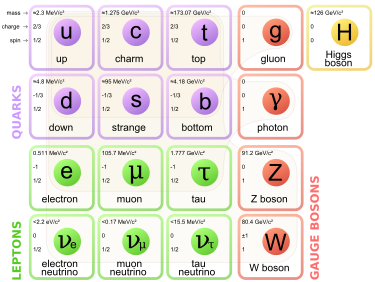
\includegraphics[width=0.9\textwidth]{Figures/StandardModel.png}
\caption{The Standard Model of particle physics.}
\end{center}
\end{figure}

hard-scattering pp collisions

\begin{equation}
\sigma_{pp \to X} = \int^1_0dx_1 \int^1_0dx_2 \sum_{a,b} f_a(x_1, \mu_F^2) f_b(x_2, \mu_F^2) \hat{\sigma}_{ab \to X}(Q^2, \mu_F^2)
\end{equation}


\subsection{Gauge theory}

Almost all of the physics within Standard Model arises directly from imposed symmetries. Interactions are produced by requiring local gauge invariance under specific symmetry groups. We define the Standard Model in group theory as the unification of two gauge symmetry groups, describing the electroweak and strong interactions. The Glashow-Weinberg-Salam electroweak model sees the electromagnetic and weak interactions combined to create the electroweak gauge symmetry group $SU(2)_L \otimes U(1)_Y$, where the gauge symmetry group for strong interactions is defined as $SU(3)_C$. Thus, we can define the gauge symmetry group of the Standard Model to be 

\begin{equation}
SU(3)_C \otimes SU(2)_L \otimes U(1)_Y.
\end{equation}

In order to explain the concept of gauge invariance we start by considering changes to the phase of the wave-functions or fields. Let us take the Lagrangian density of a free Dirac field, $\psi$, describing all free-moving spin-$\frac{1}{2}$ fermions with a mass m:  

\begin{equation} \label{eqn-DiracLagrangian}
\lumi = \bar{\psi}(i \gamma^{\mu}\partial_{\mu}-m)\psi
\end{equation}

where $\gamma^{\mu}$ are the Dirac matrices. We can show that this is invariant under phase rotations, defined by

\begin{equation}
\psi \to \psi'= e^{i \theta}\psi, \quad \bar{\psi} \to \bar{\psi}' = e^{- i \theta}\bar{\psi},
\end{equation}

as the exponential factors will cancel each out, thus we have a $U(1)$ symmetry and corresponding conserved current. This is what is known as a global phase transformation due to the time dependency of $\theta$. However, we require a local gauge invariance, and therefore a local phase transformation must be applied such that $\theta$ is different at every space-time point, which we now define as $\theta (x_{\mu})$. The local phase transformations are applied to the wave function, $\psi$, and are defined in the following way:

\begin{equation}
\psi \to \psi'= e^{i \theta(x_{\mu})}\psi, \quad \bar{\psi} \to \bar{\psi}' = e^{- i \theta(x_{\mu})}\bar{\psi},
\end{equation} 

Dropping the space-time component $\mu$ from $x_{\mu}$ for simplicity, we can see that the Dirac equation is now not invariant under the local gauge transformation as

\begin{equation}
\partial_{\mu} (e^{i\theta(x)}\psi) = i(\partial_{\mu}\theta(x))e^{i\theta(x)}\psi + e^{i\theta(x)} \partial_{\mu}\psi 
\end{equation}

which we can then express in terms of the Lagrangian as

\begin{equation}
\lumi \to \lumi - [\partial_{\mu} \theta(x)] \bar{\psi} \gamma^{\mu} \psi.
\end{equation}

In order to restore local gauge invariance, we start by hypothesising that the fermions interact with a ``gauge field" $A_{\mu}$. We can then redefine our the interacting fermion Lagrangian 

\begin{equation} \label{eqn-DiracLagrangian}
\lumi = \bar{\psi}(i \gamma^{\mu}D_{\mu}-m)\psi
\end{equation}

where we replace the ordinary derivative, $\partial_{\mu}$ covariant derivative, $D_{\mu}$, defined as

\begin{equation}
\partial_{\mu} \to D_{\mu} = \partial_{\mu} + iqA_{\mu}.
\end{equation}

where

\begin{equation}
A_{\mu} \to A_{\mu} - \partial_{\mu} \theta (x).
\end{equation}

In this way the gauge transformation of the fields cancel with that of the fermion fields, and therefore invariance is restored. The Lagrangian of Equation \ref{eqn-DiracLagrangian} is exactly what we expect for a fermion in an electromagnetic field with charge q. The second term in the Lagrangian, $-q\bar{\psi}\gamma^{\mu}A_{\mu}\psi$, describes the interaction of a fermion with a vector field with coupling strength $q=Qe$, where Q is the charge of the particle in units of e, where e is the electromagnetic coupling constant. By forcing a local $U(1)$ gauge invariance, we have essentially introduced quantum electrodynamics (QED), with the exception of the gauge field (photon) kinematic term described by the field strength tensor, $F_{\mu \nu}$, denoted  

\begin{equation}
F^{\mu \nu} = \partial^{\mu}A^{\nu} - \partial^{\nu}A^{\mu}
\end{equation}

and thus we obtain the gauge-invariant QED Lagrangian density:

\begin{equation}
\lumi_{QED} = \bar{\psi}(i \slashed{D}_{\mu} - m) \psi - \frac{1}{4}F_{\mu \nu}F^{\mu \nu}
\end{equation}

where $\slashed{D}_{\mu}$ is equal to $\gamma^{\mu}(\partial_{\mu} + iqA_{\mu})$.

We note that the gauge field $A_{\mu}$ is required to be massless in order to satisfy invariance under a local gauge transformation. This property arises as the gauge field mass term $m^2A_{\mu}A^{\mu}$ would explicitly break the gauge invariance, and thus must be removed from the Lagrangian density. Therefore we can say that QED describes Dirac fields, such as electrons and positrons, interacting with Maxwell electromagnetic force fields, photons.

By requiring local gauge invariance of the Lagrangian density by introducing additional fields in order to make it covariant with respect to an extended group of local transformations, we describe the gauge principle that is a fundamental process in particle physics. For the case of QED, we have a group of $1 \times 1$ unitary matrices multiplied by the Dirac field. The set of transformations form the Lie group $U(1)$, a group that is commutative, and thus Abelian. Gauge principle or local gauge invariant transformations can be applied to any $SU(N)$ group; Chen Ning Yang and Robert Mills first produced a theory of the $SU(2)$ gauge group \cite{PhysRev.96.191}, which was later extended to an $SU(3)$ gauge group to create QCD.  

\subsection{The Electroweak Theory} \label{subsec-ElectroweakTheory}

A theory for the unification of the electromagnetic and weak forces was first proposed by the American physicist Sheldon Glashow in 1961 \cite{Glashow:1961tr} and was later independently revised by Steven Weinberg in 1967 \cite{PhysRevLett.19.1264} and Abdus Salam \cite{Salam:1959zz} with the introduction of massive vector bosons acquiring mass by the process of spontaneous symmetry breaking. The GSW electroweak model later saw the authors receive the Nobel prize in physics in 1979. The GSW electroweak theory requires a unification of the gauge groups $SU(2)_L \otimes U(1)_Y$, where the definition of the $U(1)$ group from the previous section now refers to the unitary group of $1 \times 1$ matrices with respect to the weak hypercharge, Y, defined as 

\begin{equation}
Q = I_W + \frac{Y}{2}
\end{equation}

where Q is the electric charge, and $I_W$ is the weak isospin, also denoted $I_3$. The weak force is the only force known to violate parity, and thus distinguish between right- and left-handedness and confirmed in 1957 \cite{PhysRev.105.1413}. We can thus define left-handed doublets and right-handed singlets for fermions as so

\begin{equation}
\begin{pmatrix}
u_L \\
d_L
\end{pmatrix}
,u_R,d_R;
\quad
\begin{pmatrix}
c_L \\
s_L
\end{pmatrix}
,c_R, s_R;
\quad
\begin{pmatrix}
t_L \\
b_L
\end{pmatrix}
,t_R, b_R;
\end{equation}

for each generation of quark, and

\begin{equation}
\begin{pmatrix}
\nu_{e,L} \\
e_L
\end{pmatrix}
,e_R;
\quad
\begin{pmatrix}
\nu_{\mu,L} \\
\mu_L
\end{pmatrix}
,\mu_R;
\quad
\begin{pmatrix}
\nu_{\tau,L} \\
\tau_L
\end{pmatrix}
,\tau_R;
\end{equation}

for each generation of leptons. 

Left-handed quark and lepton doublets have weak isospin values of $I_W = 1/2$ where the upper and lower particle in each have $I^3_W = +1/2$ and $-1/2$, respectively. Right-handed particles are defined as singlets under the $SU(2)_L \otimes U(1)_L$ gauge group symmetry and thus have weak isospin of $I_W = 0$. We define left- and right-handedness by applying projection operators to the fields, such that

\begin{equation}
\psi = \frac{1}{2}(1-\gamma^5)\psi + \frac{1}{2}(1+\gamma^5)\psi = \psi_L + \psi_R,
\end{equation}

where we define the $\gamma^5$ matrix as the product of all the gamma matrices

\begin{equation}
\gamma^5 = i\gamma^0 \gamma^1 \gamma^2 \gamma^3 = 
\begin{pmatrix}
0 & 1 \\
1 & 0
\end{pmatrix}
\end{equation}

such that $\left(\gamma^5\right)^2$ is equal to the $4 \times 4$ identity matrix.

% Gell-Mann 1964 \cite{GellMann:1964nj}

Analogous to the previous case describing the $U(1)$ electromagnetic gauge group, the full covariant derivative for the electroweak theory within a $SU(2)_L \otimes U(1)_L$ gauge symmetry is given by

\begin{equation}
\partial_{\mu} \to D_{\mu} = \partial_{\mu} - ig I_W \textbf{T}^i\textbf{W}^i_{\mu} - i\frac{g'}{2}YB
\end{equation}

The $g$ and $g'$ terms represent the coupling constants for the $SU(2)_L$ and $U(1)_Y$ gauge groups, respectively; $\textbf{T}^i$ represents the three generators of the $SU(2)_L$ gauge group defined by the Pauli matrices 

\begin{equation}
\sigma_1 = 
\begin{pmatrix}
0 & 1 \\
1 & 0
\end{pmatrix}
,
\quad
\sigma_2 =
\begin{pmatrix}
0 & -i \\
i & 0
\end{pmatrix}
,
\quad 
\sigma_3 = 
\begin{pmatrix}
1 & 0 \\
0 & -1
\end{pmatrix}. 
\end{equation}

$W^i_{\mu}$ are the gauge fields that are now introduced conserve invariance in the gauge symmetry group $SU(2)_L$; and $B$ is the new gauge field for the conservation of invariance in the $U(1)_Y$ gauge symmetry group. For right-handed particle singlets, the generators $\textbf{T}^i$ are equal to 0, and thus the second term in the electroweak covariant derivative vanishes, there we can define the electroweak Lagrangian density as such

\begin{equation}
\begin{split}
\lumi_{EWK} & = \bar{\psi}_L \gamma^{\mu} \left(i \i\partial_{\mu} - g I_W \textbf{T}^i \cdot \textbf{W}_{\mu} - \frac{g'}{2} Y B_{\mu}\right)\psi_L \\
& + \bar{\psi}_R \gamma^{\mu}\left(i \i\partial_{\mu} - \frac{g'}{2} Y B_{\mu}\right)\psi_R - \frac{1}{4}\textbf{W}_{\mu \nu}\textbf{W}^{\mu \nu} - \frac{1}{4} B_{\mu \nu} B^{\mu \nu} .
\end{split}
\end{equation}

Here we define $\psi_L$ and $\psi_R$ as the double and singlet fields. Although we introduce the gauge fields $\textbf{W}^i_{\mu} and B_{\mu}$ to conserve invariance, they have no direct physical relation to gauge bosons. Instead we combine the gauge fields to form physical gauge bosons in the following linear combinations:

\begin{align}
W^{\pm}_{\mu} & = \frac{1}{\sqrt{2}}(W^1_{\mu} \pm iW^2_{\mu}), \\
Z_{\mu} & = -B_{\mu}\sin\theta_W + W^3_{\mu}\cos\theta_W, \\
A_{\mu} & = B_{\mu}\cos\theta_W + W^3_{\mu}\sin\theta_W
\end{align}   

We form the physical fields of the $W^{\pm}$ and $Z^0$ bosons, and the photon ($A_{\mu}$) by the mixing of the $W^i_{\mu}$ and $B{\mu}$ gauge fields with respect to the weak mixing angle, $\theta_W$, where we define the electric charge as:

\begin{equation}
e = g'\cos\theta_W = g \sin\theta_W.
\end{equation}

At this point we have a theory of electroweak interactions that does not incorporate electromagnetism explicitly and where a the introduction of a mass term would explicitly break invariance of the $SU(2)$ and $U(1)$ symmetries, due to the way in which right- and left-handed fermions coupling differently. Therefore, all particles must be massless in this theory. We solve this problem via the process of spontaneous symmetry breaking in the Higgs mechanism, described in Section \ref{subsec-ElectroweakSymmetryBreaking}.  

\subsection{Quantum Chromodynamics} \label{subsec-QuantumChromodynamics}

Quantum Chromodynamics (QCD) is the theory of interactions between quarks and gluons confined within hadrons by what is known as the strong force --- so called because of it's strength compared to the weak force. The theory is based upon the gauge symmetry group $SU(3)_C$, where C represents colour, the QCD analogue of electrical charge. The $SU(3)_C$ gauge group is non-Abelian under the requirement of local gauge invariance. From experimental evidence we see that quarks carry a conserved charge, which we define as ``colour" with three degrees of freedom, such that a quark can be represented as a multiplet of fields in colour space. 

\begin{equation}
r = 
\begin{pmatrix}
r \\
b \\
g
\end{pmatrix}
\end{equation}

Upon imposing invariance under $SU(3)$ gauge symmetry, we derive the Lagrangian density for QCD to be

\begin{equation}
\lumi_{QCD} & = \bar{q}\left(\gamma^{\mu}\partial_{\mu} - m \right) q + g_s \left( \bar{q}\gamma^{\mu}T_a q \right) G^a_{\mu} - \frac{1}{4}G^a_{\mu \nu}G^{\mu \nu}_a
\end{equation}

where $T_a$ represents the eight generators of the $SU(3)$ gauge group defined by the Gell-Mann lambda matrices, each $T_a$ is a $3 \times 3$ matrix in colour space which do not commute with each other and are completely anti-symmetric under the swapping of any pair of indices, and thus satisfy the lie algebra relation  

\begin{equation}
[T_a, T_b] = if_{abc}T_c.
\end{equation}

The lambda matrices represent eight massless gluon gauge fields, where $f^{abc}$ are the structure constants responsible for gluon self-interactions that arises in the field strength tensor shown in Equation \ref{eqn-QCDFieldStrengthTensor}. We note that the colour matrices and Dirac matrices do not interact as they act on different vector spaces. 

\begin{equation} \label{eqn-QCDFieldStrengthTensor}
G^a_{\mu \nu} = \partial_{\mu}G^a_{\nu} - \partial_{\nu}G^a_{\mu} + g_s f^{abc}G^b_{\mu}G^c_{\nu}
\end{equation}

As a product of self-interaction we observe two distinct properties of QCD in the form of colour confinement and asymptotic freedom. 

In a similar manner to photon exchange, the forces resulting from this type of interaction scales as $1/r^2$ at large distances, r, and thus the energy required to break up a quark-antiquark bound state is therefore finite. We have never observed quarks in isolation, but only in bound states of quark-antiquark pairs, or three-quark baryonic couplings.  

\begin{figure} \label{fig-AlphaS}
\begin{center}
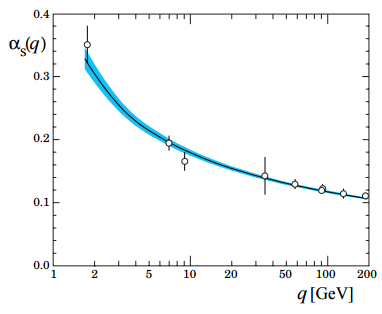
\includegraphics[width=0.5\textwidth]{Figures/AlphaS.png}
\caption{The experimentally measured values of the effective gauge coupling $\alpha_s(q)$ confirm the theoretically expected behaviour [Equation \ref{eqn-AlphaS}] at high energies (compilation of the Particle Data Group \cite{AlphaS}}
\end{center}
\end{figure}

Once we include higher-order corrections to our calculation we discover that the strength interactions mediated by vector bosons is dependent on the magnitude of q (energy-momentum transfer between partons), and it can be shown that the strong coupling constant, $\alpha_S$, can be defined as

\begin{equation} \label{eqn-AlphaS}
\alpha_s(q) = \frac{g_s(q)^2}{4\pi} = \frac{c}{log(q/\Lambda)} + ...
\end{equation}

where q is the energy-momentum transfer between partons, $\Lambda$ is the mass scale, and c is a constant. The logarithmic decay of the coupling is what we refer to as \textbf{asymptotic freedom} is observed in high-energy scattering (Figure \ref{fig-AlphaS}), such that the mass scale, $\Lambda$, has been determined to be $213^{38}_{-35}$ MeV \cite{Bethke:2000ai}\footnote{Here $\Lambda$ refers to a particular definition of the $\alpha_s$ called the $\overline{MS}$ scheme of dimensional regularisation.}. It is found that the strong coupling $\alpha_S$ decreases for interactions with higher energy, and is the reason that coloured particles are always found in colour-neutral states, as the coupling between the colour-charged states will be too strong and thus not be able to escape each other.

This prediction of QCD was first discovered in the early 1970s by H. David Polizer \cite{PhysRevLett.30.1346}, and by David J. Gross and Frank Wilczek \cite{PhysRevD.8.3633} in a completely independent study during the same year. They were subsequently awarded the Nobel prize in physics in 2004.

Another prominent aspect of QCD, which arises due to the increasing of the strong force as distance increases between quarks, is the property of \textbf{confinement}. As quarks continue to be pulled apart from one another, the energy energy rises sufficiently enough such that they form a colourless bound state, such as a quark-antiquark pair (meson), or three-quark baryonic state (baryon) as mentioned above. We call this process hadronisation, and is the reason we have never observed isolated quarks.  

%%%%%%%%%%%%%%%%%%%%%%%%%%%%%%%%%%%%%%%%%%%%%

\subsection{Electroweak Symmetry Breaking} \label{subsec-ElectroweakSymmetryBreaking}

The concept of spontaneous symmetry breaking of the electroweak symmetry first came to fruition in the 1960s and was postulated by the British physicist Peter Higgs \cite{PhysRevLett.13.508}, and independently by two groups: The first formed by the Belgian duo Francois Englert and Robert Brout \cite{PhysRevLett.13.321}, and the second by Gerald Guralnik, Carl Richard Hagen, and Tom Kibble \cite{PhysRevLett.13.585}.

we must spontaneously break the internal $SU(2)$ gauge symmetry by introducing an external field with a non-zero vacuum expectation value (vev), $\phi_c(x)$. We therefore require an $SU(2)$ doublet of complex scalar fields, $\phi$, defined as

\begin{equation}
\Phi
= 
\begin{pmatrix}
\phi^+ \\
\phi^0
\end{pmatrix}
\end{equation}

The doublet of complex scalar fields has a weak isospin, $I_W = 1/2$, and hypercharge $Y = 1$ thus leading to $+1$ for the upper members of the doublet, and 0 for the lower. Thus, in terms of real scalar fields $\phi_i$, we set

\begin{equation}
\phi^+ = \frac{\phi_1 + i \phi_2}{\sqrt{2}}, \quad \phi^0 = \frac{\phi_3 + i\phi_4}{\sqrt{2}}.
\end{equation}

The Lagrangian density for the Higgs is then created by adding the scalar contribution to the massless GSW models

\begin{equation}
\lumi_{Higgs} = (D_{\mu}\phi)^{\dagger}(D^{\mu}\phi) - V(\phi)
\end{equation}

where $D_{\mu}$ is the electroweak covariant derivative defined in Section \ref{subsec-ElectroweakTheory} such that the conjugate $\phi^{\dagger}$encompasses the antiparticles $(\phi^-\bar{\phi^0})$, and $V(\phi)$ is input as a the most general $SU(2)_L \otimes U(1)_Y$ invariant and renormalisable scalar potential defined as

\begin{equation}
V(\phi) = -\mu^2(\phi^{\dagger}\phi) + \lambda(\phi^{\dagger}\phi)^2.
\end{equation}

By defining $\lamdba < 0$ and $\mu^2 < 0$ such that $\lumi_{Higgs}$ includes a wrong-sign mass term ($-\mu^2\phi^{\dagger}\phi$). This means that the potential that we defined is now bounded below such that there will be an invariant manifold of minima that lies below $V(\phi)=0$ as we wanted. This produces what is known as the ``mexican hat" potential, as can be visualised in Figure \ref{fig-MHP}.

\begin{figure} \label{fig-MHP}
\begin{center}
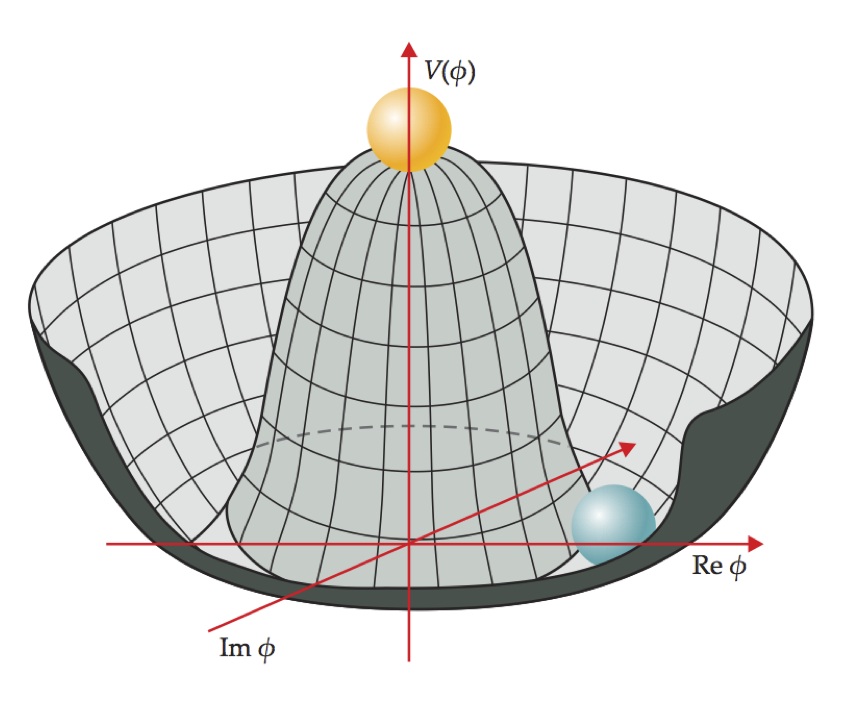
\includegraphics[width=0.7\textwidth]{Figures/MexicanHatPotential.png}
\caption{The ``Mexican Hat Potential" describing the vacuum expectation value of the Higgs in the real and imaginary planes, such that the minima lies below zero.}
\end{center}
\end{figure}

We now see that $\lumi_{Higgs}$ is invariant under a local $SU(2)_L \otimes U(1)_Y$ gauge transformation 

\begin{equation}
\phi \to \phi' = exp[-ig\frac{T^i}{2}\cdot \Delta - i\frac{g'}{2}\Lambda]\phi.
\end{equation}

We define the minima of $V(\phi)$ to be 

\begin{equation}
\frac{dV}{d(\phi^\dagger\phi)} = 0 \rightarrow \mu^2 - 2\lambda(\phi^{\dagger}\phi) = 0
\end{equation}

such that the degenerate minima are

\begin{equation}
\phi^{\dagger}\phi|_{min} = \frac{\mu^2}{2\lambda} = \frac{v^2}{2}.
\end{equation}

We then want to spontaneously break the $SU(2)_L \otimes U(1)Y$ symmetry by choosing a minimum corresponding to the lowest energy state, or vacuum. The choice of vacuum direction is in fact arbitrary, however in order for the photon to remain massless we must assign a non-zero value to a neutral field, and thus we use the conventional notation

\begin{equation} \label{eqn-HiggsDoublet}
\braket{0|\phi|0} = \frac{1}{\sqrt{2}}
\begin{pmatrix}
0 \\
v
\end{pmatrix}.
\end{equation}

$\phi$ is then expanded around the selected minimum, where we set $\phi$ to $v + H$ where H is the neutral scalar Higgs field.

\begin{equation} \label{eqn-UnitaryGauge}
\phi = \frac{1}{\sqrt{2}}
\begin{pmatrix}
0 \\
v + H
\end{pmatrix}
\end{equation}

In this way the fields with vevs set to zero, also called the ``Goldstone" fields. We can see this by applying a local gauge transformation to the field. Thus we see that a gauge transformation of Equation \ref{eqn-UnitaryGauge} is a gauge transformation of $\phi$ with four independent scalar fields. From this we arises our three massless gauge bosons, the $w^{\pm}$ and $Z^0$ which gain mass and acquire three extra longitudinal polarisation degrees of freedrom by ``absorbing" the three unphysical Goldstone bosons. We can now write the Lagrangian density as 

\begin{equation} \label{eqn-HiggsLagrangian}
\begin{split}
\lumi_{Higgs} & = \frac{1}{2}(\partial_{\mu}H)(\partial^{\mu}H) + \frac{1}{4}g^2 (H^2 + 2vH + v^2) W^+_{\mu} W^{-\mu} \\
& + \frac{1}{8} (g^2 + g'^2) (H^2 + 2vH + v^2) Z_{\mu} Z^{\mu} \\
& - \mu^2 H^2 - \frac{\lambda}{4} (H^4 + 4vH^3)
\end{split}
\end{equation}

where we used to have the relation $(g\cos\theta_W + g'\sin\theta_W)^2 = g^2 + g'^2$, but now we can directly read off the masses of the $W^{\pm}$ and the $Z^0$ by extracting the mass terms $m^2_W W^+_{\mu}W^{-\mu}$ and $\frac{1}{2}M^2_Z Z_{\mu} Z^{\mu}$ from Equation \ref{eqn-HiggsLagrangian}, where the photon still remains massless as we would expect. We can then write the masses of the bosons as 

\begin{align}
M_W & = \frac{1}{2}gv \\
M_Z & = (g^2 + g'^2)^{\frac{1}{2}}v = \frac{1}{2} \frac{gv}{\cos\theta_W}.
\end{align}
 
For the Higgs scalar, we define the mass to be 

\begin{equation}
M_H = \sqrt{2}\mu = v\sqrt{2},
\end{equation}

and as a result of the above vector boson masses we note the following relation:

\begin{equation}
\frac{M_W}{M_Z} = \cos\theta_W.
\end{equation}

This vector boson mass relation is often called the ``weak $\Delta I = 1/2$" rule, and arises by our initial choice of Higgs doublet in order to perform spontaneous symmetry breaking.

We can then use the Higgs mechanism in a similar fashion to introduce the masses for all other fermions. We do so by introducing a gauge-invariant term in $SU(2)_L \otimes U(1)_Y$ which is responsible for interactions between the Higgs and fermion fields --- the Yukawa term. We can then write a generalised Standard Model Lagrangian with the additional Yukawa terms for the first generation of fermions as such: 

\begin{equation}
\lumi_{Yukawa} = -Y^{ij}_e \bar{l}^i_L \phi e^i_R - Y^{ij}_u \bar{q}^i_L \epsilon \phi^{\dagger} u^j_R - Y^{ij}_d \bar{q}^i_L \phi d^j_R + h.c.
\end{equation}

where the Yukawa couplings, $Y^{ij}_{e,u,d}$ (e,u,d = electron, up, down), are $3\times3$ complex matrices and $\epsilon$ is the $2\times2$ antisymmetric tensor. In the Standard Model fermion masses are generated through the coupling of the Yukawa couplings to the Higgs doublet (Equation \ref{eqn-HiggsDoublet}) such that we are obtain mass terms such as:

\begin{equation}
M_e = Y_e\frac{v}{\sqrt{2}}
\end{equation}

where here we have generated, in a gauge invariant system, a mass term for the electron. By construction, a resultant feature of the Yukawa couplings is that the couplings of the Higgs boson are proportional to the masses (or squares of the masses) of particles with which it interacts. This feature is integral to the phenomenology of Higgs searches. The discovery of the Higgs boson in 2012 by both the ATLAS \cite{Aad:2012tfa} and CMS \cite{b846af59f42d440a9058d93ed5df44cf} experiments with a mass of $\sim125$ GeV, and with couplings calculated to be consistent with the Standard Model \cite{Chatrchyan:2013lba, Aad:2013wqa}. proved to be another triumph for the Standard Model. So far, we have developed a picture where we do not encounter fermions of different generations. The most successful theory of quark interactions came in the form of the CKM matrix.

\subsection{The CKM matrix}

Inspired by early work from Murray Gell-Mann and Maurice L ́evy, Italian physicist Nicola Cabibbo first introduced the Cabibbo rotation angle, $θ_c$, in 1963 \cite{PhysRevLett.10.531} in order to preserve the universality of the weak interaction. The Cabibbo angle was built on the idea that there is a relative probability for a down-type quark to decay into an up-type quark. At that time only two generations of quark were known to exist, however the charm quark was still only theorised, and so the relative probabilities only described the mixing of the up, down,
and strange quark ($V_{ud}$ and $V_{us}$ ). It was also known that the probability of an up-type quark decaying to a down-type quark is zero, which is to say that quarks of the same up or down-type cannot mix without the help of a loop.

The angle, $θ_c$, describes the rotation of the mass eigenstate vector space, formed by the mass eigenstates $\ket{d}$, $\ket{s}$, into the weak eigenstate vector space, formed by the weak eigenstates $\ket{d'}$ and $\ket{s'}$. From this we can say that the probability of an object coupling to an up-type quark through a charged weak interaction is a superposition of down-type quarks. This can be written as:

\begin{equation}
|d'> = V_{ud}\ket{d} + V_{us}\ket{s}
\end{equation}

or in terms of the Cabibbo angle 

\begin{equation}
|d'> = \cos\theta_c\ket{d} + \sin\theta_c\ket{s}
\end{equation}

Upon observing that CP violation could not be resolved within a four-quark model, Japanese physicists Makoto Kobayashi and Toshihide Maskawa sought to extend the Cabibbo rotation matrix to accommodate three generations of quark \cite{Kobayashi:1973fv}. This is written in the same manner as the Cabibbo rotation matrix, but including the top and bottom quark mixing phases, as seen in Equation \ref{eqn-ckm}, where d',s', and b' are the weak eigenstates written in terms of the mass eigenstates d,s,b. Kobayashi and Maskawa's predictions later came true when the bottom quark was discovered. Ever since the discovery of the bottom quark in 1977 at Fermilab, Chicago \cite{Innes:1977ae}, by a team led by Nobel prize-winning experimental physicist Leon Lederman, the top quark was theorised. The top quark was later discovered in 1995 with the CDF \cite{PhysRevLett.74.2626} and D0 \cite{PhysRevLett.74.2422} experiments, also at Fermilab, and thus a full third generation of quarks was in place. Kobayashi and Maskawa subsequently won the Nobel prize in physics in 2008 for their contribution to quark mixing in the Standard Model.   

\begin{equation} \label{equ-CKM}
\begin{pmatrix}
d' \\
s' \\
b' 
\end{pmatrix}
=
\begin{pmatrix}
V_{ud} & V_{us} & V_{ub} \\
V_{cd} & V_{cs} & V_{cb} \\
V_{td} & V_{ts} & V_{tb} 
\end{pmatrix}
\begin{pmatrix}
d \\
s \\
b 
\end{pmatrix}
\end{equation}

The CKM matrix describes the mixing of quark flavours where each term in the matrix represents the probability of that a quark transitioning into another quark. The values for each quark transition are given in Equation \ref{eqn-ckm}. We can see that the CKM matrix is essentially diagonal %%%%%%%%%%%%%%%%%%%%%%%%%%%%%

\begin{equation} \label{equ-ckm}
V_{CKM}
=
\begin{pmatrix}
0.97425 \pm 0.00022 & 0.2253 \pm 0.0008 & 0.00413 \pm 0.00049 \\
0.225 \pm 0.008 & 0.986 \pm 0.016 & 0.0411 \pm 0.0013 \\
0.0084 \pm 0.0006 & 0.040 \pm 0.0027 & 1.021 \pm 0.032} 
\end{pmatrix}
\end{equation}

\subsection{Where the Standard Model fails} \label{subsec-SMFailures}

\section{The Top Quark} \label{sec-TheTopQuark}

The top quark is the heaviest of all the fundamental particles and was first postulated, along with the bottom quark, in 1973 by Makoto Kobayashi and Toshihide Maskawa \cite{Kobayashi:1973fv} to explain the observations of CP violation in the kaon sector. It was with the discovery of the $\tau$ lepton \cite{PhysRevLett.35.1489} in 1975, and then the discovery of the bottom quark in 1977 \cite{Innes:1977ae} and the quark-lepton generation symmetry which lead to the postulation of the top quark. Event with the discovery of the W and Z bosons in 1985 with the UA1 \cite{ARNISON1983103} and UA2 \cite{Banner1983476} experiments at the Super Proton Synchrotron (SPS), CERN, the top quark was still nowhere to be seen, and at this point in time there was still no experimental apparatus capable of reaching the required energies needed to discover the top. It was in 1995 when the CDF \cite{PhysRevLett.74.2626} and D0 \cite{PhysRevLett.74.2422} experiments at the Tevatron (Fermilab, Illinois) first observed the top quark, which subsequently prompted Kobayashi and Maskawa to win the Nobel prize for their predictions in 2008.

The most up-to-date measurement of the top mass has been calculated by combining results from the LHC and the Tevatron to be $173.34 \pm 0.27(stat.) \pm 0.71(syst.)$ GeV/c$^2$ \cite{ATLAS:2014wva}. sAs a direct result of the top quarks extremely large mass, it has a very short decay time which is shorter than the time required for quarks to hadronise and form composite particles with other quarks. The decay time of the top is approximately $5 \times 10^{-25}$ s \cite{Quadt:2007jk}, whereas the hadronisation time for quarks is given as $\tau_{had.} \approx 1/\Lamdba_{QCD} \aprox 10^{-23}$ s \cite{0954-3899-37-7A-075021}. Thus, we never observe $t\bar{t}$ bound states and the information relating to spin is inherited by the decay products of the top. Therefore the top quark provides unique opportunities to study precision tests of the Standard Model.

\begin{equation}
\sigma_{pp \to t\bar{t}+X} = \sum_{i,j} \int^1_0 dx_1 \int^1_0 dx_2 f_1(x_i, \mu_F)f_2(x_j, \mu_F)\hat{\sigma}_{i,j \to t\bar{t}}(\hat{s})
\end{equation}

\subsection{Top quark anomalous couplings}

The measurement of the couplings between the known fermions and bosons is a standard tool in the search for physics beyond the Standard Model. At the LHC top quarks are produced in copious amounts, allowing us to probe top couplings to a great precision. The large mass of the top quark is directly related to the effects of new physics on its couplings such that deviations from Standard Model predictions may be detectable, therefore the LHC provides the perfect environment in which to study such effects.

The top quark provides a direct test of the quark-photon vertex which is unique among the quarks, thus there is great interest as to the determination of the coupling of the top quark and photon, and probing the $t\bar{t}\gamma$ channel at the LHC with an energy of 8 TeV provides directly explore the top quarks role in the mechanism of electroweak symmetry breaking. Any deviation from that of SM prediction would imply an anomalous structure of the quark-photon vertex, and would thus reveal any physics beyond that of the Standard Model, such as exotic quarks, SUSY, technicolour. 

In order to successfully create a model of interactions between fermions and bosons, we require a good enough parametrisation of the interactions in the form a Lagrangian. We can write a general parametrisation for the on-shell interaction of two fermions ($f_i$, $f_j$) and a boson ($V = W,Z,\gamma,g$) as

\begin{equation}
\begin{split}
\lumi^{OS}_{Vf_if_j} = & \bar{f}_j\gamma^{\mu} (\mathcal{A}_L P_L + \mathcal{A}_R P_R)f_i V_{\mu} \\
& + \bar{f}_j i \sigma^{\mu \nu} q_{\nu}(\mathcal{B}_L P_L + \mathcal{B}_R P_R) f_i V_{\mu} + \text{h.c.}
\end{split}
\end{equation}

where $q = p_i - p_j$ is the momentum of the outgoing boson and $\mathcal{A}_{L,R}$, $\mathcal{B}_{L,R}$ are form factors, which in general may depend on $q^2$, however for the flavour-conserving photon and gluon vertices we have $\mathcal{A}_L = \mathcal{A}_R$ and for flavour-changing $\mathcal{A}_{L,R} = 0$ due to gauge symmetry. 

A set of dimension-six gauge-invariant operators, $O_x$, known as effective operators, can be found to parametrise quark couplings up to a scale $\Lambda$ \cite{anom-coups}. They appear linearly in an interaction Lagrangian, which is written in the form of a Taylor expansion, with complex effective coefficients $C_x$:

\begin{equation} \label{eqn-EffectiveOperators}
\lumi^{eff.} = \Sum \frac{C_x}{\Lambda_x}O_x + ... ,
\end{equation}

Among the operators defined in the effective Lagrangian \cite{Buchmuller:1985jz} fourteen contribute to the electroweak anomalous couplings. These are as so:

\begin{align}
& O^{(3, i, j}_{\phi q} = i(\phi^{\dagger}\tau^I D_{\mu} \phi)(\bar{q}_{Li}\gamma^{\mu}\tau^I q_{Lj}), \quad & O_{ij}_{Du} = (\bar{q}_{Li} D_{\mu} u_{Rj}) D^{\mu} \tilde{\phi}, \\
& O^{(1, i, j)}_{\phi q} = i(\phi^{\dagger} D_{\mu} \phi)(\bar{q}_{Li}\gamma^{\mu} q_{Lj}), \quad & O_{ij}_{\bar{D}u} = (D_{\mu} \bar{q}_{Li} u_{Rj}) D^{\mu} \tilde{\phi}, \\
& O^{ij}_{\phi \phi} = i(\phi^{\dagger} D_{\mu} \phi)(\bar{u}_{Ri}\gamma^{\mu} d_{Rj}), \quad & O_{ij}_{Dd} = (\bar{q}_{Li} D_{\mu} d_{Rj}) D^{\mu} \phi, \\
& O^{ij}_{\phi u} = i(\phi^{\dagger} D_{\mu} \phi)(\bar{u}_{Ri}\gamma^{\mu} d_{Rj}), \quad & O_{ij}_{\bar{D}d} = (D_{\mu} \bar{q}_{Li} d_{Rj}) D^{\mu} \phi, \\
& O^{ij}_{uW} = (\bar{q}_{Li} \sigma^{\mu \nu} \tau^I u_{Rj})\tilde{\phi} W^I_{\mu \nu}, \quad & O_{ij}_{qW} = \bar{q}_{Li} \gamma^{\mu} \tau^I D^{\nu} q_Lj W^I_{\mu \nu}\\
& O^{ij}_{dW} = (\bar{q}_{Li} \sigma^{\mu \nu} \tau^I d_{Rj})\phi W^I_{\mu \nu}, \quad & O_{ij}_{qB} = \bar{q}_{Li} \gamma^{\mu} D^{\nu} q_Lj B_{\mu \nu}\\
& O^{ij}_{uB\phi} = (\bar{q}_{Li} \sigma^{\mu \nu} u_{Rj})\tilde{\phi} B_{\mu \nu}, \quad & O_{ij}_{uB} = \bar{u}_{Ri} \gamma^{\mu} D^{\nu} u_Rj B_{\mu \nu}
\end{align}

for different flavours represented by the indices $i,j = 1,2,3$. $\bar{q}_{Li}$, $u_{Ri}$, and $d_{Ri}$ represent the quark fields as shown in Section \ref{subsec-ElectroweakTheory}. The operators where we have $i = j = 3$ contribute to the electroweak coupling processes $Wtb$, $Zt\bar{t}$, and $\gammat\bar{t}$. 

\subsection{The top-photon vertex}

\begin{figure} \label{fig-TopPhotonVertex}
\begin{center}
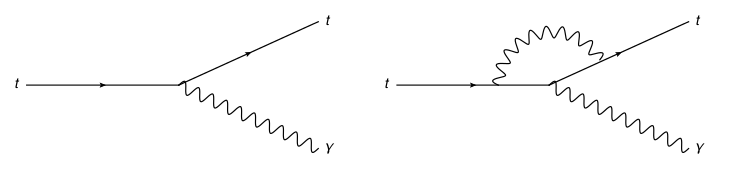
\includegraphics[width=\textwidth]{Figures/TopPhotonVertex.png}
\caption{Top-photon vertex. Left: Leading Order (LO). Right: One-Loop correction (NLO).}
\end{center}
\end{figure}

The general expression for the interaction Lagrangian for the top-photon ($\gamma t \bar{t}$) vertex (shown in Figure \ref{fig-TopPhotonVertex}) can be parametrised in terms of the dimension-six operators and written, not including the redundant operators, in the form \cite{anom-coups}:

\begin{equation} \label{eqn-interactionlagrangian}
\lumi_{\gamma t\bar{t}} = -eQ_t\bar{t}\gamma^{\mu}tA_{\mu} - e\bar{t}\frac{i\sigma^{\mu\nu}q_{\nu}}{m_t}(d^{\gamma}_V+id^{\gamma}_A\gamma^5)tA_{\mu}
\end{equation}

The first term in Equation \ref{eqn-interactionlagrangian} is a purely SM contribution, and is linear with respect to electrical charge of the top, $Q_t$, such that the bare $t\bar{t}+\gamma$ cross-section is proportional to the square of the top-quark charge. The second term is described by the vector and axial form factors, $d^{\gamma}_V$ and $d^{\gamma}_A$, which arise from the contributions of first-order loop corrections, representing the magnetic and electric dipole moment of the top quark (where the latter is CP-violating), respectively. The couplings, $d^{\gamma}_V$ and $d^{\gamma}_A$, are real and comprise the operators $O^{33}_{uB\phi}$ and $O^{33}_{uW}$ from the eight effective operators described previously mentioned. They parametrise deviations from SM expectations of the form factors, $d^{\gamma}_V$ and $d^{\gamma}_A$, as such:

\begin{align}\label{eqn-smparameterisations}
\delta d^{\gamma}_V = \frac{\sqrt{2}}{e}\text{Re}[c_WC^{33}_{uB\phi} + s_WC^{33}_{uW}]\frac{vm_t}{\Lamdba^2} \\
\delta d^{\gamma}_A = \frac{\sqrt{2}}{e}\text{Im}[c_WC^{33}_{uB\phi} + s_WC^{33}_{uW}]\frac{vm_t}{\Lamdba^2}
\end{align}

where $\delta d^{\gamma}_V$ and $\delta d^{\gamma}_A$ only receive non-zero contributions from phenomena beyond the SM. We are able to obtain a measurement of these constants by analysing the magnetic and electric dipole moments of the top quark. We note that the $\gamma^{\mu}$ term does not receive corrections from the dimension-six operators. If we had included the redundant effective operators ($O_{Wq}$, $O_{Bq}$, $O_{Bu}$) then the first two would incorporate additional corrections of $\sim q^2 \bar{t}_L \gamma^{\mu} t_R A_{\mu}$ and the last $q^2 \bar{t}_R \gamma^{\mu} t_R A_{\mu}$, no-vanishing only when the photon is off-shell.

The magnetic dipole moment of the top quark is studied by measurements of spin correlation, whereas the electric dipole moment can be investigated through the $t\gamma$ vertex. Deviations from SM contributions are expected to manifest in the photon energy spectrum and angular photon distributions.

Measuring $t\bar{t}+\gamma$ provides a direct test of the electromagnet coupling of the top quark in a way that is complementary to analyses that include an ``exotic" top quark with a charge of -4/3e \cite{top-charge}. One issue when investigating the $t\bar{t}+\gamma$ process is the large irreducible background of photons that are radiated by charged particles other than the top quark. It has also been proved that the interference of photon production from initial state radiation (ISR) and final state radiation (FSR) can not be deemed negligible \cite{topchargemeasurement}. This is also discussed with respect to Monte Carlo signal generation in Section \ref{sec-mcsim}. Thus only inclusive observables of $t\bar{t}+\gamma$ can be probed, as we are unable to trace the photon back to its parent particle. We will also treat on- and off-shell radiation collectively. We will discuss prompt photon backgrounds in Section \ref{chap-EventSelection}. 

\subsection{Previous measurements}

Presently, the determination of the operators $C^{33}_{uB\phi}$ and $C^{33}_{uW}$ is not possible due to the statistical significance of recorded events at the LHC being low. This will become more accessible at higher centre-of-mass energy and luminosity. Until then, benchmark studies have been undertaken \cite{pidsemilept}.

The CDF experiment at the Tevatron, along with the CMS and ATLAS experiments at the LHC, have measured the inclusive $t\bar{t}+\gamma$ production cross-section at $\sigma^{CDF}_{t\bar{t}+\gamma} = 0.18 \pm 0.08$ pb \cite{CDFttgamma}, $\sigma^{CMS}_{t\bar{t}+\gamma} = 2.4 \pm 0.2 (\text{stat}) \pm 0.6 (\text{syst.})$ \cite{CMS-PAS-TOP-13-011}, and $\sigma^{ATLAS}_{t\bar{t}+\gamma} = 2.0 \pm 0.5 (\text{stat}) \pm 0.7 (\text{syst.}) \pm 0/08 (\text{lumi})$ pb at 7 TeV \cite{ATLASttgamma}, respectively. The SM expectations for these values are given as $\sigma^{Tevatron}_{t\bar{t}+\gamma} = 0.17 \pm 0.003$ pb and $\sigma^{LHC}_{t\bar{t}+\gamma} = 2.1 \pm 0.4$ pb, respectively, and thus the measurements observed are in accordance to those theorised. 

In relation to the electrical charge of the top quark, the CMS and ATLAS experiments have also performed analyses, hypothesis tests, where the final state charges of the top quark are combined, and both yield similar results. The experiments concluded that an electrical charge of $Q_t = -4/3e$ could be excluded  with a high significance \cite{topchargeconstraints, ATLAStopcharge}.

Other top quark couplings have been measured at the Tevatron and the LHC, also. The structure of the $Wtb$ vertex has been investigated in helicity measurements of top quark correlated W bosons at the Tevatron and LHC, putting limits on anomalous couplings \cite{CDFD0combination, Whelicitytoppair, Wpolarisation}. The strength of $tW$ couplings can be tested through single top quark production and has been found to be consistent with SM expectations \cite{tsinglet, singlet}. Also, the inclusive $t\bar{t}W$ and $t\bar{t}Z$ production cross-sections have been measured by CMS to be $\sigma_{t\bar{t}W} = 170^{+90}_{-80}(\text{stat}.) \pm 70(\text{syst}.)$ fb and $\sigma_{t\bar{t}Z} = 200^{+80}_{-70}(\text{stat}.) ^{+40}_{-30}(\text{syst}.)$ fb, respectively, with the combined $t\bar{t}V$ cross-section as $\sigma_{t\bar{t}V} = 380^{+100}_{-90}(\text{stat}.)^{+80}_{-70}(syst.) $ fb, and exclusion limits on anomalous couplings are set \cite{Khachatryan:1712680}. Another focus in the area is flavour changing neutral currents (FCNC) in top decays, $t \to qZ$ and $t \to q\gamma$ are also currently being studied. Limits are set for these processes \cite{tqZ, FCNC}, which confirm SM FCNC suppression. 

It is important to note that a measurements of $t\bar{t}+\gamma$ are extremely challenging at the LHC with the current centre-of-mass energy and luminosity. This is due to the limited four-momentum resolution of partons, pile-up, and large background from QCD multi-jet events. It has been estimated that a 10\% resolution of the top quark's charge will be available at $\sqrt{s} = 14$ TeV with 10 fb$^{-1}$ \cite{topchargemeasurement}. As teh energy is increased at the LHC the gluon fusion process becomes more dominant and thus fewer photons can be emitted in the form of initial state radiation. A high energy $e^+e^-$ collider would be preferable for this study as it would be a much cleaner working environment, such that we could obtain a 5--10\% precision on axial form factor $d&{\gamma}_A$ can be achieved with 10 fb$^{-1}$ at $\sqrt{s} = 500$ GeV \cite{linearcollider}.


\begin{table} \label{tab-}
\begin{center}
\begin{tabular}{lccc}
\hline
\hline
\textbf{$\sqrt{s}$} & \textbf{$\sigma_{tot.}$} & \textbf{scales [pb]} & \textbf{pdf [pb]} \\
\hline
Tevatron 1.9 TeV & 7.164 & & \\
LHC TeV & 172.0 & $^4.4_5.8$ &  \\ 
LHC 8 TeV & 245.8 & & \\
LHC 14 TeV & 953.6 & & \\
\hline
\hline
\end{tabular}
\caption{\cite{Czakon:2013goa}}
\end{center}
\end{table}

\begin{figure} \label{fig-ttbarProductionLHC}
\begin{center}
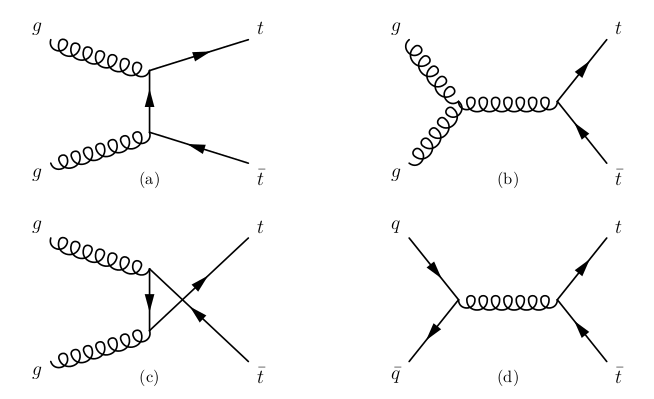
\includegraphics[width=\textwidth]{Figures/ttbarProductionLHC.png}
\caption{Lowest level diagrams for $t\bar{t}$ production at the LHC. Gluon scattering processes, {(a)}, {(b)}, and {(c)}, are the dominant processes at LHC energies, while quark scattering, process {(d)}, is the dominant one at TeVatron energies. \cite{SergeyThesis}}
\end{center}
\end{figure}

\begin{figure} \label{fig-singletopProductionLHC}
\begin{center}
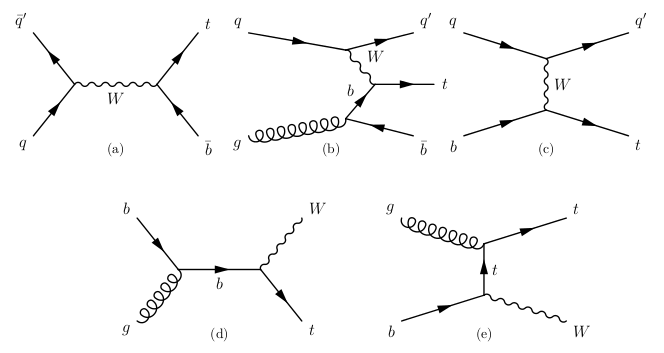
\includegraphics[width=\textwidth]{Figures/singletopProductionLHC.png}
\caption{Leading-order level diagrams for single top production at the LHC. {(a)} s-channel, {(b)} and {(c)} represent the t-channel, {(d)} and {(e)} both represent the two tW channels. \cite{SergeyThesis}}
\end{center}
\end{figure}

\begin{figure}
\begin{center}
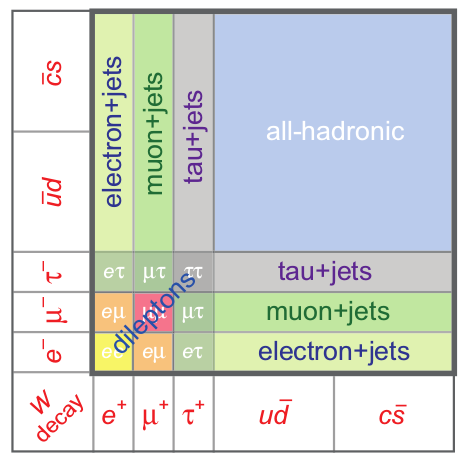
\includegraphics[width=0.5\textwidth]{Figures/ttbarDecayFractions.png}
\caption{Branching fractions of the W decays within top quark pairs. \cite{ttbarDecayFractions}}
\end{center}
\end{figure}

\begin{figure} \label{fig-ttgammaFeynmanDiagram}
\begin{center}
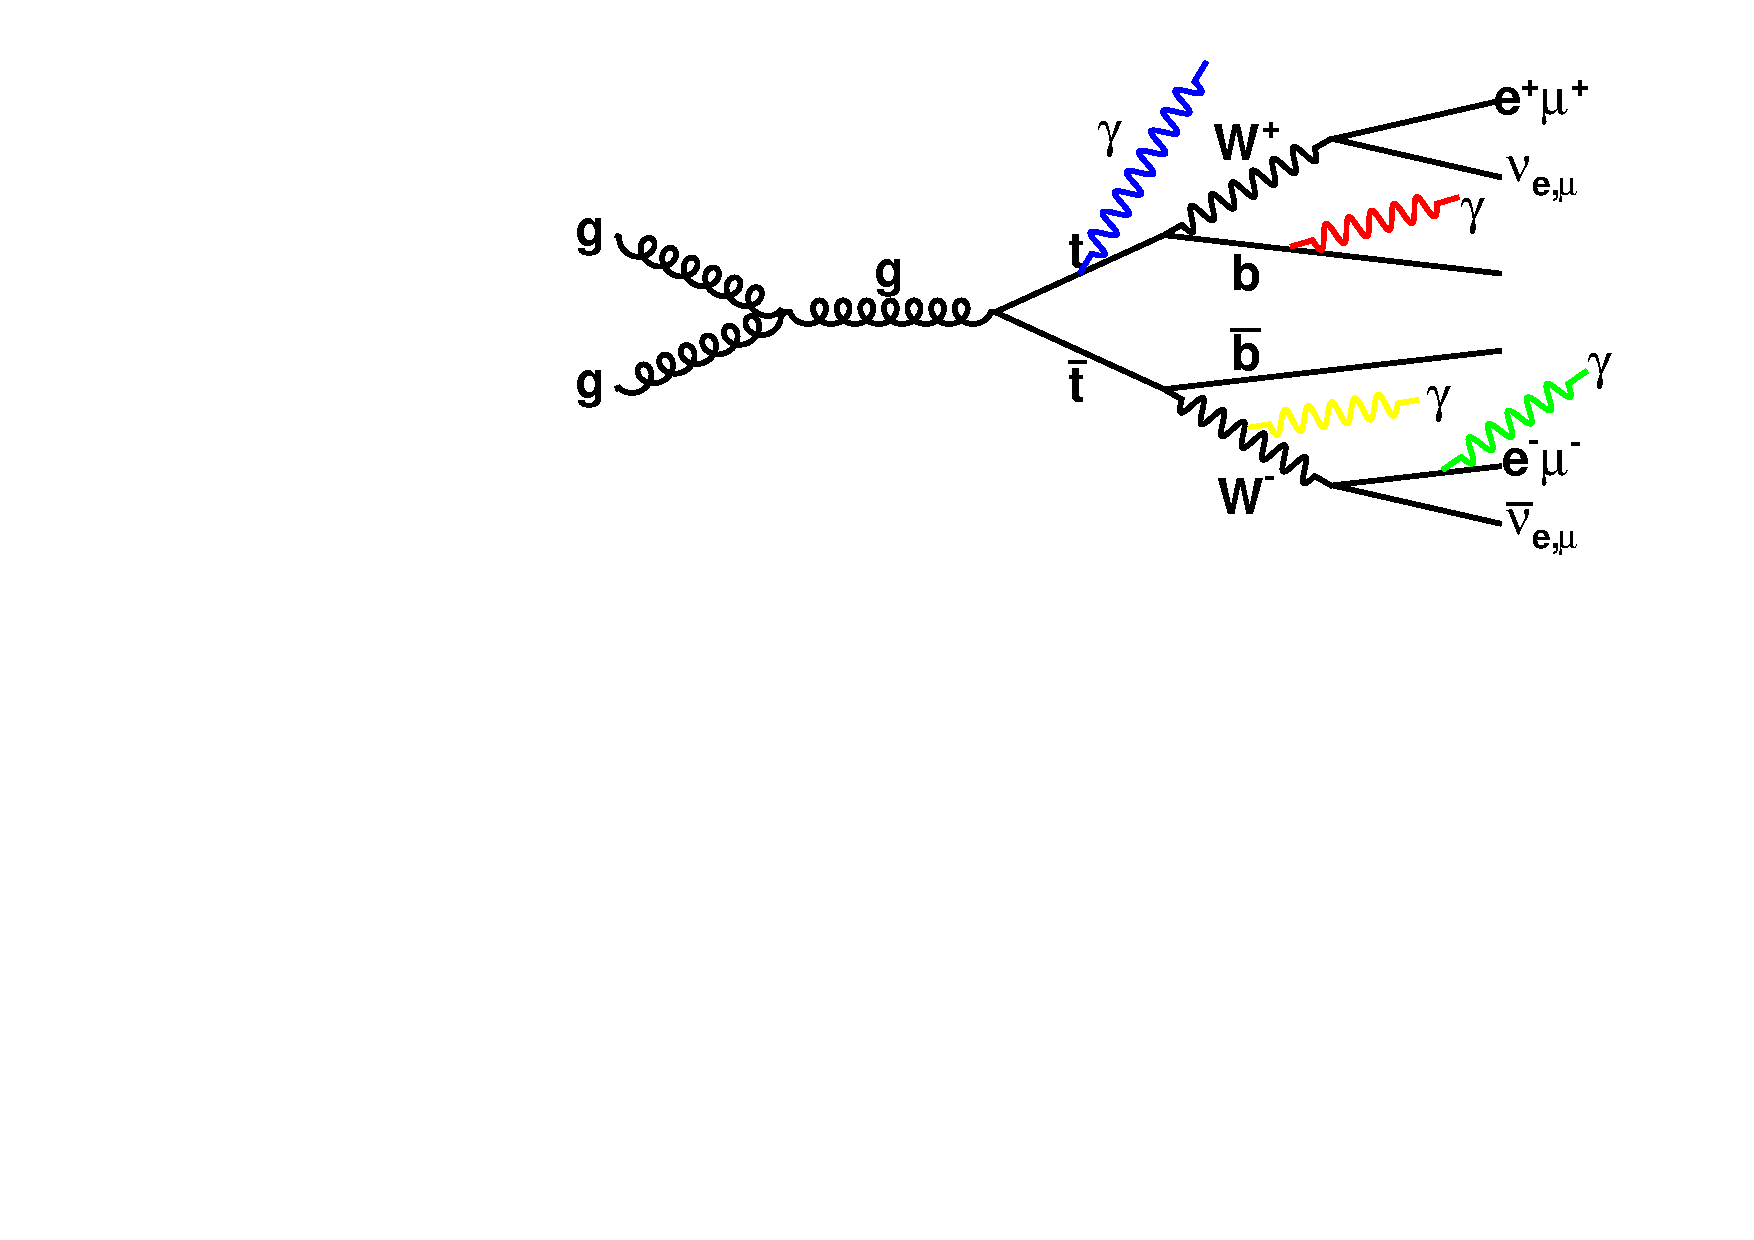
\includegraphics[width=0.9\textwidth]{Figures/ttgammaFeynmanDiagram.pdf}
\caption{}
\end{center}
\end{figure}

\chapter{The LHC and the CMS Detector} \label{chap-detector}

\section{The Large Hadron Collider} \label{sec-TheLargeHadronCollider}

The Large HAdron Collider (LHC) is currently the largest, and highest energy, particle accelerator ever created. Located, on average, one hundred metres under the Franco-Swiss border at Geneva, the LHC is installed in the 26.7 km tunnel that once contained the Large Electron-Positron Collider (LEP) which ran from 1989 until the end of 2000. The project was approved by the CERN council in December of 1994. Originally, the accelerator was designed as a two-stage project: constructed to run at a centre-of-mass energy of $\sqrt{s}=7$ TeV, and later an upgrade to $\sqrt{s}=14$ TeV. This was due to budget constraints which did not include contributions from non member states. 

After many setbacks, the first run began in 2010 and continued until the end of 2011 when the beam energy was then increased to $\sqrt{s}=8$ TeV for the whole of 2012 before shifting to Long Shutdown 1 (LS1) from 2013 to 2015. During LS1 the CERN accelerator complex, shown in Figure \ref{fig-CERNAcceleratorComplex}, was completely upgraded in order to run at a new unprecedented centre-of-mass energy of $\sqrt{s}=13$ TeV before ramping up to the original design energy of $\sqrt{s}=14$ TeV. 

\begin{figure}\label{fig-CERNAcceleratorComplex}
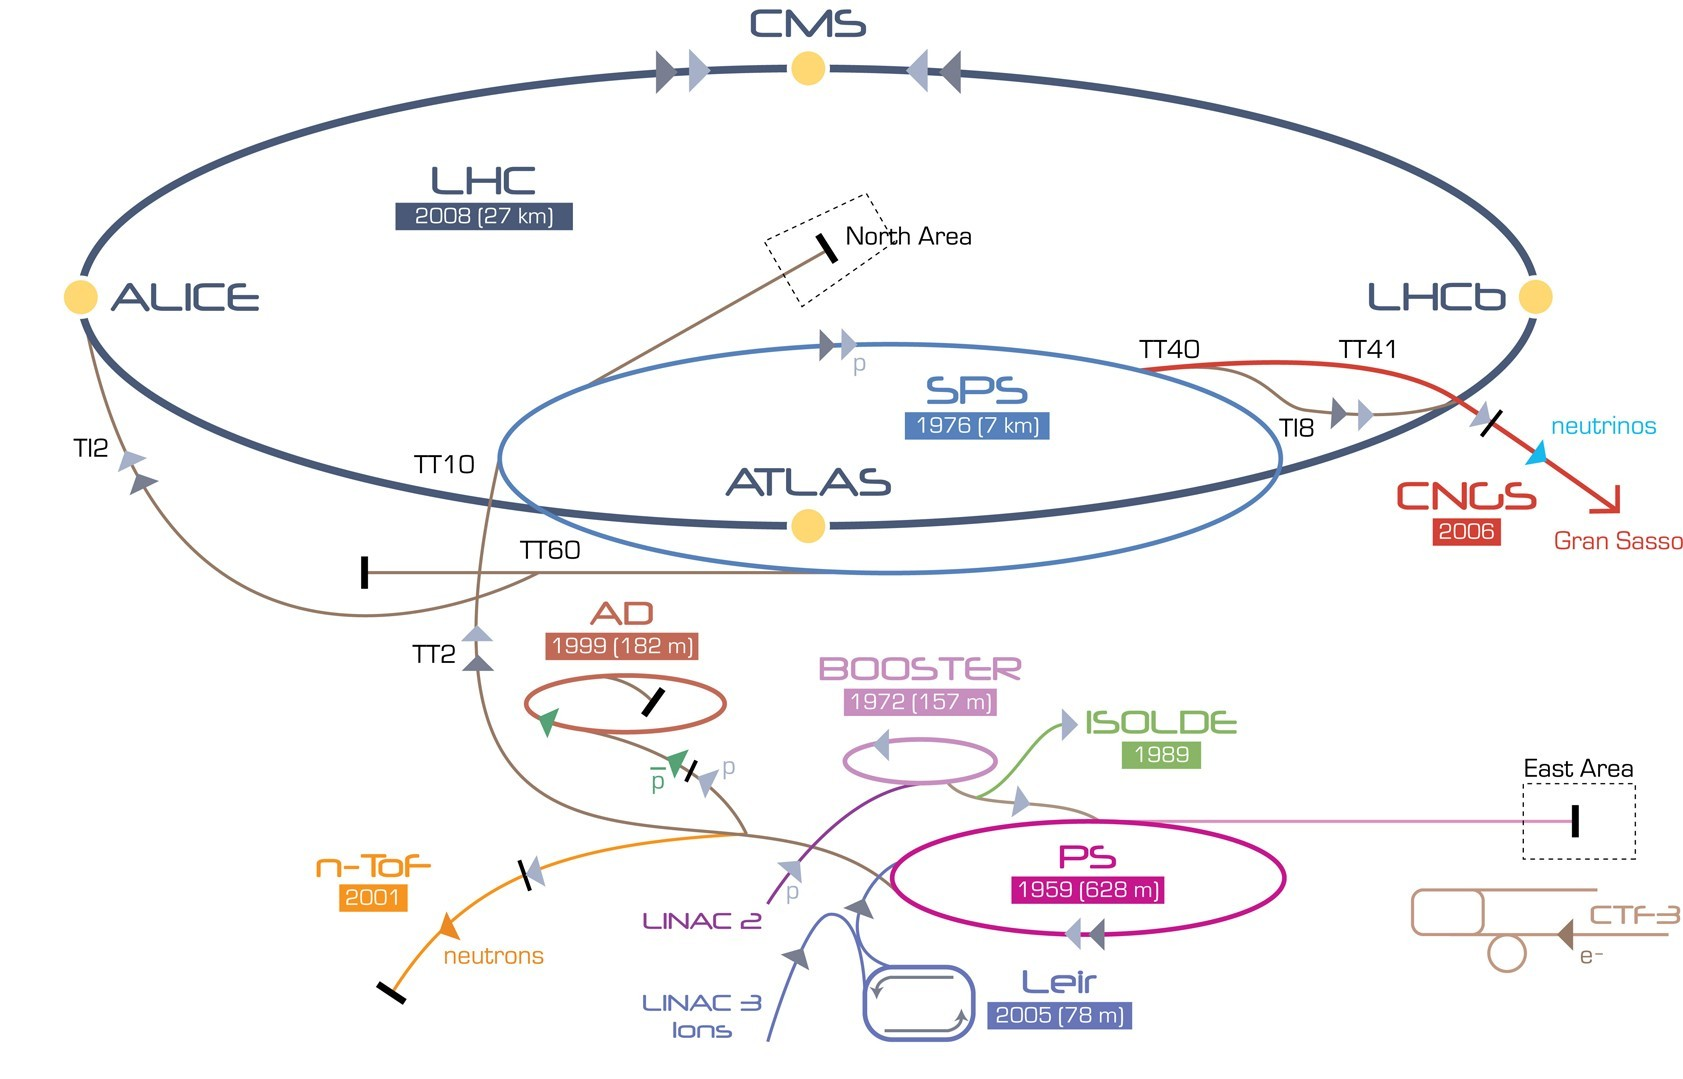
\includegraphics[width=\textwidth]{Figures/CERNAcceleratorComplex.jpg}
\caption{A full schematic of the full CERN accelerator complex.}
\end{figure}

\subsection{Pre-LHC accelerator complex}

The proton acceleration process begins by injecting Hydrogen ($H_2$) gas into a Duoplasmatron surrounded by an electric field, whereby the electrons become ionised through interactions with the free electrons from the cathode forming a plasma. This strips the electrons from the Hydroden leaving just the protons. The remaining protons are then linearly accelerated by the LINAC 2 accelerator, which uses radio frequency (RF) cavities to accelerate bunches of protons. By the end of this step the protons have reached an energy of up to 50 MeV and gained 5\% in mass. The next stage in the sequence sees the protons enter the Proton Synchroton Booster (PSB) which is composed of superimposed sychrotron rings which accelerate the received protons up to 1.4 GeV in 1.2 seconds before injection into the Proton Sychrotron (PS). The advantage of the Booster is that it allows the PS to accept over 100 times more protons by squeezing the proton bunches such that they have a much smaller cross-section. 

The PS is an essential component in the accelerator complex at CERN, where it accelerates either protons received from the PSB, or heavy ions from the Low Energy Ion Ring (LEIR). The apparatus first ran on the 24th of November 1959, and was, at that time, the worlds highest energy particle accelerator. Having a circumference of 628 metres, the PS comprises 277 conventional (room temperature) electromagnets, as well as 100 dipole magnets that serve to bend the beam around the ring. The PS accelerates protons, as well as other particles, up to 25 GeV in 3.2 s. The final stage of acceleration, before injection into the LHC, lies in the Super Proton Sychrotron (SPS). The SPS is the second largest of the CERN accelerators with a circumference of 7 kilometers, and provides beams for various experiments other than LHC: such as the NA61/SHINE and NA62 experiments, the COMPASS experiment, and the CNGS neutrino experiment. Protons are accelerated to 450 GeV  in 20 s within the SPS before injection into the LHC. Before the creation of LEP or the LHC the SPS was the primary collider at CERN, and in 1983 the collaboration won the Nobel prize for the discovery of the W and Z bosons in proton-antiproton collisions. The SPS comprises 1317 conventional electromagnets and 744 dipoles.

\subsection{Design of the LHC}

Two beams of protons are injected into the LHC and accelerated using RF cavities, one clockwise and the other counter-clockwise, taking roughly 20 minutes for each beam to reach the design energy of 7 TeV per beam. The two beams come into collision at four points around the $\sim27$ km ring where the collisions are recorded by the four detectors placed on the beam line. There are two all-purpose discovery detectors, namely CMS and ATLAS, studies of mesons by LHCb, and the study of heavy ions by the ALICE experiment. Because the tunnel in which the LHC is placed was designed for LEP it has an internal diameter of only 3.7 m, which is not large enough to install two separate beam pipes, and thus a design for a twin-bore magnet \cite{LHCStorageAccelerators}was created which would save space and cut costs substantially. Each beam is designed to hold 2808 bunches of protons with a bunch spacing of 50 ns. The protons are guided around the ring in a vacuum by superconducting electromagnets which are cooled to 1.9 K (-271.3$^\circ$) by using liquid helium. It consists of 1232 dipole magnets that are each 15 metres in length, and 392 quadrupole magnets that are 5-7 metres in length each which focus the beams. Before collisions can begin, a final shaping and cleaning of the beam takes place. Parameters for the LHC can be seen in Table \ref{tab-LHCparameters}.

\begin{table} \label{tab-LHCparameters}
\begin{center}
\begin{tabular}{|l|c|c|}
\hline
	\multicolumn{3}{|c|}{\textbf{LHC Parameters}} \\
\hline
	\textbf{Parameter} & \textbf{2012 Run} & \textbf{Design Value} \\
\hline	
	Beam Energy (TeV) & 4 & 7 \\
	Maximum number of bunches  & 1380 & 2808 \\
	Number of particles per bunch & $1.7\times 10^{11}$ & $1.15\times 10^{11}$ \\
	Bunch spacing (ns) & 50 & 25 \\
	Revolution frequency (kHz) & 11.245 & 11.245 \\
	Transverse beam size ($\mu$m) & 18.8 & 16.6 \\
	Peak luminosity (cm$^{-2}$s$^{-1}$) & $7.7\times 10^{33}$ & $10^{34}$ \\
	Stored beam energy (MJ) & 140 & 362 \\
	Normalised emittance at start of fill (mm mrad) & 2.5 & 3.75 \\
	$\beta^*$ in IP 1 and 5 (m) & 0.6 & 0.55 \\
\hline
\end{tabular}
\end{center}
\caption{LHC design parameters \cite{LHCDesignReport}.}
\end{table}


\subsection{Physics goals}

 There are many physics goals aimed to be achieved during the running of the LHC, but there are certain aims that are of a higher priority than others. One of the main focuses was the discovery of the Higgs boson and electroweak symmetry breaking, which was announced on the fourth of July 2012. This discovery was a triumph for the physics community in that it shed light on a fundamental building block of the universe which was theorised to exist some sixty years before its discovery. The theoretical physicist Peter Higgs subsequently won the Nobel prize for his work predicting the existence of a massive gauge boson in 1964. The Higgs a since been measured in various decay channels by both they ATLAS and CMS experiments with on-going studies aiming to measure properties of the boson, such as a the spin. Other physics goals include the search for supersymmetry, CP violation measurements, and studies of quark-gluon plasma using the ALICE experiment.  

\subsection{Luminosity at the LHC}

Due to the nature of individual detectors, not all require the same levels of delivered luminosity. For example, with CMS being an all-purpose discovery machine, the detector needs as much luminosity as possible, however an experiment like LHCb that measure mesons that are produced frequently and in a certain portion of the solid angle that the others use, less luminosity is required. The peak design luminosities for Run I and Run II are listed in Table \ref{tab-LHCparameters}. The instantaneous luminosity of a collider is calculated as

\begin{equation}
\mathcal{L}=f\frac{N_1N_2}{4\pi\sigma_x\sigma_y}
\end{equation}

where f is the collision frequency given by $f=u\times N_b$, the repetition frequency multiplied by the number of bunches in the beam, $N_{1,2}$ are the number of protons per bunch per beam, and $\sigma_{x,y}$ are the horizontal and vertical beam sizes at the interaction point (IP), respectively, and are defined as the product of the beams beta function and the proton beam emittance as shown in Equation \ref{eqn-beamsize}.

\begin{equation} \label{eqn-beamsize}
\sigma_{x,y}=\epsilon_{x,y}\beta_{x,y}
\end{equation}

The emittance of a beam describes the volume of the 6-dimensional phase space occupied by the proton bunch.

\subsection{Performance throughout run I}

Throughout Run I (2010 - 2013) the LHC operated with protons at beam energies of 3.5 and 4 TeV, where the beams consisted of single bunches and trains with different bunch spacing of 150 ns (2010), 75 ns (2011), and 50 ns (2011 and 2012). The performance of the LHC was much greater than initially expected at 50 ns, and culminated in the discovery of a $125 GeV/c^2$ Higgs boson in both the ATLAS \cite{ATLASHiggs} and CMS \cite{CMSHiggs} experiments. The use of 25 ns bunch spacing was only implemented in regards to electron-cloud scrubbing runs at the injection stage, and also for tests of future collisions with an upgraded LHC energy. One of the main focuses was to reduce the $\beta^*$ - the measure of how precisely the beam is focused at the interaction point. For ATLAS and CMS $\beta^*$ was lowered in steps from 3.5 mm in 2010 to 0.6 mm in 2012 by using tighter collimator settings. Other runs with mixed particle beams were also performed: such as proton-Pb, Pb-Pb, intermediate proton energy (1.38 TeV), and high beta.

For the 2012 run the default filling scheme introduced 1374 proton bunches per beam with 50 ns bunch spacing, giving ATLAS and CMS 1368 colliding bunches, 1262 in LHCb, and no colliding bunches in ALICE. The bunch intensity per beam peaked at $1.7 \times 10^{11}$ protons per bunch, which was then translated into a bunch intensity of $1.6 \times 10^{11}$ protons per bunch upon stabilisation of the beams. The transverse emittance remained constant throughout the year, despite moving to a different optical configuration with a lower transition energy. At the end of the runs the LHC had delivered an integrated luminosity of 23.3 fb$^{-1}$ to ATLAS and CMS, and over 2.1 fb$^{-1}$ to LHCb. The integrated and peak luminosity can be seen in Figure \ref{fig-LHClumi}, and the integrated luminosity recorded by CMS between 2011 ans 2013, and also compared to the total integrated luminosity delivered by the LHC, can be seen in Figure \ref{fig-CMSlumi}.

\newpage

\begin{figure} \label{fig-LHClumi}
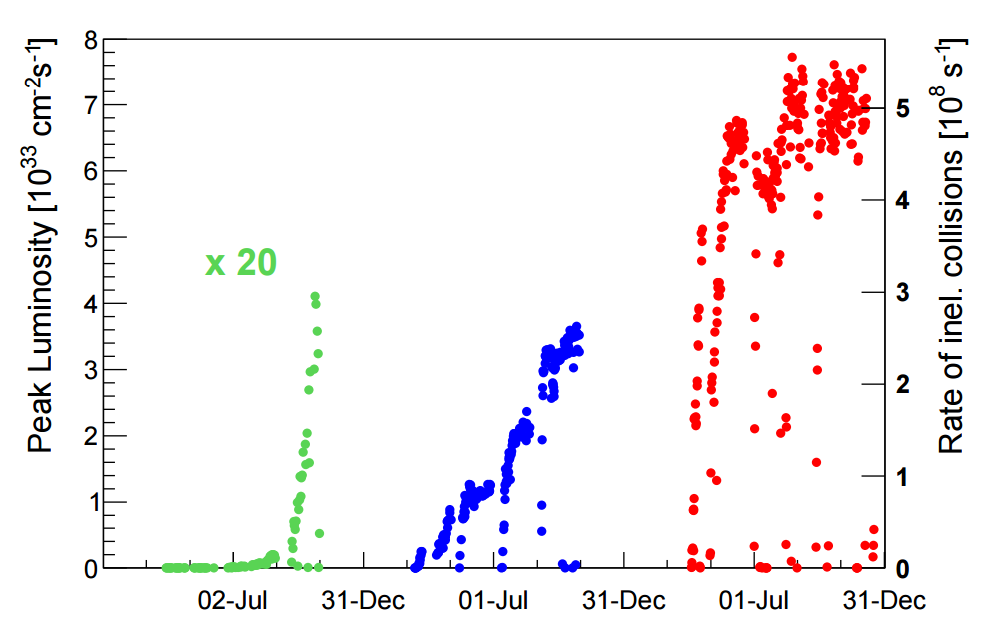
\includegraphics[width=0.5\textwidth]{Figures/LHClumi2.png}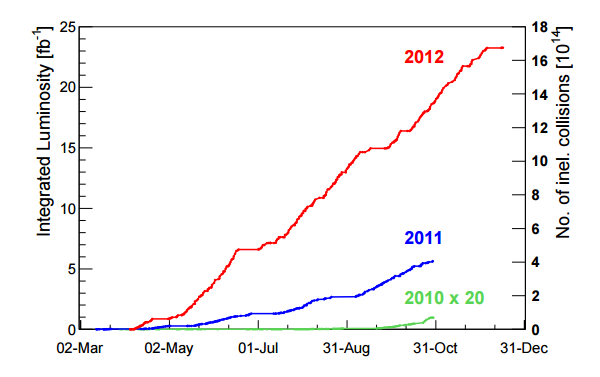
\includegraphics[width=0.5\textwidth]{Figures/LHClumi.png}
\caption{(Left) Peak and (right) integrated luminosity recorded by the LHC between 2010 and 2012 for proton operation. The 2010 luminosity values have been multiplied by a factor 20 \cite{LHClumi}.}
\end{figure}

\begin{figure} \label{fig-CMSlumi}
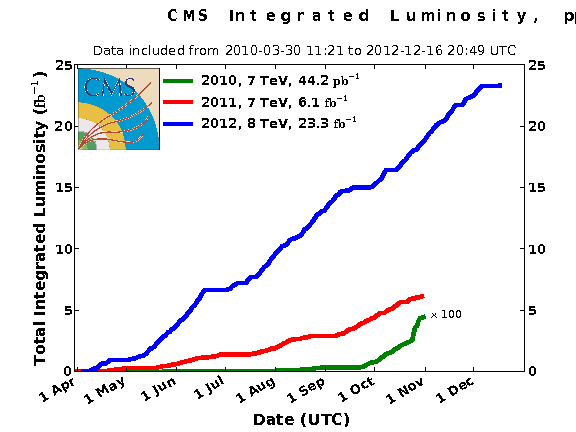
\includegraphics[width=0.5\textwidth]{Figures/IntLumi2.png}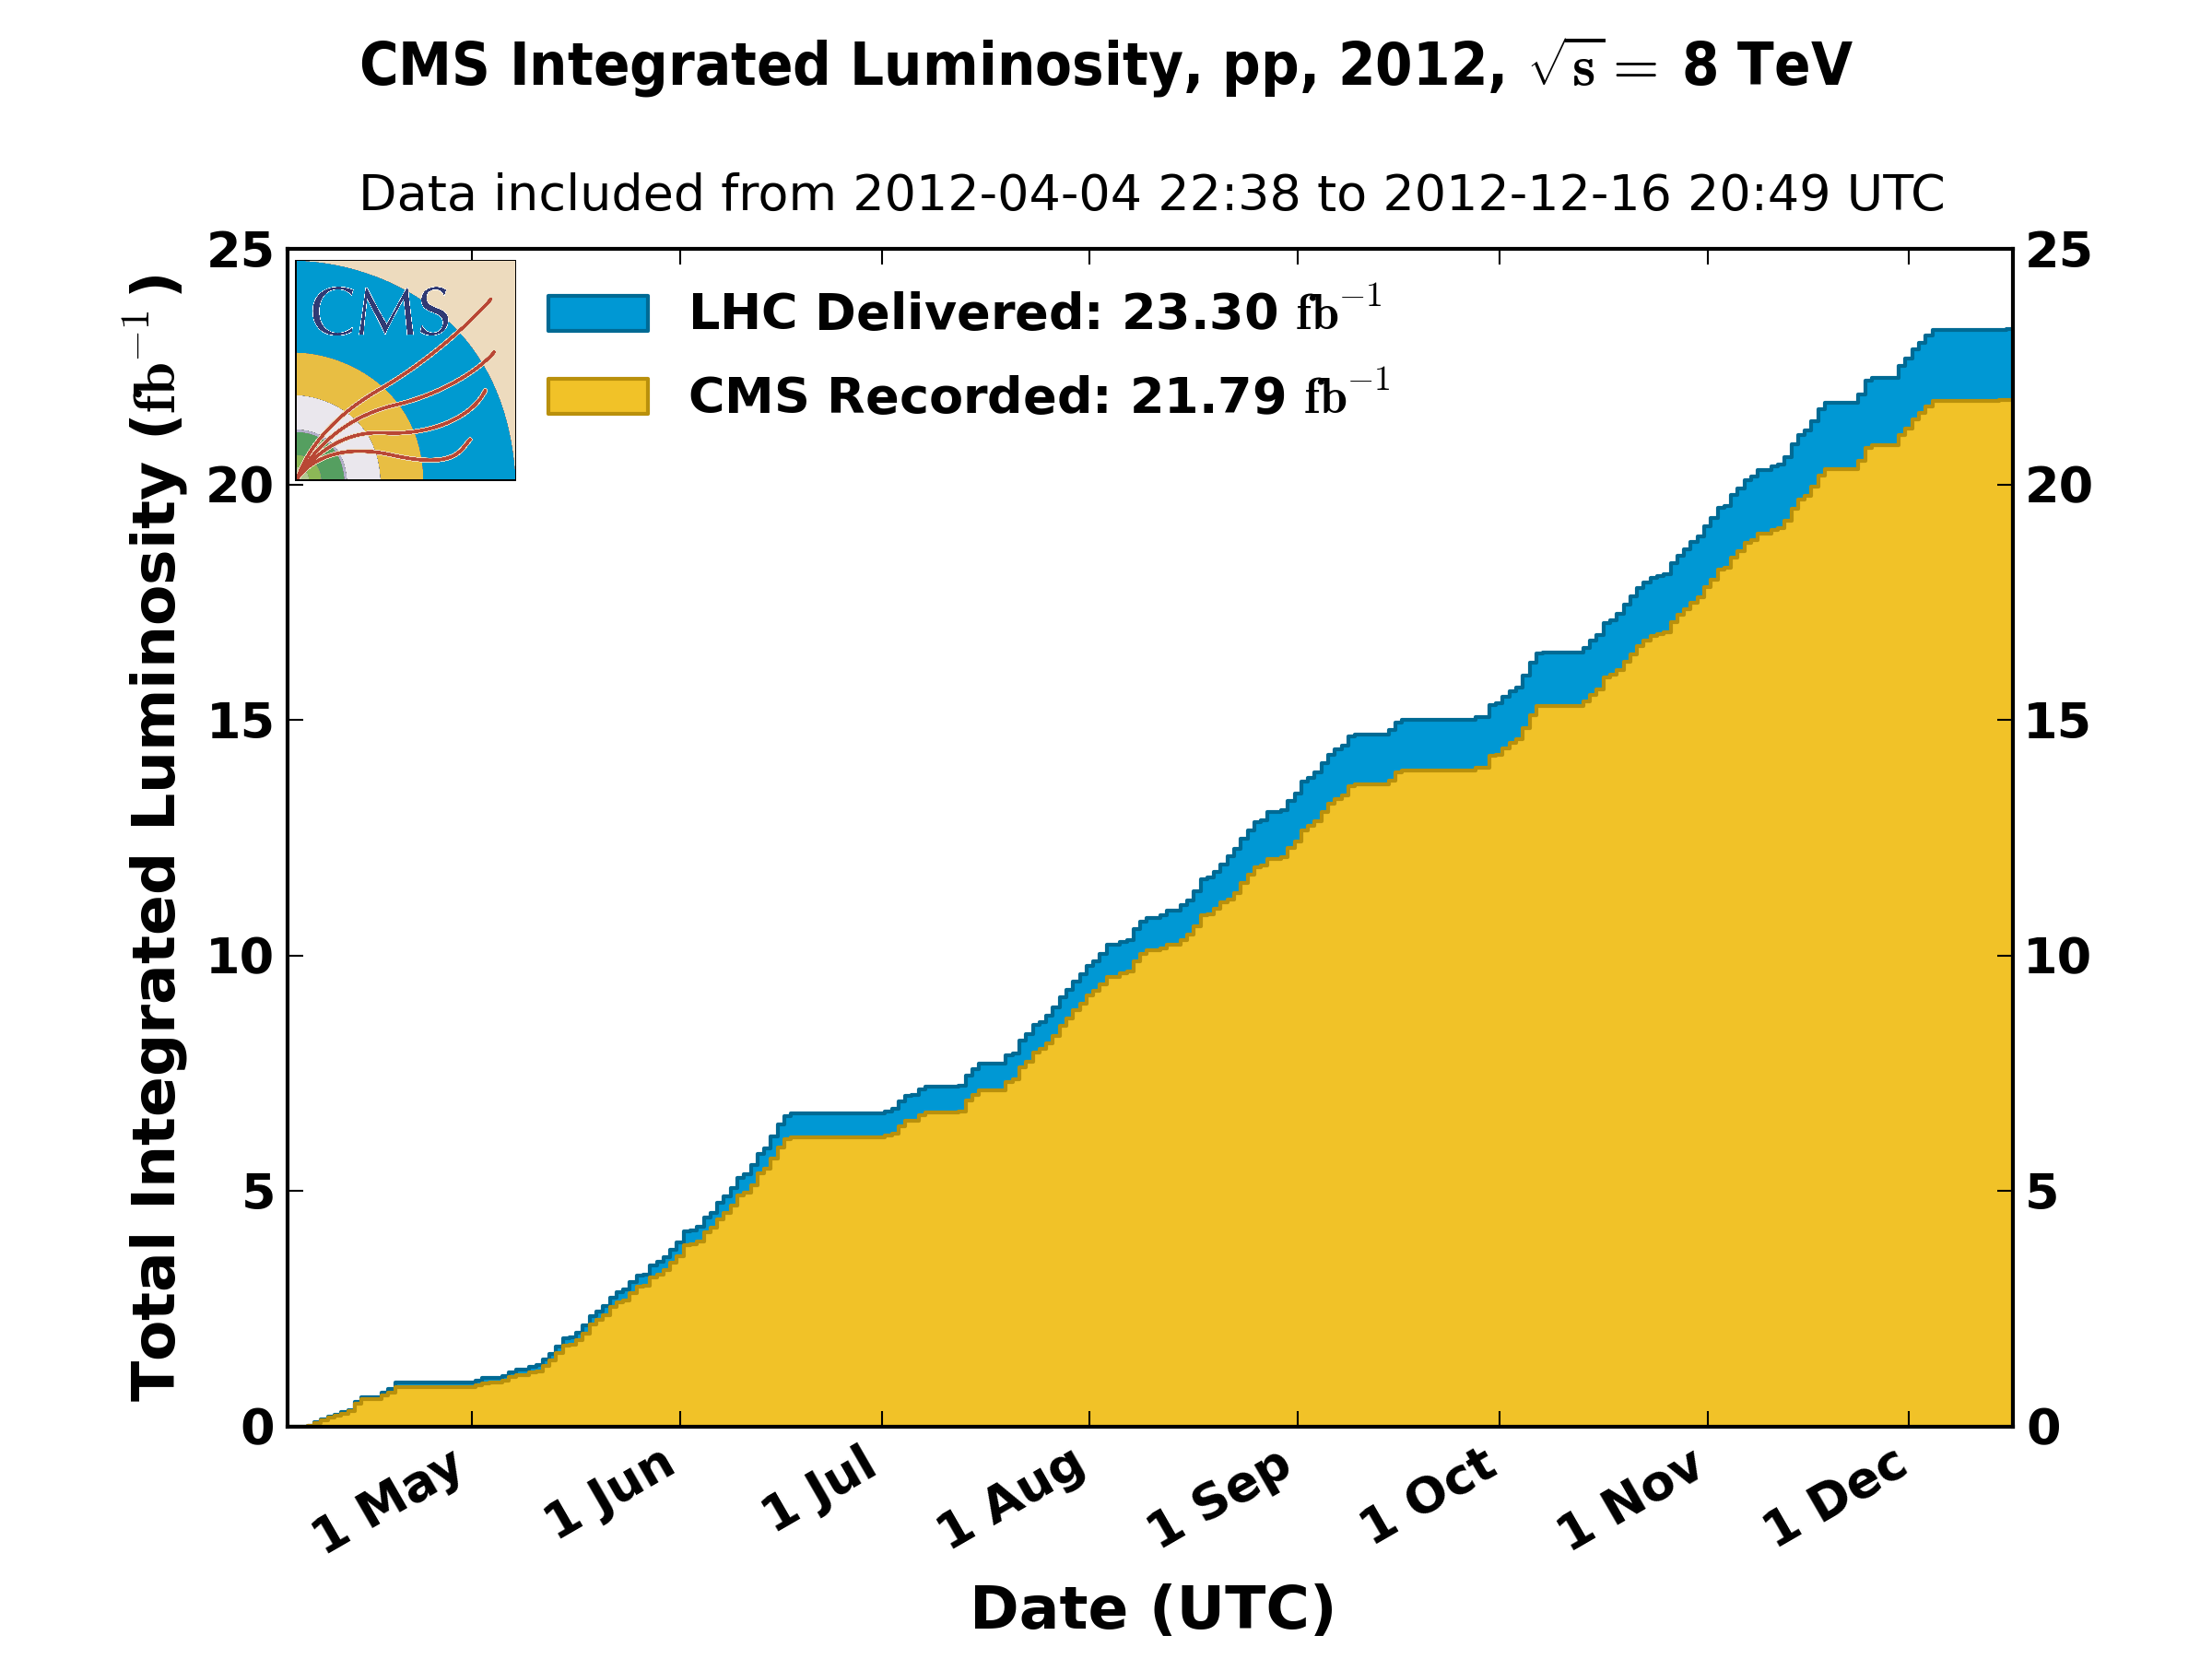
\includegraphics[width=0.5\textwidth]{Figures/CMSIntLumi.png}
\caption{Left: The accumulation of the integrated luminosity produced at the LHC vs time for runs in 2010, 2011, and 2012. The 2010 integrated luminosity is multiplied by 100 in order for it to be visible on the plot. Right: Total integrated luminosity vs time for the 2012 run in CMS and the LHC.}
\end{figure}

\newpage

\section{The CMS Detector} \label{sec-TheCMSDetector}

\begin{figure} [h!] \label{fig-CMSDetector}
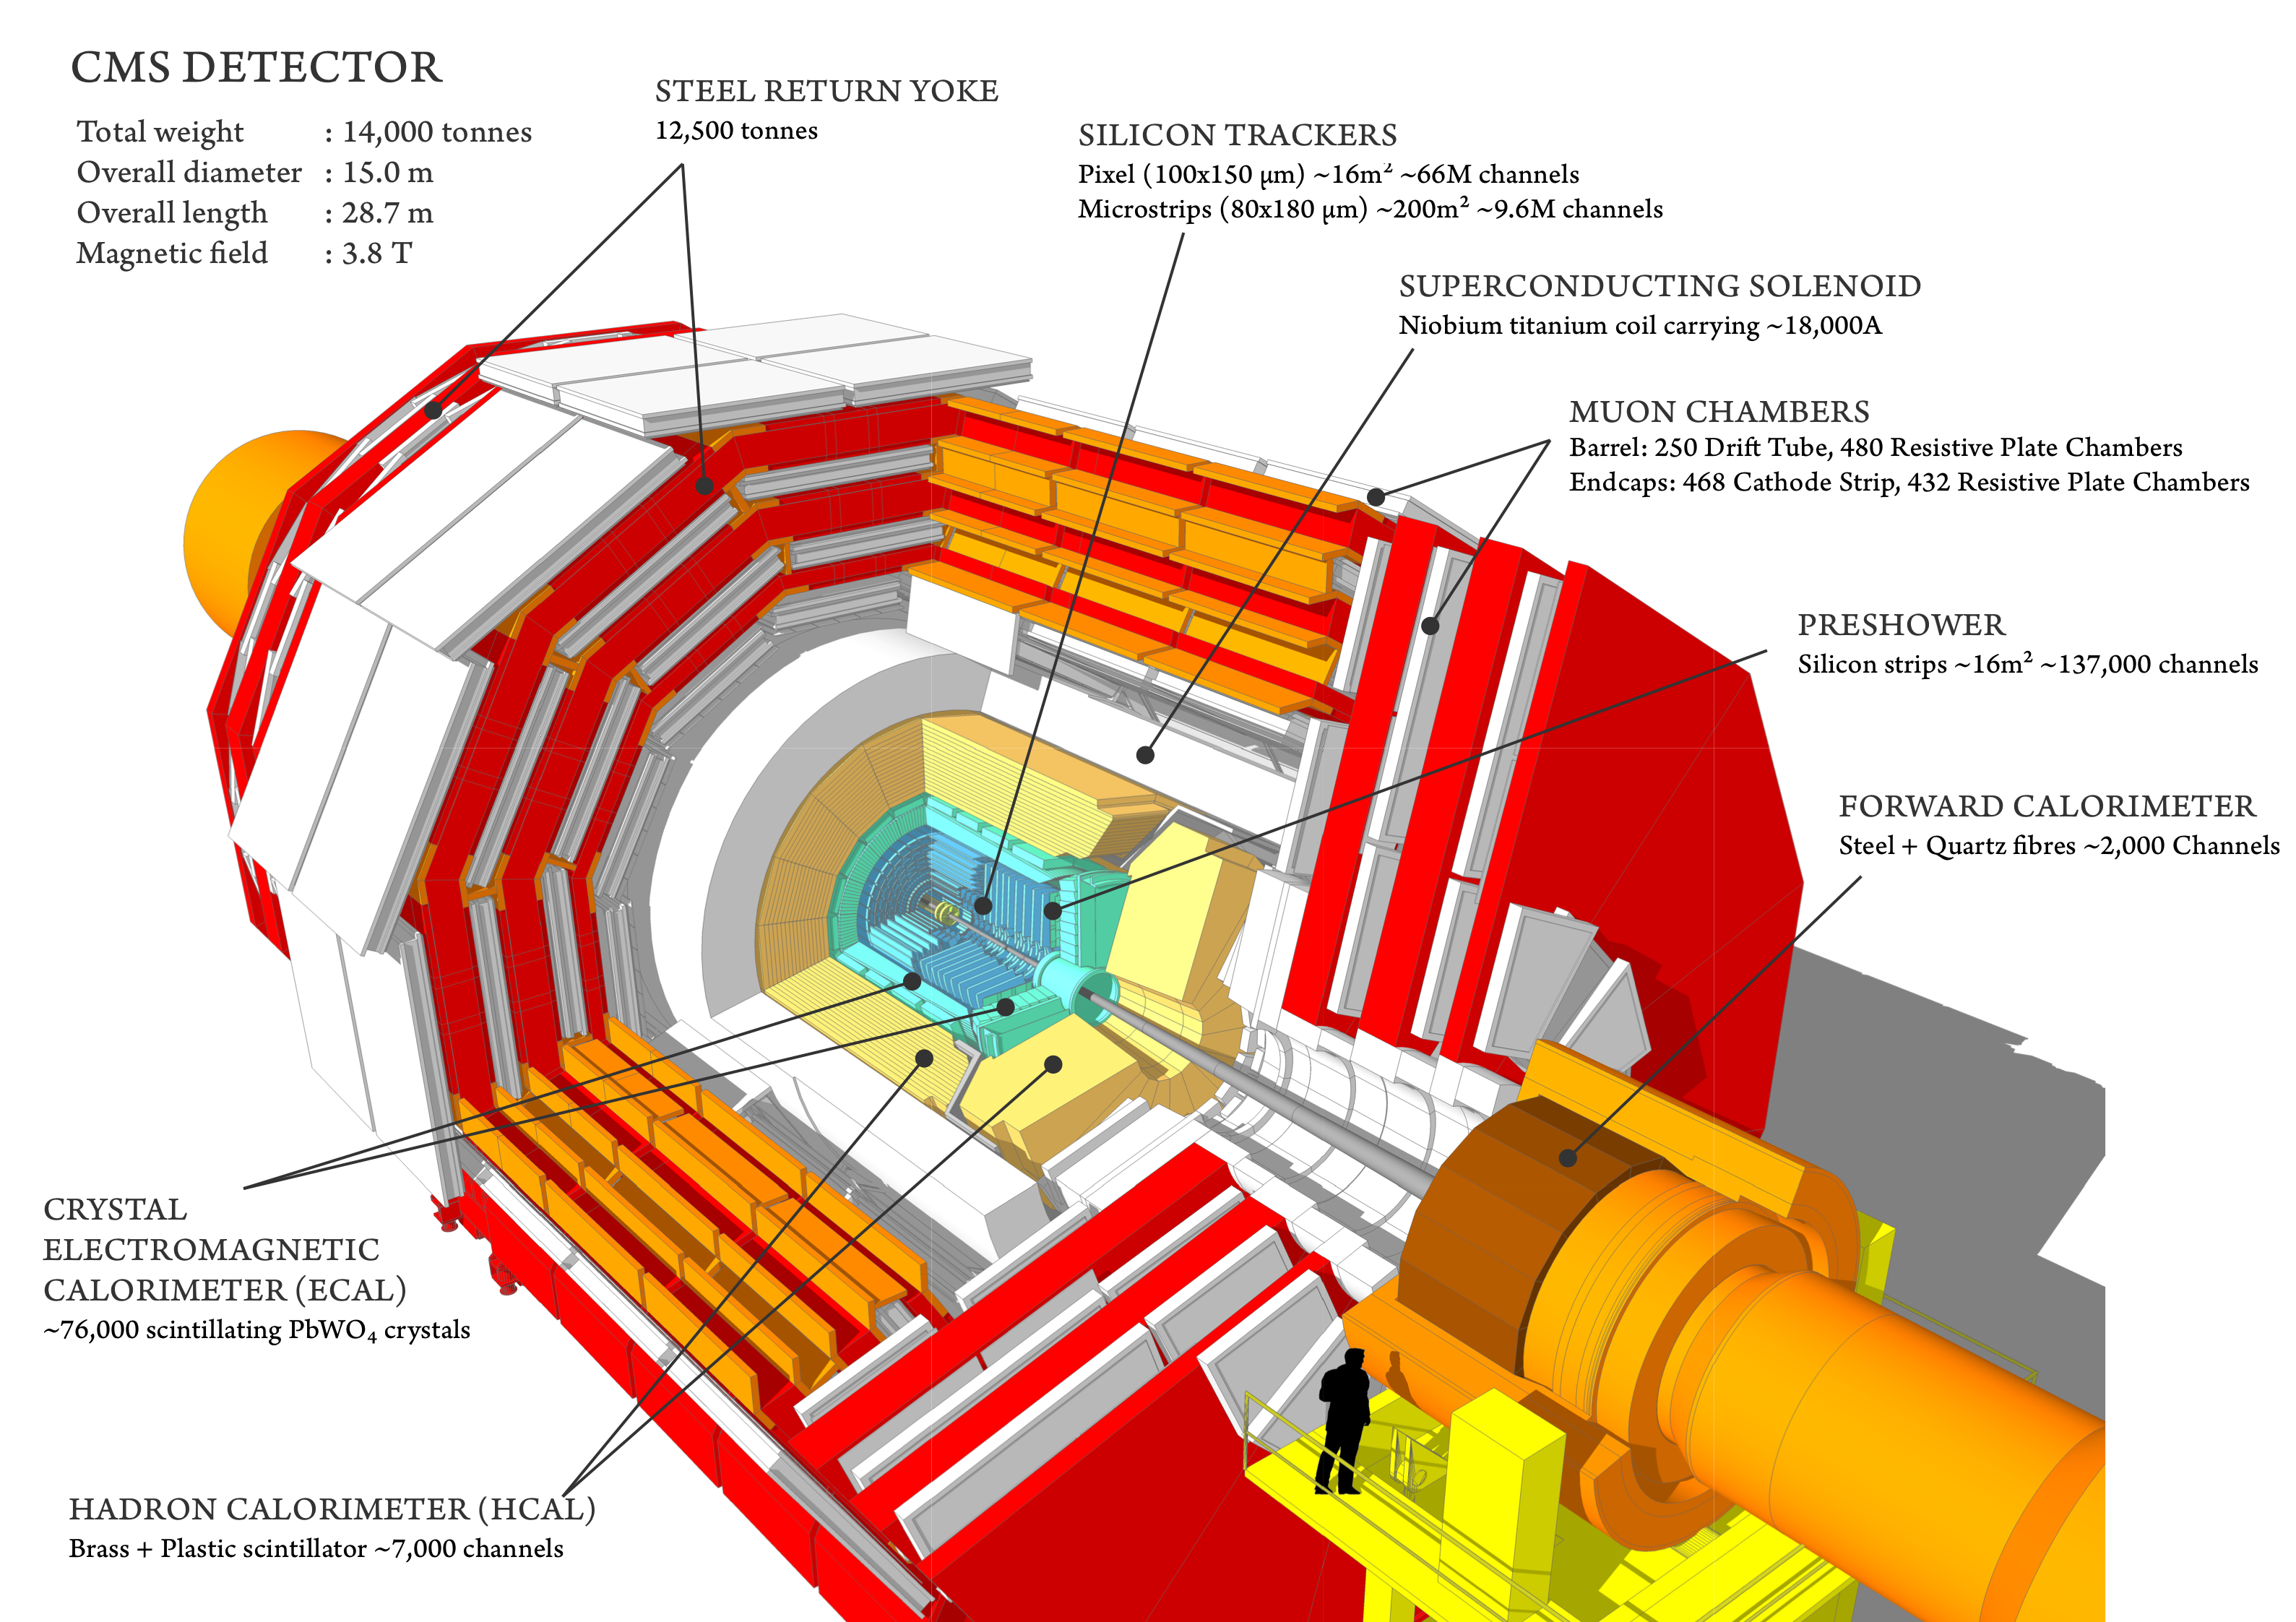
\includegraphics[width=\textwidth]{Figures/CMSDetector.png}
\caption{A cross-sectional view of the CMS detector.}
\end{figure}

The Compact Muon Solenoid (CMS) \cite{CMSexperiment} is one of the two all-purpose discovery machines located approximately 100 metres underground at point 5 (Cessy, France) on the LHC ring. Designed to cover the full solid angle, the hermetic detector is composed of multiple sub-detectors, described in detail in the following sections, designed to to perform precision particle detection and withstand extremely high doses of radiation. Unlike the other detectors that lie on the LHC ring CMS is designed with the purpose of precision measurements of Standard Model measurements and the discovery of physics beyond that of the Standard Model. The primary physics motivation for the construction of such a detector was to elucidate the nature of electroweak symmetry breaking of which the Higgs field was theorised to be responsible, which was proved correct in 2012 with the discovery of the quanta that propagates the Higgs field - the Higgs boson. Many theories predict to observe new physics at the TeV scale, and so CMS was designed with the intention to be able to withstand high energy and fluence of particles. Discovering physics beyond the Standard Model would pave the way for a potential unified theory. The detector weighs around 14,000 tonnes and has an overall length of 28.7 metres and diameter of 15 metres. A sectional view of the CMS detector labeling each sub-detector within is shown in Figure \ref{fig-CMSDetector}. CMS uses a right-handed coordinate system whereby the x-axis points towards the center of the LHC ring, the y-axis lies perpendicular to the beam, and the z-axis follows the direction of the beam anti-clockwise. The azimuthal angle, $\phi$, is measured from the x-axis in the xy plane where the radial component in this plane is define by r, and the polar angle $\theta$ in the rz plane. The pseudorapitiy is thus defined as 

\begin{equation}
\eta = -\ln \left(\tan\left(\frac{\theta}{2}\right)\right)
\end{equation}

and the momentum transverse to the beam is defined as p$_T$, and calculated using the x- and y-components. The transverse energy is defined as E$_T = E\sin\theta$. 

\section{Inner Tracking System} \label{sec-InnerTrackingSystem}

The first sub-detector system located closest to the beam is the Inner Tracking System. The Inner Tracking System is composed of several modules that work in conjunction to provide precise and efficient measurements of the trajectories of charged particles resulting from the beam collisions, as well as a precision reconstruction of secondary vertices, whereby the product from the LHC beam collision decays. The tracker is completely hermetic around the interaction point (IP) of the beam-line, is 5.8 m in length, and has a diameter of 2.5 m. In order to reconstruct particle tracks momentum measurements must be made. To do this the tracker works in combination with the CMS Superconducting Solenoid (Section \ref{sec-SuperconductingSolenoid}) with a magnetic field at 4 T. 

Due to the high flux of the LHC at design luminosity the inner tracker will receive around 1000 particles per bunch crossing with around 20 primary vertices per collision, therefore the tracker was designed to operate with a high granularity and fast response time such that trajectories can be precisely identified and associated with the correct bunch crossing. Several challenges arise upon implementation of such technology: the requirement of high power density to the on-detector electronics means that sufficient cooling must be used throughout, which then conflicts with the ideology of keeping material to a minimum to prevent effects such as multiple scattering, bremsstrahlung, photon conversion, and nuclear scattering. Another challenge presents itself in the form of radiation damage to the tracking system due to the large flux of high energy particles over time. The requirements for a high granularity detector using minimum material that can run over a period of roughly 10 years whilst remaining radiation hard lead to a final design entirely based on silicon detector technology. 

Shown in Figure \ref{fig-Tracker}, the Inner Tracking System is composed of a pixel detector with a radii of between 4.4 cm and 10.2 cm, and a silicon strip tracker which in composed of 10 barrel detection layers reaching a radius of 1.1 m. In order to make tracking system completely hermetic the barrel detectors are surrounded by endcaps composed of 2 disks in the pixel detector and 3 plus 9 disks of silicon strip tracker, thus extending the acceptance, $A$, of the tracker up to a pseudorapidity of $|\eta| < 2.5$.  Each individual pixel station covers a region of $100\times150$ $\mu$m$^2$ in the $r-\phi$ and $z$ coordinate system, respectively, and is driven by the desired impact parameter resolution. In total the pixel detector contains 66 million pixels, corresponding to an active area of 1 m$^2$.

\begin{figure} [h!] \label{fig-Tracker}
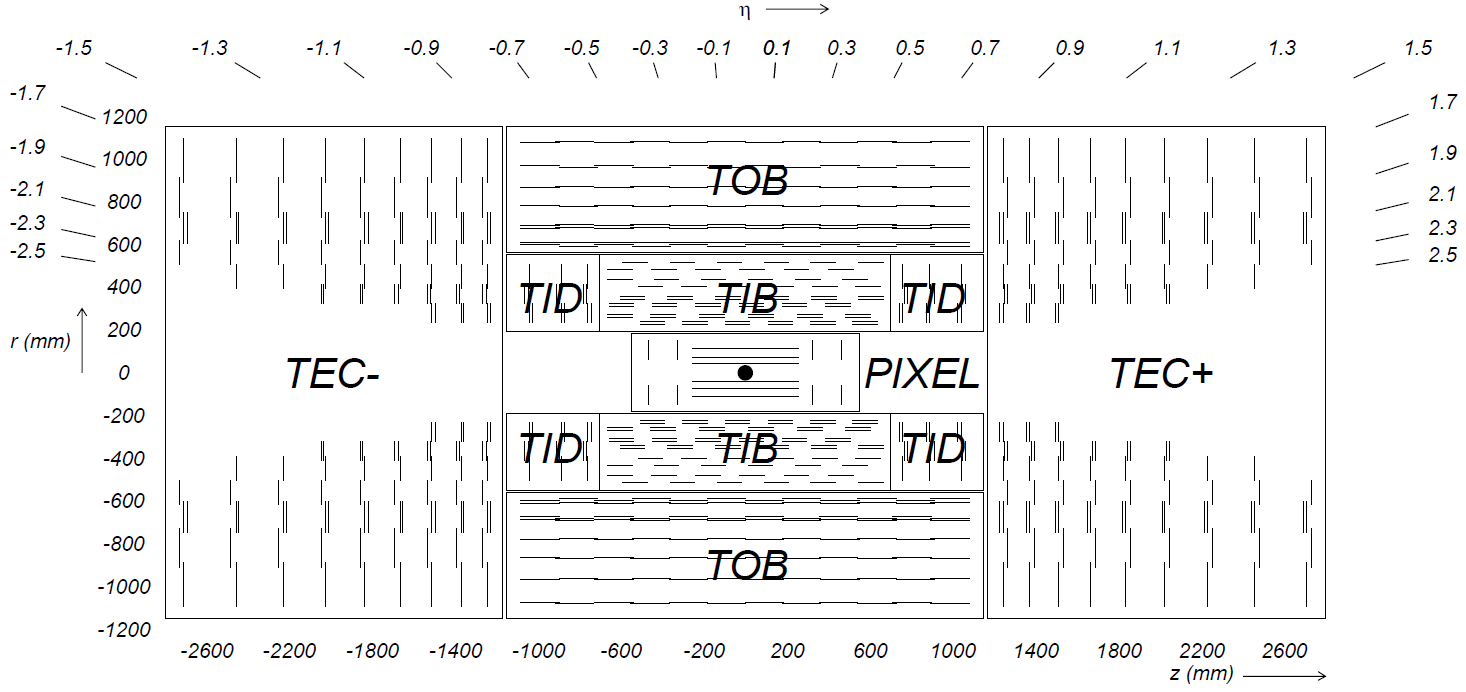
\includegraphics[width=\textwidth]{Figures/Tracker.png}
\caption{The sub-detectors of the CMS silicon tracker system: TOB=outer barrel, TIB=inner barrel, TID=inner disc, TEC=endcaps, PIXEL=pixeldetector. Each line represents a detector module. Double lines indicate back-to-back modules which deliver stereo hits. \cite{CMSexperiment}.}
\end{figure}

The sensor elements in the silicon strip tracker system are single sided p-on-n type silicon micro-strip sensors \cite{SiliconStripSensors1,SiliconStripSensors2}. The Tracker Inner Barrel (TIB) and Disks (TID), where the particle flux is smaller, extends to a radius of between 20 cm $< r <$ 55 cm, and has a typical cell size of 10 cm $\times 80 \mu$m$^2$, strip thickness of $320 \mu$m, and an occupancy of $\sim2-3\%$ per strip per bunch crossing. The outer layer of the silicon strip tracker ranges from 55 cm $< r <$ 110 cm and $\sim500 \mu$m thick, but with a cell size of 25 cm $\times$ 180 $\mu$m due to lower levels of radiation in the outer region. The TIB and TID are surrounded by the Tracker Outer Barrel (TOB) which has an outer radius of 116 cm and comprises 6 barrel layers of 500 $\mu$m thickness micro-strip sensors and strip patches of 183 $\mu$m on the first 4 layers and 122 $\mu$m on the 5th and 6th layers. Beyond the range of the TOB lies the Tracker EndCaps (TEC+ and TEC-, where the sign represents the location of the endcap along the z-axis) to provide complete coverage. The TECs cover the region 124 cm $<|z|<$ 282 cm and 22.5 cm $<|r|<$ 113.5 cm and is composed of 9 disks each consisting of 7 rings of silicon micro-strip detectors, 320 $\mu$m thick on the inner 4 rings, 500 $\mu$m thick on rings 5-7) with radial strips of 97 $\mu$m to 184 $\mu$m average pitch. Therefore, they provide up to 9 $\phi$ measurements per trajectory.

\subsection{Tracker performance in Run I} \label{subsec-TrackerPerformance}

Over the Run I period, from 2010 to 2013, the LHC delivered around 6 fb$^{-1}$ at 7 TeV and 23.3 fb$^{-1}$ at 8 TeV (Figure \ref{fig-LHClumi}), out of this approximately 93\% was recorded by CMS. The CMS tracker was responsible for roughly one third of the lost data due to the high voltage only being ramped up once stable beams are reached. By the end of Run I approximately 2.3\% of the tracker barrel and 7.2\% of the endcap modules were inactive associated with faulty wire-bonds or poor connections. During this period around 2.5\% of the strip detector became inactive because of short-circuits in the control rings and HV lines, or due to faulty optical communications. Maintenance and repairs began upon shutdown of the LHC, and CMS was able to salvage up to 1.5\% of the pixel barrel, up to 0.5\% of the pixel endcap modules, and up to 1\% of the strip detectors \cite{TrackerPerformance}.

In order to process the data prior to track reconstruction the hit efficiency must be measured, the points at which a charged particle traversed each layer of the inner tracker. After track reconstruction the efficiency is calculated as the fraction of particles that are expected to pass through the fiducial regions of the sensors in a layer of the detector in which matching hits are found. For the strip detectors a hit is considered to be a hit if the energy deposit is found in the module in which it was expected to be observed. For efficient reconstruction of tracks knowledge of the position of each module in three-dimensional space is required. Distortions and movements of the inner tracker modules were monitored using cosmic ray data and collision tracks by measuring the distance between expected and observed track trajectories. Distortions in tracking lead to biases in the reconstructed track curvature, and were studied using the reconstructed mass of $Z \to \mu\mu$ events as a function of the positive muon's azimuthal angle. The muon reconstruction efficiency can be seen in Figure \ref{fig-MuonReconstructionEfficiency}.

\begin{figure} \label{fig-MuonReconstructionEfficiency}
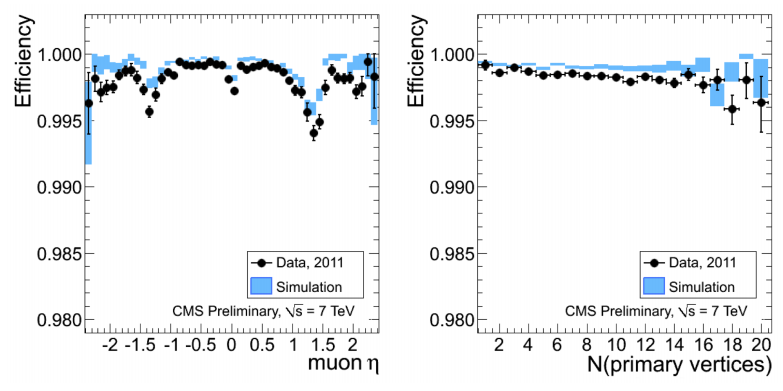
\includegraphics[width=\textwidth]{Figures/MuonReconstructionEfficiency.png}
\caption{Muon reconstruction efficiency in thee tracker as functions of pseudorapidity (left) and the number
of proton-proton interaction vertices (right) \cite{TrackingResults}.}
\end{figure}

\begin{figure} \label{fig-PVResolution}
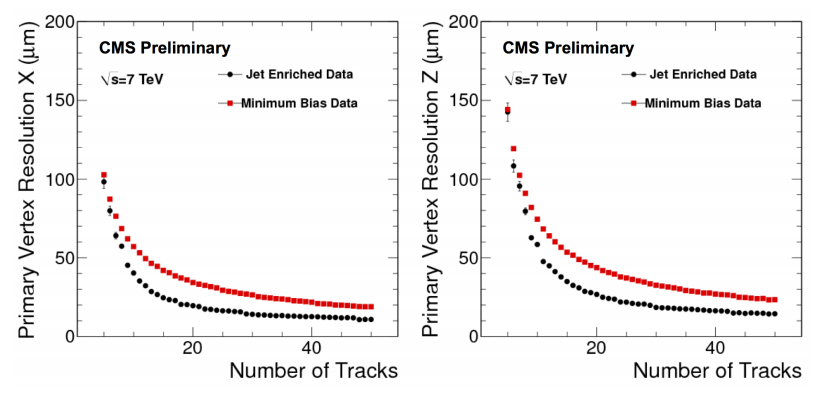
\includegraphics[width=\textwidth]{Figures/PVResolution.png}
\caption{Primary vertex resolution in the transverse plane (left) and along the beam-line (right) as functions
of the number of tracks attached to the vertex \cite{TrackingResults}.}
\end{figure}

The CMS tracking software relies on an iterative procedure to measure hits in a high particle occupancy environment. Earlier steps of the tracking process search for tracks with higher p$_T$ due to the more obvious nature of the tracks, which include a smaller impact parameter, and greater number of measured hits in each layer of the tracker. By selecting more obvious processes first, the reconstruction becomes easier as it has fewer events to deal with. Track reconstruction efficiency is measured by using the tag and probe method in $Z \to \mu\mu$ events \cite{TrackingResults}. The tracking efficiency is then defined as the number of probes observed to have matching tracks within the tracker and is a function of the number of primary vertices and the pseudorapidity of the tracks and can be seen in Figure \ref{fig-PVResolution}. LHC proton-proton events are reconstructed by firstly identifying the tracks, then grouping in accordance with their primary vertex, and finally fitting to the position of each vertex.  

One of the long term damaging effects of high luminosity collisions is radiation damage. Radiation damage in the silicon was monitored throughout Run I and tested by performing special runs where the bias voltage was increased in steps from 0 to the operational voltages. Results showed that the hit efficiency decreased with irradiation at first, then increased with changes in the effective doping \cite{Doping}. Due to collisions not being completely aligned at the centre of the detector, even irradiation of the modules is seen in the azimuthal direction.

Overall, the CMS tracker has performed exceptionally throughout the Run I three-year period with regards to detector reliability and tracking. The tracker was able to overcome a major problem of high pile-up and reconstruct tracks with excellent efficiency. Less than 3\% of the tracker became inactive throughout the entire run, and less than 5\% of the delivered luminosity was lost through the tracker.    
 
\section{Electromagnetic Calorimeter} \label{sec-ElectromagneticCalorimeter}

\subsection{Overview} \label{subsec-ECALOverview}

Directly after the Inner Tracking System, the second stage of particle identification and reconstruction comes in the form of the Electromagnetic Calorimeter (ECAL). The ECAL serves to stop electromagnetic particles, namely electrons and photons, and measure the energy deposited in the detector. These particles are identified and reconstructed using signatures such as charge, shower shape, and isolation. When an electron passes through the ECAL it showers via bremsstrahlung. Radiation losses due to bremsstrahlung scale with mass as m$^{-4}$ (m$^{-6}$) when a charged particle travels perpendicular (parallel) to an electric field, and thus heavier electromagnetic particles are less likely to produce a shower. It is possible to differentiate between electrons and positrons by the curvature produced from the Superconducting Solenoid. Photons are neutrally charged and thus do not bend via the magnet, however they produce a shower of electron-positron pairs which can then be measured. The photon shower shape, known as $\sigma_{i\eta i\eta}$, is a prominent variable in this analysis and will be described in detail in Section \ref{sec-}.  

A key component that drove the design of the ECAL is the decay channel $H \to \gamma\gamma$. At the time of design, the Higgs had not been discovered and thus the mass was not known, however it was known that the aforementioned decay mode was sensitive to a low mass Higgs, $m_H<150$ GeV. Although the branching ratio of the decay is small ($\simeq0.002$), the signature is clean and is a narrow resonance of two high E$_T$ photons over a non resonant background \cite{HiggsProposal}. In order to discover the Higgs the detector needed to have a powerful invariant mass resolution and background rejection, translating into a need for extremely efficient photon and electron identification, along with a high position and energy resolution. 

\subsection{Composition of the ECAL} \label{subsec-ECALComposition}

The CMS ECAL is a is a hermetic, homogeneous fine-grained lead tungstate (PbWO$_4$) crystal calorimeter \cite{ECAL}, shown in Figure \ref{fig-ECAL}. The PbWO$_4$ crystals are extremely dense  ($\delta=8.28$ g/cm$^3$), thus providing excellent performance and compactness, and thus fit within the Superconducting Solenoid magnet volume. The crystals were designed with an extremely small radiation length, $X_0=0.85$ cm, and small Moli\`{e}re radius, $R_M=2.19$ cm. The decision to use a homogeneous medium was chosen because of the ability to obtain a greater energy resolution by minimizing sampling fluctuations \cite{ECAL}. 

\begin{figure} [h!] \label{fig-ECAL}
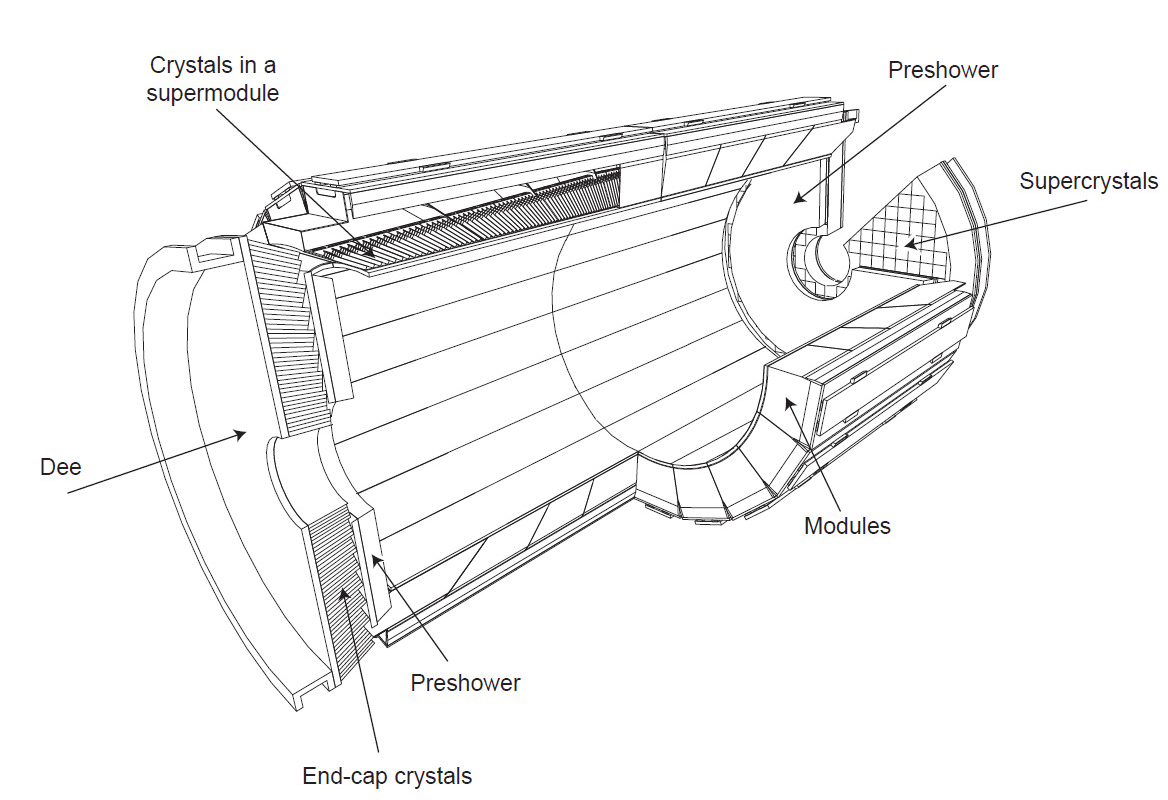
\includegraphics[width=\textwidth]{Figures/ECAL.png}
\caption{Geometric view of one quarter of the ECAL (top). Layout of the CMS electromagnetic calorimeter presenting the arrangement of crystal modules, supermodules, endcaps and the preshower in front (bottom) \cite{CMSexperiment}.}
\end{figure}

There are 75,848 within the ECAL, and are arranged into a barrel section (EB), covering a pseudorapidity rang of $|\eta|<1.4442$, which is then surrounded by endcaps and thus extending the pseudorapidity range to $|\eta|<3.0$. The length of the crystals within the barrel are 230 mm and 220 mm in the endcap regions, which corresponds to $\sim26$ (EB) and $\sim25$ (EE) radiation lengths. The crystals are projective and also slightly off-pointing in position, $\sim3^\circ$ with respect to the IP. This configuration provides a full coverage and ensures that there are no cracks in the calorimetry that are aligned with particle trajectories. Within the barrel there is no longitudinal segmentation, and therefore the angle at which a photon is measured relies on the reconstructed PV from the silicon tracker. EB crystals are $2.2\times2.2$ cms$^2$ on the front face, and $2.86\times2.86$ cm$^2$ in the endcaps, giving rise to a total crystal volume of 11 m$^3$ and a weight of 92 t.

The barrel crystals are arranged into 36 supermodules (or superclusters), each containing 1,700 crystals, whereas the endcaps are arranged into two D-shaped segments comprising 3,662 crystals each. The final section of the ECAL is the pre-shower detector system (ES) placed directly in front of the endcaps at $1.65<|\eta|<2.6$ and can be visualised in Figure \ref{fig-ECALRapidity}. The ES is composed of 4,288 sensors, 137,216 silicon strip sensors, each $1.90\times61$ mm$^2$ with x-y view, and has a total of $\sim3$ radiation lengths. The purpose of the ES is provide improved separation of photons to $\pi^0$s.

\begin{figure}\label{fig-ECALRapidity}
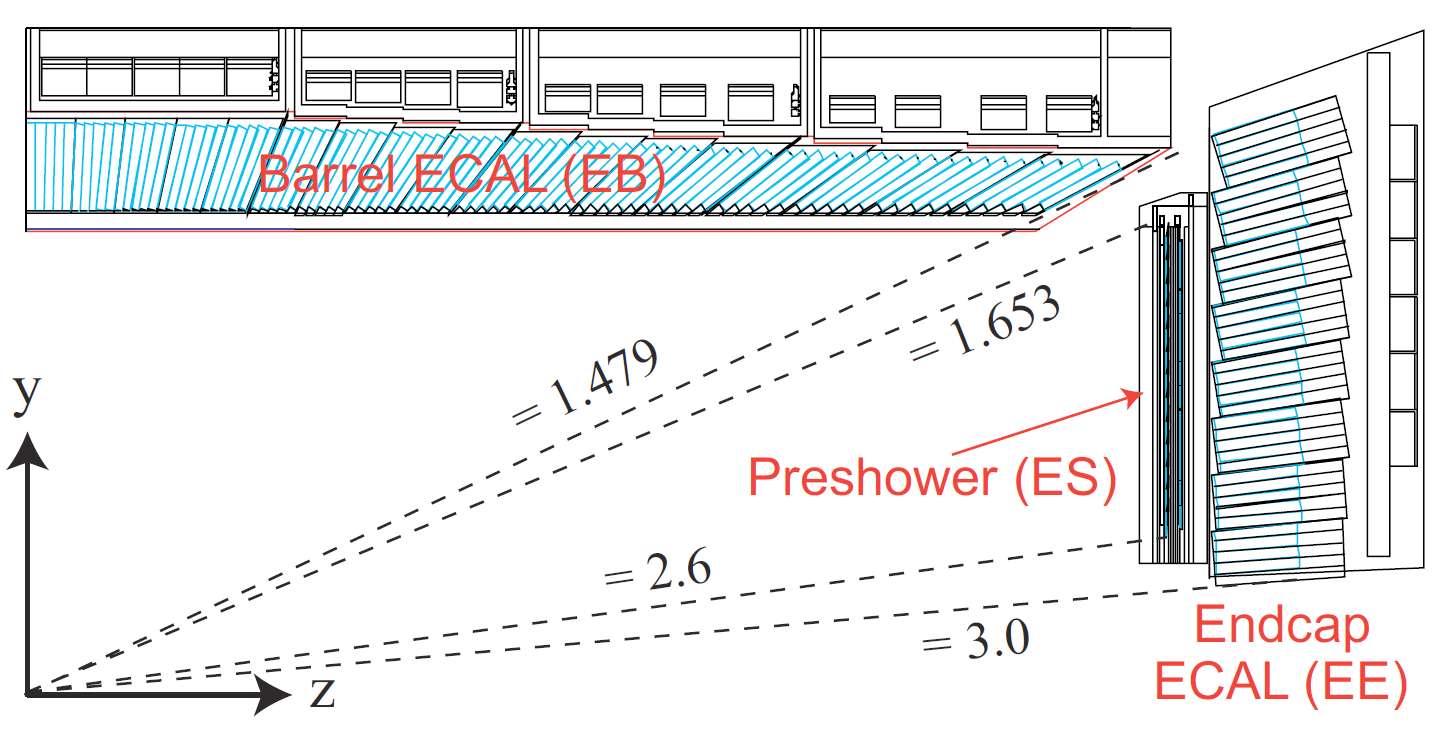
\includegraphics[width=\textwidth]{Figures/ECALRapidity.png}
\caption{Geometric view of one quarter of the ECAL (top). Layout of the CMS electromagnetic calorimeter presenting the arrangement of crystal modules, supermodules, endcaps and the preshower in front (bottom) \cite{CMSexperiment}.}
\end{figure}

\subsection{Photodetectors} \label{subsec-Photodetectors}

The light read-out system for the barrel crystals comes in the form of Hamamatsu avalanche photodiodes (APD). There are two APDs for each crystal which are read in parallel, each measuring $5\times5$ mm$^2$ with a quantum efficiency (QE) of 75\%. The gain is set at $\sim50$ and they are insensitive to the 4 T magnetic field from the Superconducting Solenoid. The endcap crystals scintillation light is read out by vacuum photo-triodes (VPT), each with an area of 280 mm$^2$ with a 20\% QE and gain of $\sim10$. The barrel APDs are temperature sensitive ($\frac{1}{E}\frac{dE}{dT}\sim-2.3\%C^{-1}$) whereas the VPT sensitivity to temperature is assumed to be negligible relative to that of the crystals.  

\subsection{Performance of the ECAL throughout Run I} \label{subsec-ECALPerformance}

The energy resolution, $\frac{\sigma_E}{E}$ of the ECAL crystals can be parameterised by

\begin{equation}
\left(\frac{\sigma_E}{E}\right)^2 = \left(\frac{A}{\sqrt{E}}\right)^2 + \left(\frac{B}{E}\right)^2 + C^2
\end{equation}

where A and B are the stochastic term for scintillation showers and noise term due to read-out electronics and PMTs, respectively. C is a constant term which is a direct measure of the performance of the PbWO$_4$ crystals. 

\begin{figure} \label{fig-}
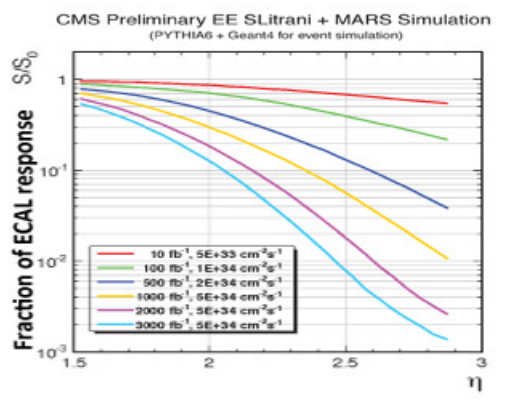
\includegraphics[width=0.48\textwidth]{Figures/EEFractionalResponse.png}
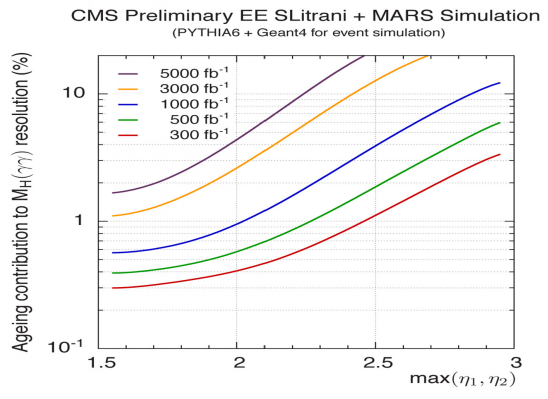
\includegraphics[width=0.52\textwidth]{Figures/EEResolutionDeterioration.png}
\caption{Simulation of fractional response from EE as a function of $\eta$, for different integrated luminosities. Right: Deterioration of the energy resolution in EE as a function of $\eta$, for different integrated luminosities \cite{ECALPerformance}.}
\end{figure}

\section{Hadron Calorimeter} \label{sec-HadronCalorimeter}

\section{Superconducting Solenoid} \label{sec-SuperconductingSolenoid}

The CMS Superconducting Solenoid, shown in Figure \ref{fig-SuperconductingSolenoid}, is the most powerful magnet in the world, 100,000 times stronger than the Earth's magnetic field and stores enough energy to melt 16 tonnes of gold, and the most essential feature of the detector. In order to achieve a good momentum resolution in such a detector, without making tight cuts on muon chamber resolution and alignment, a powerful magnetic field was chosen. A large bending power can be achieved by a modestly sized solenoid, as long as it is a high-field superconducting one, due to the bending beginning at the primary vertex. The requirement for the bending power of the solenoid is dictated by the narrow states decaying into muons, and by the unambiguous determination of the sign for muons with a momentum of around 1 TeV/c. In order to obtain a precision measurement, a momentum resolution of $\Delta p/p\approx10\%$ at p = 1 TeV/c. A suitable length to radius ratio is required to obtain a good momentum resolution in the forward region, and can be seen in the parameters listed in Table \ref{tab-SolenoidParameters} \cite{PTDR2}. 

\begin{table} \label{tab-SolenoidParameters}
\begin{center}
\begin{tabular}{|l|c|}
\hline
	\multicolumn{2}{|c|}{\textbf{Superconducting Solenoid Parameters}} \\
\hline
	\textbf{Parameter} & \textbf{Value} \\
\hline
	Field (T) & 4 \\
	Length (m) & 12.9 \\
	Weight (t) & 250 \\
	Inner bore (m) & 5.9 \\
	Current (kA) & 19.5 \\
	Number of turns & 2168 \\
	Stored energy (GJ) & 2.7 \\
	Hoop stress (atm) & 64 \\
\hline
\end{tabular}	
\caption{Parameters of the LHC superconducting solenoid \cite{MagneticField}.}
\end{center}
\end{table}

Approaching 13 m in length, and 6 m in diameter, the solid mass weights approximately 250 t at an operating temperature of $-268.5^\circ C$ -- a degree warmer than outer space. Originally designed to run with a uniform magnetic field of 4 T within the 5.9 m bore, the eventual operating level was set to 3.8 T in order to increase the lifetime. Such a magnetic field requires a return yoke, which can be viewed in the CMS schematic in Figure \ref{fig-CMSDetector}, of which the return field is large enough to saturate 1.5 m of iron and weighs 12,500 t. This allows four muon stations to be integrated within the return yoke, ensuring robustness and full geometric coverage. The magnet and return yoke use almost twice as much iron as the Eiffel Tower.

\begin{figure} \label{fig-SuperconductingSolenoid}
\begin{center}
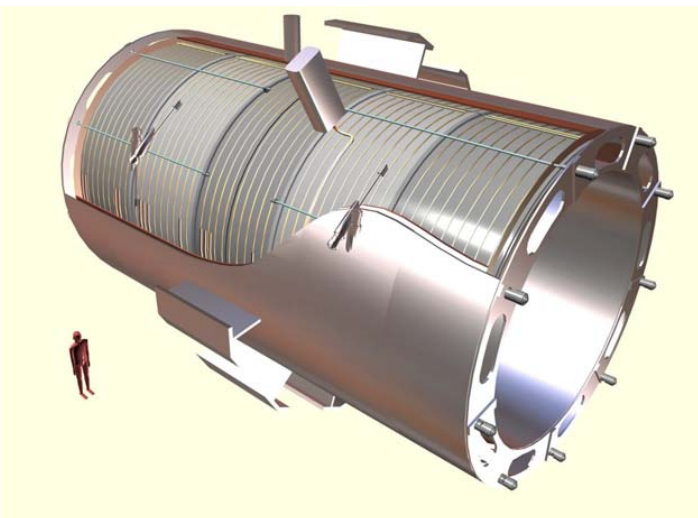
\includegraphics[scale=0.5]{Figures/SuperconductingSolenoid.png}
\caption{ General artistic view of the 5 modules composing the cold mass inside the cryostat, with details of the supporting system (vertical, radial and longitudinal tie rods) \cite{CMSexperiment}.}
\end{center}
\end{figure}


\section{Muon System} \label{sec-MuonSystem}

CSCs
RPCs
DTs

\begin{figure}\label{fig-CMSLongitudinalView}
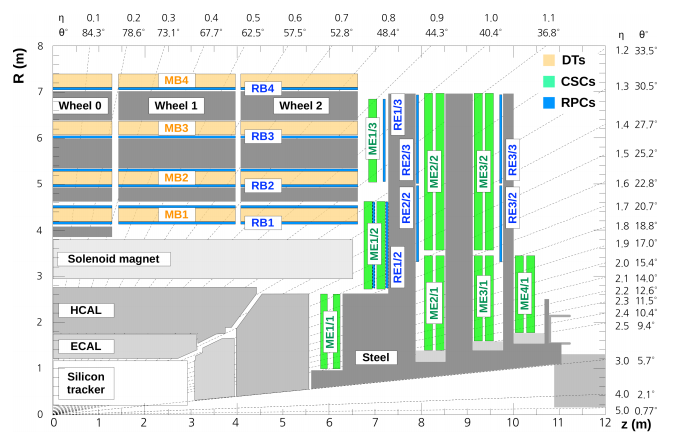
\includegraphics[width=\textwidth]{Figures/CMSLongitudinalView.png}
\caption{Layout of one quadrant of CMS. The figure shows the four DT stations in the barrel (MB1-MB4, yellow), the four CSC stations in the endcap (ME1-ME4, green), and the RPC stations (RB1-RB4 and RE1-RE3) \cite{CMSexperiment}.}
\end{figure}

\section{Trigger} \label{sec-Trigger}

At design energy, the total proton-proton cross-section is expected to be approximately 100 mb, and should therefore observe around $10^9$ events/s. This extremely high rate of events leads to numerous experimental and technological challenges, namely the read-out and triggering systems. There will be roughly 20 inelastic events that will be superimposed onto events that are triggered on, known as pile-up (PU). 

\section{Particle Reconstruction} \label{sec-ParticleReconstruction}

\subsection{Electron identification}

\subsection{Muon reconstruction}

\subsection{Jet reconstruction}

\subsubsection{Jet energy corrections}

\subsubsection{Particle flow jet identification}

\section{Computing}

\subsection{Event Data Model}

\subsection{Analysis Software}

\section{Monte Carlo Simulation}

\begin{sidewaystable} \label{tab-MCSamples}
\begin{center}

\begin{tabular}{|l| p{12.5cm} |c|p{2cm}|}
\hline
	\textbf{Process} & \textbf{Dataset} & \textbf{$\sigma$ (pb)} & \textbf{Number of events} \\
\hline
	$t\bar{t}+\gamma (2\to5)$ & /LHE2EDM\_WHIZARD\_2to5\_ttA/htholen-FULLSIM\_STEP2\_WHIZARD\_2to5\_ttA-da43ae45efb6a7c35e17aad82de2e2cd/USER & 1.8 & 1074860 \\
	$t\bar{t}+\gamma (2\to7)$ & /TTGamma\_TuneZ2star\_8TeV-madgraph-tauola/Summer12\_DR53X-PU\_RD1\_START53\_V7N-v1/AODSIM & 1.8 & 916500\\ 
\hline	
	$t\bar{t}(Leptonic)$ & /TTJets\_FullLeptMGDecays\_8TeV-madgraph/Summer12\_DR53X-PU\_S10\_START53\_V7A-v2/AODSIM & 245.8 & 12119013\\
	$t\bar{t}(Hadronic)$ & /TTJets\_HadronicMGDecays\_8TeV-madgraph/Summer12\_DR53X-PU\_S10\_START53\_V7A\_ext-v1/AODSIM & 245.8 & 31223821\\
	$t\bar{t}(Semileptonic)$ & /TTJets\_SemiLeptMGDecays\_8TeV-madgraph/Summer12\_DR53X-PU\_S10\_START53\_V7A\_ext-v1/AODSIM & 245.8 & 25424818\\
	$t\bar{t}(Inclusive)$ & /TTJets\_MassiveBinDECAY\_TuneZ2star\_8TeV-madgraph-tauola/Summer12\_DR53X-PU\_S10\_START53\_V7C-v1/AODSIM & 245.8 & 6923652\\
\hline	
	Drell-Yann, $10 < m\_{ll} < 50$ & /DYJetsToLL\_M-10To50\_TuneZ2Star\_8TeV-madgraph/Summer12\_DR53X-PU\_S10\_START53\_V7A-v1/AODSIM & 11050.0 & 37835275\\
	Drell-Yann, $m\_{ll} > 50$ & /DYJetsToLL\_M-50\_TuneZ2Star\_8TeV-madgraph-tarball/Summer12\_DR53X-PU\_S10\_START53\_V7A-v1/AODSIM & 3350.0 & 30459503\\
\hline	
	Single Top tW & /T\_tW-channel-DR\_TuneZ2star\_8TeV-powheg-tauola/Summer12\_DR53X-PU\_S10\_START53\_V7A-v1/AODSIM & 11.1 & 497658 \\
	Single TopBar tW $\bar{t}$ & /Tbar\_tW-channel-DR\_TuneZ2star\_8TeV-powheg-tauola/Summer12\_DR53X-PU\_S10\_START53\_V7A-v1/AODSIM & 11.1 & 493460 \\
	Single Top t & /T\_t-channel\_TuneZ2star\_8TeV-powheg-tauola/Summer12\_DR53X-PU\_S10\_START53\_V7A-v3/AODSIM & 56.4 & 99876 \\
	Single TopBar t & /Tbar\_t-channel\_TuneZ2star\_8TeV-powheg-tauola/Summer12\_DR53X-PU\_S10\_START53\_V7A-v1/AODSIM & 30.7 & 1935072 \\
	Single Top s & /T\_s-channel\_TuneZ2star\_8TeV-powheg-tauola/Summer12\_DR53X-PU\_S10\_START53\_V7A-v1/AODSIM & 3.79 & 259961 \\
	Single TopBar s & /Tbar\_s-channel\_TuneZ2star\_8TeV-powheg-tauola/Summer12\_DR53X-PU\_S10\_START53\_V7A-v1/AODSIM  & 1.76 & 139974 \\
\hline	
	W+Jets & /WJetsToLNu\_TuneZ2Star\_8TeV-madgraph-tarball/Summer12\_DR53X-PU\_S10\_START53\_V7A-v2/AODSIM & 36257.2 & 57709905\\
\hline	
	Diboson WW & /WW\_TuneZ2star\_8TeV\_pythia6\_tauola/Summer12\_DR53X-PU\_S10\_START53\_V7A-v1/AODSIM & 56.0 & 10000431\\
	Diboson WZ & /WZ\_TuneZ2star\_8TeV\_pythia6\_tauola/Summer12\_DR53X-PU\_S10\_START53\_V7A-v1/AODSIM & 33.6 & 10000283\\
	Diboson ZZ & /ZZ\_TuneZ2star\_8TeV\_pythia6\_tauola/Summer12\_DR53X-PU\_S10\_START53\_V7A-v1/AODSIM & 8.2 & 9799908\\
\hline	
\end{tabular}
\caption{Dataset information for signal and background MC samples.}
\end{center}
\end{sidewaystable}

\subsection{Monte Carlo event generators}




\chapter{Event Reconstruction \& Simulation} \label{chap-EventReconstruction&Simulation}

Monte Carlo (MC) simulations are an essential part of current particle physics analyses and are used to mimic physical processes that correspond to those which are observed within the LHC, and other such experiments. Analysts compare findings in data to simulation in order to extract signal processes, and also to perform statistical analysis on results obtained. It is of the utmost importance that the simulated events must be as accurate as physically possible in order to mimic real life processes and perform a scientifically accurate analysis. Will talk about methods for generating events, including the different MC generators and tunes used in the evaluation of theoretical uncertainties, and interpretation in terms of the CMS detector in the first section of this chapter.

Roughly speaking, we can divide the different steps of event reconstruction into three separate processes. The first of which records basic information, such as hits within the pixel detectors of the inner tracking system, and calorimeter energy clusters, for `low level' objects in each sub-detector. The information is then passed to the PF algorithm (Section \ref{subsec-PFAlgorithm}) which uses information from all the sub-detectors in order to reconstruct events much more accurately. Finally, the events are refined by other complex statistic and mathematical techniques and used to reconstruct higher level objects, such as jets and MET. The second part of chapter will focus on the PF process \cite{CMS-PAS-PFT-09-001, CMS-PAS-PFT-10-001} as mentioned above.

\section{Event Reconstruction} \label{sec-EventReconstruction}

\begin{figure} [p!] 
\begin{center}
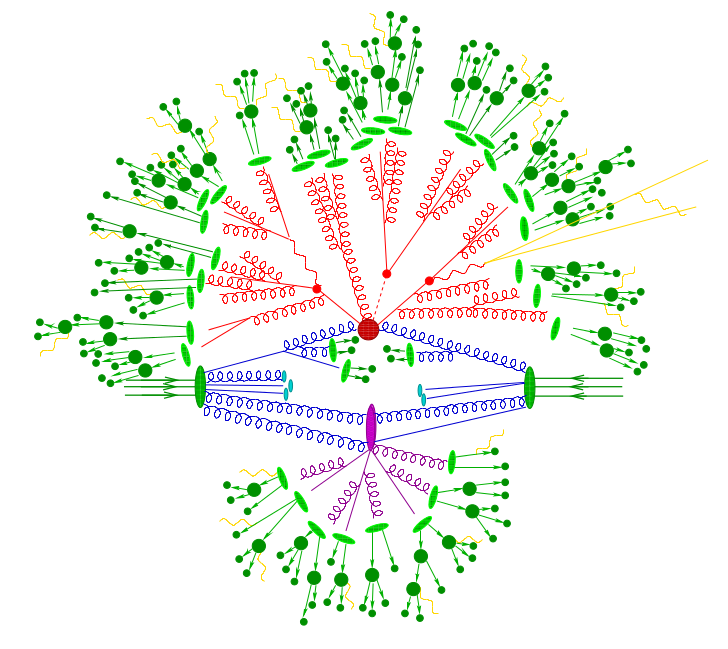
\includegraphics[scale=0.55]{Figures/HadronCollisionProcess.png}
\end{center}
\caption{Graphic visualisation of a hadron collision process where two partons come in from the right and the left, represented by the directional arrows. Two gluons (purple) form the hard scattering interaction (red circle). This section of the process depicts the matrix element calculation. In the hard scattering interaction prompt decays and parton showers then take place as represented by the smaller red circles. Finally, the hadronisation process begins (green circles). We also observe collinear gluon emissions as well as underlying event particles stemming from a softer collision with other partons in the hadrons. This is represented by the purple circle. \cite{HadronCollisionProcess}.}
\label{fig-HadronCollisionProcess}
\end{figure}

\section{Computing}

\subsection{Event Data Model}

Physically, an event is the result of the hard scattering process created when the LHC collides two bunches of protons together. We cannot know the full properties of an interaction without processing the data, and this is where the Event Data Model (EDM) is derived. The information about the event is measured as energy deposits, clusters, and tracks in each sub-detector of the CMS experiment that is read out by a series a processing electronics. When it comes to reconstructing the data and performing statistical analysis, we read in an event as a C++ object storing the raw data. These objects are presented to a user stored as ROOT files \cite{Brun199781}. There are three different data formats that data is stored as, each of which contains a different level of precision for describing events. The three levels are as described below.

\begin{description}
	\item[RAW] file formats contain very primal information about the data, including the L1 and HLT decisions. At this stage events have a size of roughly 1.5 MB. 
	\item[RECO] is the next step in the formatting of data by reconstructing events obtained from the RAW format with pattern recognition and compression algorithms. This includes reconstructed detector hits, calorimeter clusters, and reconstructed physics objects such as electrons, jets etc. The typical event size at this level is around 250 kB.
	\item[AOD] (Analysis Oriented Data) is created by filtering (performing quality checks etc) the RECO data from the reconstructed detector-level objects, where the higher level physics objects are calculated. The size of the events is reduced to $\sim50$ kB.	
\end{description}

Almost all physics analysis groups use the RECO and AOD data formats. All data used in this analysis uses the AOD data format, where event sizes are reduced by filtering the RECO data, as can be seen in Table \ref{tab-MCSamples}. The objects are delivered in the data files as C++ objects, which are then transformed into vectors or plain basic types. By selecting on the physics objects that are central to our analysis, we can further reduce the event size to $\sim$3 kB, which we call the ``skimming", thus reducing the run time of an analysis. The processing of RECO and AOD formats for analysis begins with taking the data and using a specifically designed framework to process a set of ``nTuples'' for each physics process, and categorising them into classes, such as objects. The benefit of constructing such ``nTuples'' lies in the reduction of processing time by allowing the analysis to be run locally, rather than re-processing the full dataset in AOD, RECO, or RAW from each time. 

\subsection{Analysis Software} \label{subsec-AnalysisSoftware}

Analysis is usually performed within a computing environment specific to an experiment. CMS provides an extensive software framework, CMSSW \cite{CMSSW}, that provides users with a large range of algorithms to create, handle, and analyse data. $\CMSSW$ is fundamental in regards to MC simulation, detector calibration and alignment, and then for the reconstruction of data and analysis thereof. The framework is a modular structure that combines a single configurable executable (cmsRun) with a number of plugin modules containing event processing algorithms. $\CMSSW$ is continuously being updated to keep up-to-date with new analysis techniques and processes. The versions of $\CMSSW$ used in this analysis are listed below:

\begin{itemize}
	\item CMSSW\_5\_3\_9 for the analysis of $t\bar{t}+\gamma$.
	\item CMSSW\_5\_2\_10\_nTuple for the ntuple processing for the $t\bar{t}+\gamma$ analysis.
\end{itemize} 

The framework used is of a modular design, similar to $\CMSSW$. The code is split into different modules designed to model the data at various stages of processing. We essentially design four modules to carry out the reading-in of the data, transferring it into a readable C++ format, selecting and implementing cuts on our events, and outputting the information in the form of a histogram in order to statistically analyse the data, as described below. 

\begin{itemize}
	\item Reader files that translate plain data types stored in ROOT files into C++ objects. 
	\item Reconstruction objects process the output of the readers in the form of real objects, such as leptons and quarks.
	\item Selections are written for each decay channel in an analysis to select on objects that exist in the final state of an event.
	\item Analysers are used to create histograms of different variables at various stages of selection, implement scale factors, and add weights to samples. 
\end{itemize}

\section{Simulation of the CMS detector}

The simulation of the CMS detector is an incredibly complex task and very time consuming to run such a simulation. In order to perform such a procedure $\GEANTfour$ \cite{GEANT4} is used to simulate the geometry of the whole detector, divided into sub-detectors, and track the particles as they pass through the different materials. Implemented within the $\CMSSW$ framework are two packages that perform detector simulation, Full Simulation (FullSim) \cite{FullSim} and Fast Simulation (FastSim, previously named FAMOS) \cite{1742-6596-513-2-022012}.  
In the FastSim package physical processes are described in detail, such as the electromagnetic and hadronic interactions, energy deposits, and electronic detector responses. The FastSim package is designed with a much lower level of detail incorporated and reduces the computational time by 3 orders of magnitude. This allows analysts to carry out custom MC productions within a reasonable time. A comparison between the two packages is shown in Figure \ref{fig-FullSim}. 

\begin{figure} 
\begin{center}
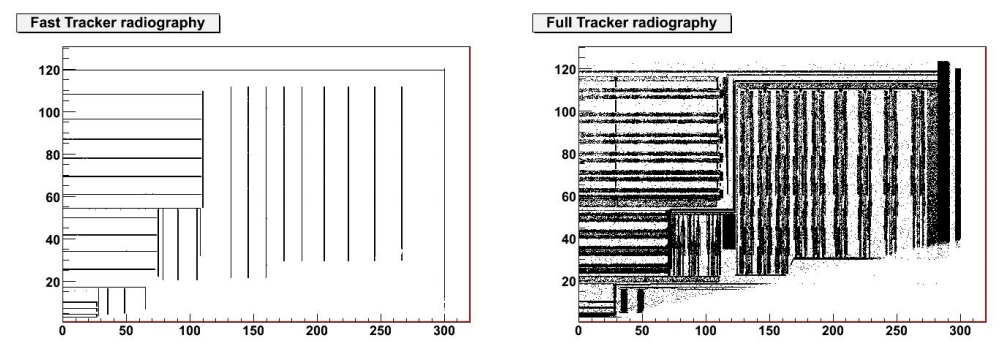
\includegraphics[width=\textwidth]{Figures/FullSim.png}
\end{center}
\caption{A radiography of a quarter of the simulated tracker geometry in the (a) fast and (b) full simulation \cite{1742-6596-513-2-022012}. The data points are from the vertices of converted photons, whereby we have a much larger of simulated events in the fastsim.}
\label{fig-FullSim}
\end{figure}

\section{Monte Carlo Simulation}

\subsection{Monte Carlo event generators} \label{subsec-MCEventGenerators}

MC generators are programs that simulate the properties of particles such that results can be compared to those obtained from data in order to perform a statistical analysis and verify findings. CMS uses many event generators in order to simulate specific physics processes that are of interest. Hard scattering processes are simulated via matrix element calculation and then parton showering is subsequently added. In order to convolute the two procedures a matching is implemented. Finally, hadronisation is then modelled as the showered partons form colourless bound states with other partons. MC event generators produce a list of all particles/partons that are created in an event along with their kinematic properties, such as p$_T$, and includes production of underlying events (UE) and additional primary vertex interactions from pile-up (PU). Underlying events are classified as any source of interaction produced that does not originate from the initial hard scattering process, such as initial and final state radiation (ISR and FSR), and remnants from the beam. We define PU as any other interaction produced from the same bunch crossing as our hard scattering. Bunch crossings can contain up to 20 different interactions, that is to say 20 different primary vertices are observed. Figure \ref{fig-HadronCollisionProcess} shows the hard scattering collision process as produced by MC event generators. 

In the analysis presented in this thesis each physical process was simulated by different MC event generators, such as $\WHIZARD$ $\MADGRAPH$ $\PYTHIA$ $\MCATNLO$ $\POWHEG$. The MC event generators which are used in this analysis, as previously mentioned, are described in more detail below. Generators are usually combined by interfacing with another generator in order to optimise for each simulation step described in Section \ref{sec-EventReconstruction}. An example of this can be seen within the main background sample for this analysis, the $t\bar{t}$ sample, which is generated using both $\MADGRAPH$ and $\PYTHIA$.   

\begin{description}

	\item[\WHIZARD] \cite{WHIZARD} is a LO event generator designed to calculate multi-particle scattering cross-sections efficiently and simulated event samples. Tree-level matrix elements are automatically generated for arbitrary partonic processes, in particular the MSSM is supported including an interface to the SUSY Les Houches Accord (LHA) input format. It is also possible to interface matrix elements from alternative processes, such as loop corrections. WHIZARD uses a multi-channel method for phase space integration, meaning that it involves simultaneous use of multiple phase space parametrisations corresponding to dominant Feynman diagrams, and is able to calculate numerically stable signal and background cross-sections and also generate unweighted event samples with a reasonable efficiency for final state events containing up to 6 or more particles, meaning that it generates uniformly distributed events each contributing the same event weight to the sample. The polarisation of initial and final states is treated in the same manner, and quark and lepton flavours are automatically summed over where needed. For hadron collider physics studies, the standard LHAPDF library is incorporated. For fragmentation and hadronisation of the final states, $\PYTHIA$ and $\HERWIG$ interfaces are provided, both of which follow the Les Houches Accord. 

	\item[\MADGRAPH] \cite{MADGRAPH5} is a leading order multi-purpose matrix-element MC generator. Similar to the WHIZARD generator, $\MADGRAPH$ automatically generates matrix elements for scattering processes with up to 6 and above final state particles. The matching of matrix elements to parton showers is performed following the MLM prescription \cite{Hoche:2006ph} only if a parton-jet pair satisfies a predefined $\Delta R$ requirement, and if none, or more than one jets, are found then the event is rejected. There is also a certain p$_T$ threshold for partons that they must pass in order to be considered for matching.

	\item[\PYTHIA] \cite{1126-6708-2006-05-026} is a widely used tool in the particle physics community. It is used for the generation of events within high-energy collisions, and it does so by utilising a complex set of physics models to process the evolution of a 2-body (or more) scattering to a complex multi-particle final state. The generator contains a library of hard processes, models for parton showers for initial and final states, matching among hard processes and parton showers, multi-parton interactions, beam remnants, string fragmentation and particle decays.  

	\item[\MCATNLO] \cite{1126-6708-2002-06-029} provides a method for matching next-to-leading order (NLO) calculations of QCD processes with a particle shower from simulation in MC. $\MCATNLO$ improves on many aspects with respect to a LO generator, such as $\PYTHIA$. Aspects such as the total exclusive rates are accurate to NLO, hard emissions are treated as in NLO computations with soft/collinear emissions handled by MC, and matching between hard and soft emission regions is smooth. This provides an advantage for heavy flavour physics, such as top quark production. A small amount of events with negative weights are generated, however the process of unweighting is possible with a reasonable efficiency. 

	\item[\POWHEG] \cite{1126-6708-2007-11-070} (Positive Weight Hardest Emission Generator) is a NLO event generator similar to $\MCATNLO$ described above. The difference between the two arises in the basic idea behind $\POWHEG$, whereby it generates the hardest radiation first before passing the event to any shower generator to perform subsequent, softer radiation. Thus, as it does not depend on any parton shower program in particular, the output of $\POWHEG$ can be easily interfaced with any shower generator capable of handling the given user process. Another feature of $\POWHEG$ is that events can be created with positive (constant) weight.  


\end{description}	

\section{Simulated samples for the $t\bar{t}+\gamma$ analysis}

As previously mentioned, different MC samples are simulated using different event generators for various physical processes. Table \ref{tab-MCSamples} provides all the different MC sample datasets used in the $t\bar{t}+\gamma$ analysis along with their respective cross-sections and number of processed events in each sample. This section will focus on background samples where generation of the signal $t\bar{t}+\gamma$ sample can be seen in Section \ref{sec-mcsim} It can be seen that the main background to this analysis, TTJets ($t\bar{t}$), is was generated using the $\MADGRAPH$5 event generator and interfaced with the $\TAUOLA$ generator. $\TAUOLA$ is a MC event generator designed specifically for the modelling of tau lepton decays. The samples are then passed to $\PYTHIA$6 for parton showering and hadronisation as described in Section \ref{subsec-MCEventGenerators}. Each $t\bar{t}$ decay process, fully-leptonic, semi-leptonic, and fully hadronic is treated individually and generated as three independent samples. The advantages of treating the decay modes separately are that no scale factor has to be implemented in order to account for the different branching ratios of each decay channel and it is also more convenient to observe the $t\bar{t}+\gamma$ content in each channel separately.

Similarly, both Drell-Yan samples, W+Jets, $W+\gamma$, $Z+\gamma$, and diboson background samples are also simulated in the same fashion as the TTJets samples. Single top events are simulated in a slightly different fashion, whereby they are generated by the $\POWHEG$ generator, also described in Section \ref{subsec-MCEventGenerators}. Again, the events are then passed to $\PYTHIA$6 to model parton showering and hadronisation. Single top samples are also split into different decay modes: tW, s-channel, t-channel. Top quarks and anti-top quark processes are treated separately and simulated in different samples.

\begin{sidewaystable} 
\begin{center}
\resizebox{\textwidth}{!}{ 

\begin{tabular}{|l| p{12.5cm} |c|p{2cm}|}
\hline
	\textbf{Process} & \textbf{Dataset} & \textbf{$\sigma$ (pb)} & \textbf{Number of events} \\
\hline
	$t\bar{t}+\gamma (2\to5)$ & /LHE2EDM\_WHIZARD\_2to5\_ttA/htholen-FULLSIM\_STEP2\_WHIZARD\_2to5\_ttA-da43ae45efb6a7c35e17aad82de2e2cd/USER & 1.8 & 1074860 \\
	$t\bar{t}+\gamma (2\to7)$ & /TTGamma\_TuneZ2star\_8TeV-madgraph-tauola/Summer12\_DR53X-PU\_RD1\_START53\_V7N-v1/AODSIM & 1.8 & 916500\\ 
\hline	
	$t\bar{t}(Leptonic)$ & /TTJets\_FullLeptMGDecays\_8TeV-madgraph/Summer12\_DR53X-PU\_S10\_START53\_V7A-v2/AODSIM & 245.8 & 12119013\\
	$t\bar{t}(Hadronic)$ & /TTJets\_HadronicMGDecays\_8TeV-madgraph/Summer12\_DR53X-PU\_S10\_START53\_V7A\_ext-v1/AODSIM & 245.8 & 31223821\\
	$t\bar{t}(Semileptonic)$ & /TTJets\_SemiLeptMGDecays\_8TeV-madgraph/Summer12\_DR53X-PU\_S10\_START53\_V7A\_ext-v1/AODSIM & 245.8 & 25424818\\
	$t\bar{t}(Inclusive)$ & /TTJets\_MassiveBinDECAY\_TuneZ2star\_8TeV-madgraph-tauola/Summer12\_DR53X-PU\_S10\_START53\_V7C-v1/AODSIM & 245.8 & 6923652\\
\hline	
	Drell-Yann, $10 < m\_{ll} < 50$ & /DYJetsToLL\_M-10To50\_TuneZ2Star\_8TeV-madgraph/Summer12\_DR53X-PU\_S10\_START53\_V7A-v1/AODSIM & 11050.0 & 37835275\\
	Drell-Yann, $m\_{ll} > 50$ & /DYJetsToLL\_M-50\_TuneZ2Star\_8TeV-madgraph-tarball/Summer12\_DR53X-PU\_S10\_START53\_V7A-v1/AODSIM & 3350.0 & 30459503\\
\hline	
	$Z+\gamma$ & /ZGToLLG\_8TeV-madgraph/Summer12\_DR53X-PU\_RD1\_START53\_V7N-v1/AODSIM & 159.12 & 6588161 \\
\hline	
	Single Top tW & /T\_tW-channel-DR\_TuneZ2star\_8TeV-powheg-tauola/Summer12\_DR53X-PU\_S10\_START53\_V7A-v1/AODSIM & 11.1 & 497658 \\
	Single TopBar tW $\bar{t}$ & /Tbar\_tW-channel-DR\_TuneZ2star\_8TeV-powheg-tauola/Summer12\_DR53X-PU\_S10\_START53\_V7A-v1/AODSIM & 11.1 & 493460 \\
	Single Top t & /T\_t-channel\_TuneZ2star\_8TeV-powheg-tauola/Summer12\_DR53X-PU\_S10\_START53\_V7A-v3/AODSIM & 56.4 & 99876 \\
	Single TopBar t & /Tbar\_t-channel\_TuneZ2star\_8TeV-powheg-tauola/Summer12\_DR53X-PU\_S10\_START53\_V7A-v1/AODSIM & 30.7 & 1935072 \\
	Single Top s & /T\_s-channel\_TuneZ2star\_8TeV-powheg-tauola/Summer12\_DR53X-PU\_S10\_START53\_V7A-v1/AODSIM & 3.79 & 259961 \\
	Single TopBar s & /Tbar\_s-channel\_TuneZ2star\_8TeV-powheg-tauola/Summer12\_DR53X-PU\_S10\_START53\_V7A-v1/AODSIM  & 1.76 & 139974 \\
\hline	
	W+Jets & /WJetsToLNu\_TuneZ2Star\_8TeV-madgraph-tarball/Summer12\_DR53X-PU\_S10\_START53\_V7A-v2/AODSIM & 36257.2 & 57709905 \\
\hline	
	$W+\gamma$ & /WGToLNuG\_TuneZ2star\_8TeV-madgraph-tauola/Summer12\_DR53X-PU\_S10\_START53\_V7A-v1/AODSIM & 553.92 & 4802358 \\
\hline	
	Diboson WW & /WW\_TuneZ2star\_8TeV\_pythia6\_tauola/Summer12\_DR53X-PU\_S10\_START53\_V7A-v1/AODSIM & 56.0 & 10000431\\
	Diboson WZ & /WZ\_TuneZ2star\_8TeV\_pythia6\_tauola/Summer12\_DR53X-PU\_S10\_START53\_V7A-v1/AODSIM & 33.6 & 10000283\\
	Diboson ZZ & /ZZ\_TuneZ2star\_8TeV\_pythia6\_tauola/Summer12\_DR53X-PU\_S10\_START53\_V7A-v1/AODSIM & 8.2 & 9799908\\
\hline	
\end{tabular}
}
\end{center}
\caption{Dataset information for signal and background MC samples.}
\label{tab-MCSamples}
\end{sidewaystable}


\section{Simulation of the $t\bar{t}+\gamma$ Signal Sample} \label{sec-mcsim}

Three different techniques were used to define the $t\bar{t}+\gamma$ signal process. The concepts are illustrated in Figure \ref{fig-MatrixElementCalculation} and shows the final state of the process using each technique \cite{heinerthesis}. The parton distribution function CTEQ6L1 \cite{Pumplin:2002vw} is interfaced to $\WHIZARD$ via LHAPDF \cite{Whalley:2005nh}. The process utilises variable renormalisation and factorisation scales. This is such that, event by event, the two are set to $172.5 \GeV$ (m$_t$) plus the E$_T$ of the generated photon. Upon varying the scale of each, we arrive at a systematic uncertainty of $^{+7.0}_{-8.3}\%$, as shown in Chapter \ref{chap-SystematicUncertainties}. Initial and final state radiation is taken into account, as well as hadronisation, and is simulated using \PYTHIA6 \cite{Sjostrand:2006za}, $\TAUOLA$ and $\PHOTOS$ \cite{Was:2006my} as preconfigured in CMSSW. We use the same configuration as for the top-pair sample.

Restrictions on the final state particles have been set, named generation cuts, such that a proper integral is retained when calculating matrix elements. As a method to cope with infra-red divergences, soft gluon emissions, a minimum energy or momentum is required. We treat collinear divergences (collinear parton splitting) by introducing a minimum distance in the $\eta - \phi$ plane. These cuts likely will not affect the measurement due to the cuts within selection being tighter than generator levels cuts. The different generation cuts are described in brief below:

\begin{description}
\item[2 $\to$ 3] At this level only quantum mechanical interferences from initial state radiation are considered. The CPU time required in for tree level processes is moderate.

\item[2 $\to$ 5] In this case, the decay of the top quark is included and thus photons that have radiated from a W boson or a b-quark, as well as interference effects between the two, must be taken into account. This is a significant process, as we must expect photons stemming from a W or b to contribute significantly to our signal. Photons that are radiated from the W are considered negligible, because the W decay products are highly boosted in top-quark events giving rise to, mostly, collinear emissions. 

\item[2 $\to$ 7] In this scenario we consider photon radiation and interference from all decay products. CPU time is much more intensive in this case due to the many more Feynman diagrams to be computed.                                                                            

\begin{figure} 
\begin{center}
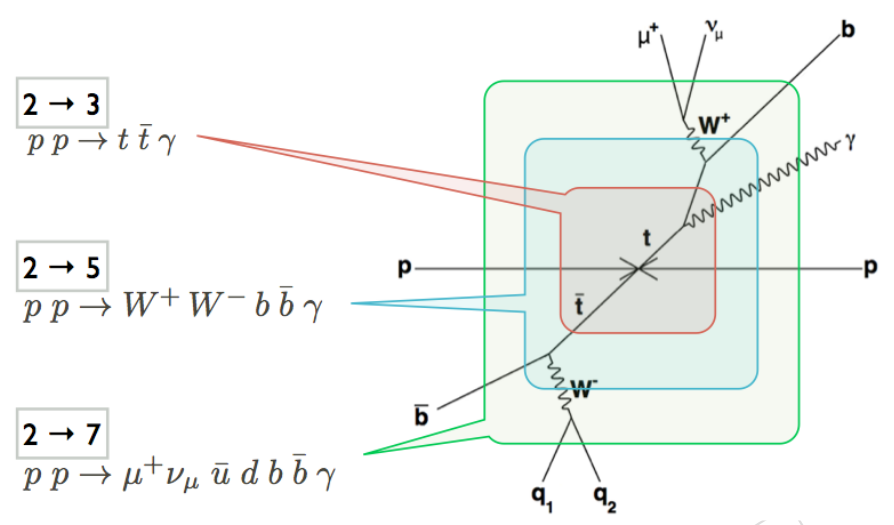
\includegraphics[width=\textwidth]{Figures/MatrixElementCalculation.png}
\end{center}
\caption{Process generation. The red, blue, and green boxes depict the matrix element calculation. Background processes with the same final state are included as well \cite{heinerthesis}.}
\label{fig-MatrixElementCalculation}
\end{figure}
                               

\end{description}

Originally, this analysis used the $2 \to 5$ technique with initial generator level cuts of $E_T > 20$ GeV and $\Delta R(\gamma, b/\bar{b}) > 0.1$ using WHIZARD \cite{WHIZARD}, which is a leading order (LO) event generator. The variable factorisation and renormalisation scales are set to $m_{top} + E_T(\gamma)$, and a scale variation uncertainty of 8\% has been applied to the WHIZARD $t\bar{t}+\gamma$ cross-section result, which gives $1.8 \pm 0.5$ pb as the SM expectation for the signal process, where the scale variation uncertainty, and uncertainty on the k-factor (the ratio between the NLO and LO cross sections as a function of some observable) are added in quadrature. 


\subsection{Official $t\bar{t}+\gamma$ $2 \to 7$ sample production}

The final version of the analysis uses the factorised $2 \to 7$ process for the simulation of the $t\bar{t}+\gamma$ signal sample. Instead of computing one single matrix element for the complete $t\bar{t}+\gamma$ process, we factorise the process into individual processes and calculate the matrix element for each sub-process. The major restriction on the calculation of the matrix element lies in the computational time, such that using a factorised matrix element method vastly reduces the computation time to calculate the matrix element. The matrix element is divided in the following manner:

\begin{align}
pp \to t\bar{t}+\gamma, \quad t \to bxx', \quad \bar{t} \to \bar{b}xx' \\
pp \to t\bar{t}, \quad t \to bxx'\gamma, \quad \bar{t} \to \bar{b}xx' \\
pp \to t\bar{t}, \quad t \to bxx', \quad \bar{t} \to \bar{b}xx'\gamma 
\end{align}

where $x = u,d,s,c,\bar{u},\bar{d},\bar{s},\bar{c}, e^{\pm}, \mu^{\pm}, \tau^{\pm}, \nu_{e,\mu,\tau}, \bar{\nu}_{e,\mu,\tau}$.

In order to verify the factorisation method, we generated a sample using WHIZARD with the full, un-factorised, $2 \to 7$ matrix element generation process, which we then compared to a sample simulated in WHIZARD using the factorised matrix element method. The results of this comparison can be seen in Figure \ref{fig-WHIZARDfullvsfactorised}, where we see a good agreement in the shapes of observables. We observe small fluctuations between bins within the full $2 \to 7$ sample, which we attribute to the number of events. We can therefore verify that the method can be used as a good approximation of the full $2 \to 7$ process.

Upon validation of the factorisation method for the full process, we observe the method to be a good compromise between accuracy and computational time. A comparison is then conducted between the $\MADGRAPH$ and WHIZARD event generators using the full $2 \to 7$ process. Within the WHIZARD framework, we are unable to compute the three factorised processes at the same time, and must therefore generate the individual processes separately and later combine them, whereby scaling is taken into account. 

For both generators, the original $pp \to t\bar{t}+\gamma$ process and the decay of the top quarks are distinct processes. The $\MADGRAPH$ framework handles both processes internally, however we must simulate the two must be handled individually in the WHIZARD framework and an extra set of kinematic cuts must be implemented, as shown below.

\begin{itemize}
	\item $p_T(\gamma) > 1$ GeV
	\item $\Delta R (\gamma, X) > 0.1$
\end{itemize}

These cuts are required to be softer than the final generator cuts, due to the dilution of kinematics by resolution effects at the value of the cuts. This is such that if the value of cuts used for decays is too close to the final generator cuts, resolution effects may be modelled incorrectly. When calculating the cross-section, WHIZARD does not take the final generator cuts into consideration. They are simply used to select events which are then written to the output file. The cross-section must be re-weighted when taking individual efficiencies into account, leading to the simulation taking more time than it would with the final generator cuts included, where a vast amount of generated events are rejected by the tighter cuts.

It must be noted that for simplicity, in the comparison we only select semi-leptonic events in the muon channel. However, for the full sample we incorporate all decay channels for the $2 \to 7$ process in order to be inclusive as possible since the sample will be an official CMS sample. 

\begin{figure} 
\begin{center}
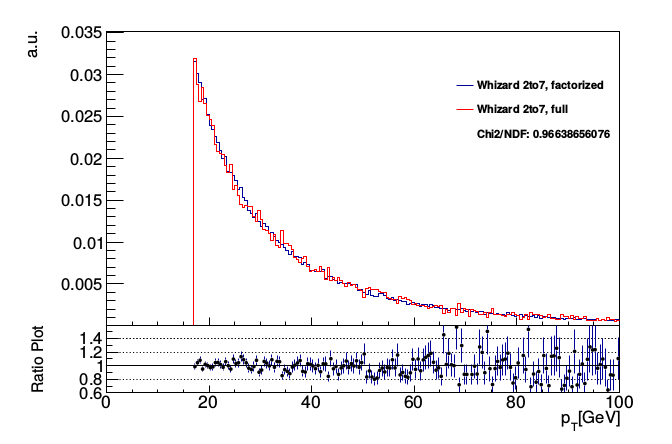
\includegraphics[width=0.9\textwidth]{Figures/WHIZARDfullvsfactorisedPT.png} \\
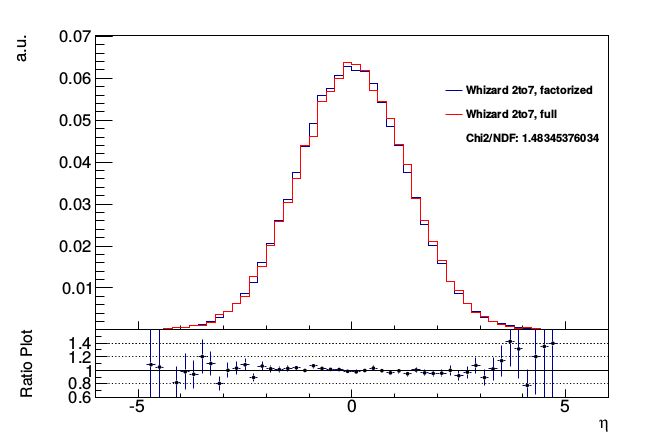
\includegraphics[width=0.9\textwidth]{Figures/WHIZARDfullvsfactorisedEta.png} \\
\end{center}
\caption{Comparison between the full and the factorised $2 \to 7$ process using samples generated with WHIZARD. All distributions are normalised to unity. \cite{ttgammasimulation}}
\label{fig-WHIZARDfullvsfactorised}
\end{figure}  

We calculate the cross-sections to be 

\begin{equation}
\WHIZARD : \sigma_{t\bar{t}+\gamma} = 1408 \xspace \text{fb}, \quad \MADGRAPH : \sigma_{t\bar{t}+\gamma} = 1227.1 \pm 0.4 \xspace \text{fb}
\end{equation}

for each event generator, respectively. We note that there is no associated error with the WHIZARD cross-section, this is due to the cross-section calculated with this event generator not taking the final cuts on the decay products into account. The final cross-section is calculated from the remaining number of events. Additionally, the branching ratios for the top decays are not included within the cross-section calculation, as additional calculations are required by the user. This is more of a feature in channels where a photon is required. 

The calculation steps, described previously, are estimated individually and the uncertainty on each usually contributes to the overall uncertainty by propagating them onto the final value. However, this is not calculated in this analysis, because the cross-sections are used to compare the event generators. Thus, an exact calculation of the errors is not necessary, and a NLO cross-section is used in the analysis which renders the differences inconsequential. The difference of 12.9\% observed between the two generators is thus within the expected range of deviation. 

A comparison between the two event generators for the factorised $2 \to 7$ process, for three key variables, can be seen in Figure \ref{fig-WHIZARDvsMADGRAPH}. We observe a good agreement between the two event generators except for small discrepancies in the angle between the photon and b quark at low values of $\Delta R (\gamma, b)$. We regard this discrepancy as irrelevant to our analysis due to the manner in which jets and isolation is handled in a proton-proton collider experiment such as CMS. Another explanation could lie within the normalisation process of the WHIZARD sample, and could affect the shapes of the distributions.

\begin{figure} 
\begin{center}
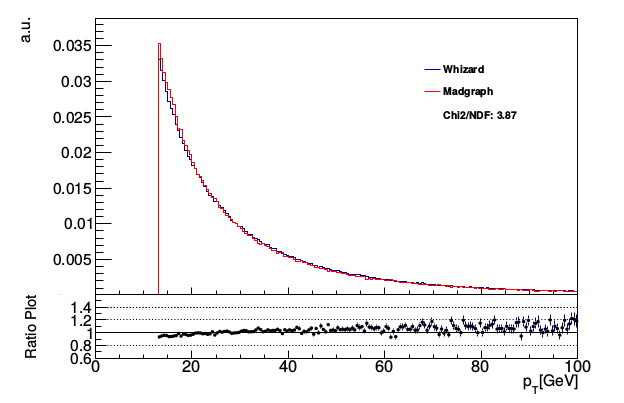
\includegraphics[width=0.8\textwidth]{Figures/WHIZARDvsMADGRAPHPT.png} \\
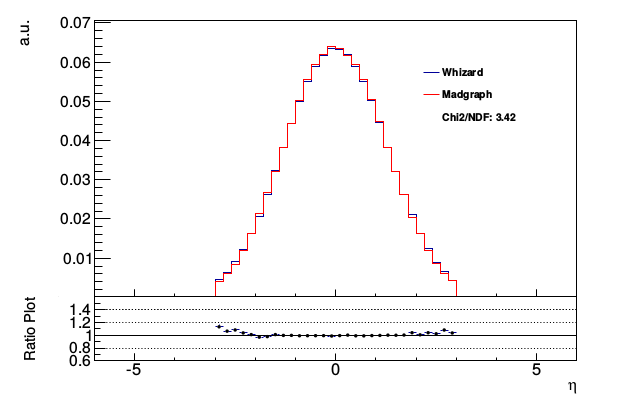
\includegraphics[width=0.8\textwidth]{Figures/WHIZARDvsMADGRAPHEta.png} \\
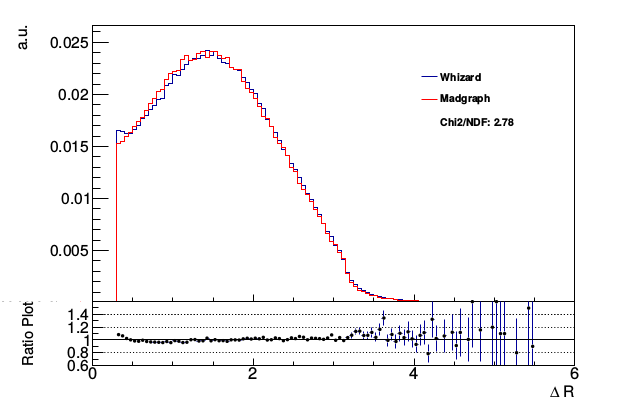
\includegraphics[width=0.8\textwidth]{Figures/WHIZARDvsMADGRAPHDR.png} \\
\end{center}
\caption{Comparison between the $\MADGRAPH$ and WHIZARD generators for the factorized $2 \to 7$ process. All distributions are normalized to unity. \cite{ttgammasimulation}}
\label{fig-WHIZARDvsMADGRAPH}
\end{figure}  

The cuts used in the generation of the \MADGRAPH MC sample are as shown below.

\begin{itemize}
	\item $p_T (\gamma) > 13 \GeV$
	\item $|\eta(\gamma)| < 3.0$
	\item $\Delta R (\gamma, all) > 0.3$, where ``all" refers to any other generator level particle
	\item $p_T (jet) > 15 \GeV$
	\item $p_T (b) > 20 \GeV$
	\item $|\eta (b)| < 5.0$
	\item $|\eta (jet)| < 5.0$
	\item $| \eta (lepton)| < 3.0$
	\item $\Delta R (jet, jet) > 0.5$
	\item $\Delta R (jet, lepton) > 0.5$
\end{itemize}

There is no cut on lepton transverse momentum, but there are cuts on the momenta of quarks (jets). This makes the ratio of hadronic and leptonic W decays generated with these cuts differ from W branching ratio without any cuts.

\section{Physics Object Reconstruction} \label{sec-ParticleObjectReconstruction}

The CMS experiment employs a complex algorithmic technique, Particle Flow (PF) \cite{CMS-PAS-PFT-09-001}, as part of a chain of reconstruction tools to reconstruct the full topology of events produced by collisions using information from each sub-detector. PF uses the information obtained from lower-level object reconstruction including tracking and clustering of energy deposits within each sub-detector. The primary goal of PF is to determine the object type, momentum, and energy for all objects within a singular event. Such objects include electrons, muons,  charged hadrons, neutral hadrons, and photons. This information is then used to reconstruct higher-level objects, such as jets and MET.

\subsection{Charged Particle Tracking} \label{subsec-ChargedParticleTracking}

The tracking of charged particles begins with the reconstruction of tracks in the inner detector system. As the charged particles traverse the detector they deposit energy which we call hits, an iterative tracking algorithm then inputs the information from a number of hits in order to reconstruct tracks of individual particles \cite{1748-0221-9-10-P10009}. By reconstructing the particle tracks we have access to information about the particle, such as the momentum before any effects from the magnet, and the impact parameter (IP), the distance of closest approach to this point used in later reconstruction. 

Around two thirds of the particles than constitute a jet are charged particles, therefore if we are able to accurately reconstruct the tracks of charged particles in the detector, and the accuracy for correctly reconstructing a jet increases greatly. As all objects are reconstructed using the PF algorithm, which uses tracker information to fit tracks before reconstructing higher-level objects (Section \ref{sec-HigherLevelObjects}) we see that information gleaned from tracker hits are vital for physics analysis. Several properties of tracks from the inner detector system contribute to its importance in reconstructing tracks, such as the $p_T$ resolution which, for charged hadrons with a $p_T$ of $\mathcal{O}(10^2) \GeV$, is significantly better than in the calorimeter systems.

One of the key parameters in object reconstruction is the track efficiency, the number of real tracks found over the number that incorrectly reconstructed or originate from a different source (`fake tracks'). Therefore, a high tracking efficiency is required in order to use the PF algorithm to it's full potential, and thus an iterative algorithm for tracking was designed \cite{1748-0221-9-10-P10009}. The tracking algorithm can be broken down into roughly 5 processes, which are described below:

\begin{description}
	\item[Local Reconstruction] records signals in the silicon strips and pixels, converts them into `digis' and then groups them into 
	clusters. Both the position and uncertainty associated with an individual digi is calculated during this stage of reconstruction.
	\item[Track Seeding] defines seeds, the basis of full particle reconstruction, by combining into `pairs' and `triplets' hits from the pixel 
	detector of the inner tracker.
	\item[Pattern Recognition] combines hits from the tracker and combines them in order to reconstruct potential particle trajectories, by 
	starting at the centre of the tracker system and working outwards through each layer. The tracks are then filtered using a Combined Kalman 
	Filter \cite{Billoir1989390}, which is a combinatorial variation on a Global Kalman Filter. All hits are taken into account from a single 
	layer of the tracker and used as input information for a `proto-track', which is then used to calculate an estimate of the position and the 
	uncertainty of the position in the next layer of the tracker. It is important that we must also take into account the energy loss as the 
	particle traverses each layer of the detector. If we find several hits that are considered as signal, then we define multiple tracks. We 
	must also include the case where a particle is highly energetic, such that it only leaves deposits within some of the tracker layers and 
	not all.
	\item[Fitting] The Kalman filter then fits each of the reconstructed hits twice from the different layers defined in the pattern 
	recognition process. The first fitting process is performed using hits from central layers outwards, whereas the second fitting uses hits 
	from the outer layers inwards. The two fits are complimentary to one another and remove any bias obtained during the track clustering stage.
	\item[Quality Checking] removes tracks that are categorised as low quality, such that reconstructed hits have low hit multiplicity and a 
	high $\chi^2$. Low quality tracks arise from aspects such as inconsistencies and misreconstructed hits in the track finding process; a 
	single seed in the tracker layer can rise to multiple tracks, as well as multiple seeds originating from the same track, can be removed by 
	performing the quality check of tracks. 
\end{description}
 
The algorithm iterates over the process 6 times in order to filter out as many fakes/misreconstructed tracks as possible. For each iteration in 
the algorithm, cuts are loosened, such as the $p_T$, so that the tracking efficiency ($\epsilon$) is increased while minimising the number of 
fakes. At the end of each iteration, after passing the track quality testing, high quality tracks are removed and the iterative process 
restarts. For the first four iterations only the seeds from the pixel detector are incorporated into the algorithm, where the last two use 
information of hits from the silicon strip detector. By performing track reconstruction in this manner we include tracks that decay outside the 
pixel volume, such as long-lived particles, heavy flavour hadrons and $\tau$ leptons, and photon conversions. At the end of the 
process, we are able to reconstruct tracks for particles with at least 3 hits in the tracking system with a $p_T$ as low as 150 GeV, a primary 
vertex originating at least 50 cm from the beam axis, and all with a fake-rate of approximately $1\%$ \cite{1748-0221-9-10-P10009}. 

\subsection{Primary Vertex Reconstruction} \label{subsec-PrimaryVertexReconstruction}

Our ability to identify and reconstruct vertices of particles in events has a large impact on the reconstruction of whole event topologies and kinematics. If we are to correctly assign tracks to collisions, we must efficiently reconstruct the coordinates of the primary vertex. The same can also be said for secondary vertex reconstruction, used for the identification of heavy-flavour hadrons and $\tau$ leptons, as well as photon conversions. The main challenges encountered in vertex reconstruction stem from multiple overlapping events from a high track density and particle interactions within the tracker volume. 

Once we have reconstructed all charged particle tracks to a sufficient degree of efficiency, we begin use this information to reconstruct the primary vertices (PV) for interactions within an event. Similar to the reconstruction of particle tracks, tracks must pass a selection criteria in order to be defined as originating from a primary vertex. A primary vertex must be defined as having a small impact parameter with respect to the beam line, a minimum number of hits in each layer of the pixel and silicon strips, and a small $\chi^2$ significance ($\chi^2/N_{d.o.f}$). For the tracks that meet the imposed requirements, they are then clustered along the z-axis at their point of closest approach to the beam. We then define these as our primary vertex candidates and begin the fitting process.

An Adaptive Vertex Fitter (AVF) \cite{1742-6596-110-9-092009} is then implemented and uses a 3D fit, reconstructing the tracks using (x,y,z)-values such that the track is three-dimensional, to reconstruct the PV candidates, whereby each track is assigned a weight that is a function of its $\chi^2$ contribution to the vertex. After each iteration of the fitting process, the given weights are translated to the new vertex position. 

In order to discern the primary vertex from the hard-scattering event that we are interested in, vertices are listed in descending order of $p_T$. As we expect events from pile-up to have a lower sum of $p_T$ to the hard process, we take the primary vertex with the highest $p_T$ and assume the rest are from pile-up.  

\subsection{Calorimeter Clustering Algorithm} \label{subsec-CalorimeterClusteringAlgorithm}

The granularity of the CMS HCAL is 25 times coarser than ECAL in order to separate spatially charged and neutral hadrons in jets with a transverse momentum above $100 \GeVc$. Therefore, we must employ a different algorithm for the identification and reconstruction of tracks within the different calorimeter systems. The calorimeter clustering algorithm is implemented to perform this task \cite{CMS-PAS-PFT-09-001}. The calorimeter clustering algorithm works independently of the PF algorithm, however energy deposits from charged hadrons are matched using the PF algorithm in order to provide a more accurate measurement of the energy. The two algorithms working in tandem are able to resolve high-$p_T$ and collinear tracks and thus reconstruct energy deposits from neutral hadrons and photons. Clusters of energy are formed by taking information from energy deposits within each calorimeter system, excluding the forward HCAL where each cell is large enough that it is considered a cluster.

%%%% More 

\subsection{The Particle Flow event reconstruction algorithm} \label{subsec-PFAlgorithm}

The particle flow (PF) algorithm \cite{CMS-PAS-PFT-09-001} uses information from each sub-detector to reconstruct and identify all stable particles produced in proton-proton collisions at the LHC, such as electrons, muons, photons, charged hadrons, and neutral hadrons, and determine their direction, energy, and type. The information is then used in a similar manner to events from MC generators in order to reconstruct higher-order objects, such as jets (from which we infer the directions and energies of the quarks and gluons), missing transverse energy (giving a rough measurement of the direction and energy of invisible particles, such as neutrinos), and tau leptons, and to tag b-jets.  

The design of the CMS detector is ideal for this type of reconstruction, due to it being completely hermetic around the interaction point with a 3.8 T magnetic field, thus the reconstruction of charged particle tracks (which make up around 2/3 of the total objects) is extremely efficient with a small fake-rate down to a low $p_T$ of around $150 \MeVc$ and pseudorapidities as large as $|\eta| < 2.6$. Energy deposits are recorded as `blocks' in the detector, which are then interpreted as particles within a particular sub-detector. The PF algorithm feeds the information obtained by each sub-detector into the `link' step, where it then groups together combinations of blocks that are likely to originate from particles. The combinations are then categorised as individual objects and stores a list of particles of each type. 

Particles are composed of several particle-flow elements from a number of CMS sub-detectors: one charged particle track, and/or various clusters in the calorimeters, and/or one muon track in the muon system. The link algorithm is then used to connect the tracks and energy clusters to reconstruct the particle, whilst removing possible double counting from any of the sub-detectors. Pairs of elements are found and `linked', such that the link is extrapolated to the end of a shower for a typical electron in the ECAL or the typical interaction length
of a hadron shower in the HCAL, where a distance parameter defines the quality of a `link'. Blocks of elements in each sub-detector are produced by the algorithm which are classes as directly or indirectly linked. The PF reconstruction process is made easier by its high granularity, such that each block contains a maximum of three elements, and thus the performance of the algorithm is independent of the event complexity. However, the size of a block may be increased by up to a cell to account for the non-uniformity of the calorimetry system. 

Once blocks are processed by the link algorithm, they are then passed to the PF algorithm, where the objects are reconstructed and identified on an event-by-event basis. When an object is fully reconstructed, the tracks and clusters from the block are then removed from the collection and the next object is reconstructed. The first object type to be reconstructed is the muon, due to the efficiency of identifying muons. We measure muons from their associated Global and Tracker tracks, such that if they are within 3 standard deviations from each other we call the object a PF muon. The tracks and clusters associated with the blocks are then removed from the collection. 

Secondly, electrons are identified and reconstructed from the, now much smaller, collection of tracks. The GSF method of associating clusters (described in Section \ref{subsec-ElectronReconstruction}) is used to differentiate between charged hadrons and electrons, and the electromagnetic shower must be narrow in $\eta$. Charged pions give rise to a source of fake electrons and are vetoed by other such parameters as the number hits and $\chi^2$. Many other variables are then input into a multivariate analysis (MVA) tool which then provides a discriminant on whether or not the particle is an electron. If the particle passes the MVA (Table \ref{tab-ElectronMVAID}) it is then labelled as a particle flow electron.

By process of elimination, all that remains are charged hadron, neutral hadron, and photon candidates. By matching any charged tracks with an associated HCAL cluster, we can define these particles as PF charged hadrons. By implementing a distance parameter we make sure not to double count. We are then able to remove tracks associated with charged hadrons. Any remaining energy deposits in the HCAL is then known to originate from photons or neutral hadrons, differentiating between the two by the shower shape of the candidate. One can differentiate by using the energy profiles of electromagnetic showers, which are well predicted by Monte Carlo. We can thus define PF neutral hadrons and PF photons. 

\begin{figure}
\begin{center}
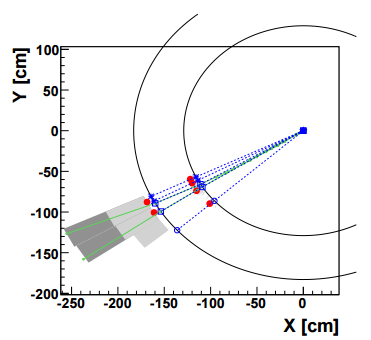
\includegraphics[width=0.6\textwidth]{Figures/PF.png}
\end{center}
\caption{The (x, y) view \cite{CMS-PAS-PFT-09-001}.}
\end{figure}

\begin{figure}
\begin{center}
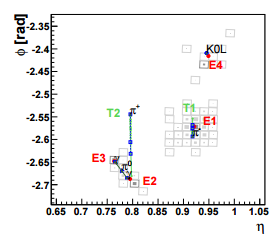
\includegraphics[width=0.7\textwidth]{Figures/PFECAL.png} \\
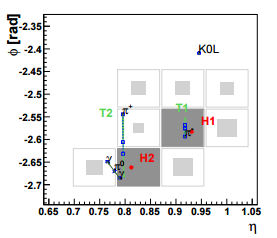
\includegraphics[width=0.7\textwidth]{Figures/PFHCAL.png} \\
\end{center}
%\caption{The ($\eta$, $\phi$) view on ECAL \cite{CMS-PAS-PFT-09-001}. 
\caption{The ($\eta$, $\phi$) view on HCAL \cite{CMS-PAS-PFT-09-001}.}
\end{figure}
   

\subsection{Electron reconstruction} \label{subsec-ElectronReconstruction}

For the $t\bar{t}+\gamma$ analysis it is imperative that the identification and energy-momentum requirements are measured extremely accurately as final state electrons, which are required in two of the three decay modes in the dilepton channel, can imitate a photon by passing the same selection, and therefore contaminating signal events. In order for electrons to be reconstructed with these strict requirements they are processed in a specific way.

The CMS ECAL and tracker systems are extremely accurate detectors, however reconstruction of energy deposits within the ECAL is still a complex task due to the density of material. As a charged particle traverses the detector volume, the energy lost due to interaction with the material is not negligible. Most charged particles are heavy enough such that the energy lost manifests in the form of multiple Coulomb scattering as the particle passes between material. However, in the case of electrons, the dominant process by which the energy is lost is due to Bremsstrahlung, the process by which photons are emitted upon passing through the electric and magnetic fields of a nucleus, such as the material in the detectors. 

Kalman fitters are a key tool used for the fitting of tracks in CMS due to their ability to incorporate noise amongst other inconsistencies,such as multiple scattering in track fitting, as Gaussian fluctuations. However, Bremsstrahlung radiation is non-Gaussian, and as a result electron tracks are poorly reconstructed with the standard Kalman filter fitting. To account for this, CMS provides a dedicated tool for the reconstruction of electrons using a Gaussian-sum filter (GSF) \cite{0954-3899-31-9-N01}. This method is implemented by calculating the trajectory of electrons using a `relaxed' Kalman filter, then re-fitted using a Gaussian-Sum Filter. The GSF method differs from the standard Kalman fitting method by computing uncertainties as the sum of multiple Gaussians rather than individual Gaussians. The downside to this method lies in the additional CPU time needed to process the events. 

The PF algorithm uses two different techniques of electron identification that are used as seeds when reconstructing electron \cite{CMS-PAS-PFT-10-003}. The first makes use of ECAL superclusters, extended clustering in $\phi$ due to Bremsstrahlung and photon conversions in the ECAL, as seeds and projects back from the centre of the supercluster to the innermost layer of the pixel detector, and is thus known as `ECAL-seeding'. It makes use of ECAL track properties, such as a narrow width in $\eta$ and a wide spread in the azimuthal angle, $\phi$. The energy deposits of the object and its associated Bremsstrahlung form a single supercluster, where the performance of this method lies the ability to correctly identify this. The method performs much more accurately in the high p$_T$ region of the electrons, such that there are much fewer potential track seeds and energy clusters in the ECAL are less likely to overlap with deposits from other objects, such as jets. This is especially true if the electron is part of a jet structure, and thus not isolated. Moreover, a high track multiplicity can complicate the backwards propagation from a supercluster and mimic the signal of another object.

The second, tracker-driven, method is much more suited for the efficient reconstruction of non-isolated and low p$_T$ electrons as they will most likely emit negligible amounts of Bremsstrahlung, and thus be fully reconstructed by extrapolating the tracks to superclusters. The cluster energy is then measured along with the track momentum, and if the ratio $E/p$ is close enough to unity then the track is selected. However, Bremsstrahlung is not always negligible and other track properties are used in the calculation. For example, the number of hits recorded in the inner tracker and the $\chi^2_{KF}$ of the Kalman filter fit are taken into account before refitting using a GSF, before being characterised by a multivariate estimation tool \cite{Roe2005577}. 

After both procedures have been performed the two collections of electron candidates are merged into one where a GSF is run in order to determine the final properties of the object. It is important for the GSF to be run at this stage in the process such that more hits can be included in the reconstruction, thus providing a more accurate description of the electron's energy and momentum lost by interacting with the detector material. Upon completion of the process, the GSF electrons are passed to the PF algorithm.

\subsection{Electron identification} \label{subsec-ElectronIdentification}

Electrons are identified in the ECAL and can be recognised by their distinct shower shape deposited within the calorimeter crystals. However, other objects such as charged hadrons, jets, and converted photons can have a very similar signature to an electron deposit and may be wrongly reconstructed as such. Therefore, in order to correctly reconstruct an electron candidate, we must implement further selection criteria. 

Individual physics analyses in CMS require different identification requirements tailored to personal needs, thus identification working points are initially required to be much looser than final cuts while still retaining a high efficiency of detecting electrons. When a further tight working point is implemented the efficiency for correctly selecting an electron increases. CMS uses various identification algorithms in order to correctly identify electrons: Simple cut-based ID, cuts in categories ID, particle flow ID, and MVA ID. Each of which are used in the analysis described in this thesis, and are described below.  

\begin{description}
	\item[Simple cut-based ID] Cut-based identification techniques, while not providing the greatest performance compared with other techniques, can be a useful tool in the understanding of the data and for making comparisons with MC.  Fewer variables from Table \ref{tab-ElectronMVAID} are used with this method, such as $H/E$, $\Delta \eta_{in}$ and $\Delta \phi_{in}$ between supercluster position and track direction at the vertex extrapolated to ECAL assuming no radiation, $\sigma_{i \eta i \eta}$ cluster and shape variables. \cite{CutBasedEleID}
	\item[Cuts in categories ID] is a more complex version of the simple cut-based identification techniques. It makes use of electrons originating from different sources, such as $Z$ and $W$ decays, while reducing the likelihood of wrongly selecting ``fake" electrons originating from photon conversions or jet mis-identifications, however the method has also been used to select electrons from alternative sources, such as the $J/\psi$. The problem of identifying electrons in CMS differs to that of other experiments due to the detector topology --- the large amount of material from the tracker directly in front of the ECAL and the high magnetic field make it difficult to efficiently reconstruct electrons. It has been found that many of the problems faced in the identification of electrons can be overcome by dividing the problem into categories. The most basic category sees the ECAL split into barrel and endcap regions due to the differences in topology in the two regions for both the inner tracker and ECAL. The second comes from the large amount of bremsstrahlung radiation in the tracker material, then using the measurement for $E/p$ to account for the poor reconstruction of the track. The final category divides electrons into high- and low-E$_T$ groups to correct for effects from the high magnetic field at high E$_T$.

	The cuts in categories method uses the same variables as the simple cut-based method with the addition of track conversion rejection (number of missing hits near beginning of track), and track isolations with tracker isolation ($\Delta R = 0.3$), ECAL Isolation (jurassic $\Delta R = 0.4$), HCAL Isolation ($\Delta R = 0.4$). The cuts are applied such that the signal to background ratio is optimised, where there are several levels of cut severity: \emph{VeryLoose, Loose, Medium, Tight, SuperTight, HyperTight (1-4)}. Each step of cut severity decreases the electron fake rate by roughly a factor of two for E$_T > 20$ GeV.  \cite{CutsInCategories} 
	\item[Particle Flow ID] is the loosest of all the electron identification techniques as it is a universal particle collection for all physics analyses. The method takes information from all subdetectors and combines it in order to create new observables to aid in the identification of electrons. These variables are shown in Table \ref{tab-ElectronMVAID} and are input into a multivariate analysis tool which then results in a discriminating value. The MVA is trained with respect to signal and background MC samples. \cite{PFElectronReconstruction}
	\item[MVA ID] is a multivariate analysis identification technique, and the most robust and common technique in physics analysis. It is used to identify electrons originating from W and Z bosons. The variables, show in Table \ref{tab-ElectronMVAID}, are used to produce a single discriminating value. The value is optimised by so called ``training" of the MVA in different selection categories.
\end{description}

\begin{center}
\begin{longtable}{|l|p{11cm}|}
\hline
	\textbf{Variable} & \textbf{Description} \\
\hline	
	\multicolumn{2}{|c|}{\emph{Track quality variables}}  \\
\hline
	p$_T$ & Transverse momentum of the GSF track \\
	$\eta$ & Pseudorapidity of the GSF track \\
	GSF $\sigma_{p_T}/p_T$ & Transverse momentum resolution of the GSF track \\
	\#hits$_{KF}$ & Number of reconstructed KF track hits \\
	$\chi^2_{GSF}$ and $\chi^2_{KF}$ & GSF and KF goodness-of-fits \\
\hline	
	\multicolumn{2}{|c|}{\emph{ECAL shower variables}} \\
\hline	
	$\sigma_{i \eta i \eta}$ & Cluster shape variable that gives a measure of the width of the cluster in $\eta$, using the distribution of energy in a $5 \time 5$ block of crystals around the seed crystal (the one with the highest energy) \cite{Baffioni:2006cd}: $\sigma^2_{i \eta i \eta} = \Sigma_{5 \times 5 crystals} (\eta_i \eta_{seed cluster})^2 E_i/E_{seed cluster}$ \\
	$\sigma^2_{i \phi i \phi}$ & Cluster shape in $\phi$ \\
	$\eta_{SC}(\phi_{SC})$ & Width of the super-cluster in $\eta (\phi)$ \\
	$1-E_{1 \times 5}/E_{5 \times 5}$ & $E_{1 \times 5}$ is the energy in the central $1 \times 5$ strip of the $5 \times 5$ electron cluster, and $E_{5 \times 5}$ is its total energy. \\
	$E_{3 \times 3}/E_{SC,raw}$ & Ratio of the energy in the preshower detector to the raw super-cluster energy (only in the endcap region). \\
\hline	
	\multicolumn{2}{|c|}{\emph{Longitudinal shower shape variables}} \\
\hline	
	$H/E$ & Ratio of the hadronic energy associated with the electron candidate to the super-cluster energy. The hadronic energy is found by summing the HCAL towers in a cone of radius $\Delta R = 0.15$, centred at the super-cluster position. \\
	$H/(H+E_{e})$ & Hadron fraction of the shower, where H is the energy of the hadron cluster linked to the GSF track.\\
\hline	
	\multicolumn{2}{|c|}{\emph{Track/super-cluster matching variables}}\\
\hline	
	$\Delta \eta_{in} \Delta \phi_{in}$ & Distance in $\eta (\phi)$ between the super-cluster position and the extrapolated track position \\
	$\Delta \eta_{vtx} \Delta \phi_{vtx}$ & Distance in $\eta (\phi)$ between the super-cluster position and the position of the GSF track at vertex \\
	$\left( E_{e} + \sum E_{\gamma} \right)/p_{in}$ & Ratio of the super-cluster energy to the inner track momentum \\
	$E_{e}/p_{out}$ & Ratio of the electron cluster energy to the outer track momentum \\
	$1/E_{SC} - 1/p_T$ & Difference between inverse super-cluster energy and inverse track momentum \\
\hline	
	\multicolumn{2}{|c|}{\emph{Bremsstrahlung variables}} \\
\hline	
	$f_{brem}$ & Measured bremsstrahlung fraction, defined as: $f_{brem} = (p_{in} - p_{out})/p_{in}$, where $p_{in}$ is the initial track momentum at the vertex and $p_{out}$ is the track momentum at the last hit. \\
	$\sum E_{\gamma}/(p_{in - p_{out}})$ & Ratio between the Bremsstrahlung photon energy as measured by ECAL and by the tracker \\
	$EarlyBrem$ & Flag of $(E_{e} + \Sigma E_{\gamma}) > p_{in}$ inequality, corresponding to an electron emitting an ``early" Bremsstrahlung photon, i.e. before it has crossed at least three tracker layers \\
	$LateBrem$ & Flag of $E_e > p_{out}$ inequality, corresponding to an electron emitting a ``late" Bremsstrahlung electron, when the ECAL clustering is not able to disentangle the overlapping electron and photon showers \\
\hline
\caption{Variables used in electron identification algorithms \cite{SergeyThesis}.}
\label{tab-ElectronMVAID}
\end{longtable} 
\end{center}


\subsection{Muon reconstruction} \label{subsec-MuonReconstruction}

Reconstructing muons efficiently was one of the major focuses in the design of the CMS experiment, as can be seen from the name. A muon has a lifetime of around $\tau \sim 2.2 \mus$, thus allowing them to travel a relatively large distance through the detector. Higher transverse momentum muons, $p_T > 20 \GeV$, are energetic enough to traverse the entire detector without feeling any effects from Coulomb scattering, while muons with a transverse momentum of $p_T < 5 \GeV$ are generally stopped within the detector volume and decay to an electron and two neutrinos via the electroweak force. Muons are also reconstructed using the particle flow algorithm (Section \ref{subsec-PFAlgorithm}), however there are subtle differences between the standard usage of the PF algorithm and PF for muon identification, as will be described in this section. In relation to a top quark analysis, muons are produced from the W boson produced from the decay of the top. As a result, the muon will be produced at a close proximity to the primary vertex, and also well isolated. 

In order to reconstruct muons, two types of tracks are used: tracks reconstructed from hits in the inner tracker (tracker hits), and in the muon system known as `standalone-muon' tracks. Reconstruction in the muon system begins with hits in either the DC or CSC which have been merged to create short track segments. The Kalman Filter technique is then used to combine the segments into full tracks, as described in Section \ref{subsec-ChargedParticleTracking}. We can then define muons in two ways \cite{1748-0221-7-10-P10002}: 

\begin{description}
	\item[Tracker Muons] are reconstructed such that every track found in the inner tracker with $p_T > 0.5 \GeV$ and $|p| > 2.5$ GeV is regarded as a muon candidate. The standalone-muon candidate is then extrapolated to the muon system, while taking into account factors such as the magnetic field, energy losses from traversing the detector volume, and uncertainties from multiple scattering. If the muon candidate satisfies both conditions of being in the tracker and extrapolated to the muon system, then we define the object as a muon. The method is also known as the `inside-out' method.
	\item[Global Muons] use the `outside-in' method to reconstruct muons, conversely to tracker muons. The method works by taking a standalone-muon reconstructed in the muon system and matching it with a tracker muon by propagating onto a common surface. A global fit is then performed with the properties of both muon candidates, thus giving a \emph{global muon}. 
\end{description}

The two techniques for muon reconstruction are used in conjunction with one another due to the efficiency for tagging muons at different $p_T$ thresholds. For the case of global muons, a muon with a higher transverse momentum ($p_T > 20 \GeV$) is more efficiently reconstruction due to the the tracking depositing energy in each of the muon chambers. Conversely, muons with a lower $p_T$ ($p_T < 5 \GeV$) are more efficiently reconstructed in the tracking system, requiring a single muon segment. For the $t\bar{t}+\gamma$ analysis, the requirement of one or two reasonably high $p_T$ muons means that it benefits from the use of both types of reconstruction method.

Once reconstructed, muons must undergo a series of quality checks in order to suppress punch through hadrons (hadrons that have a high enough energy to penetrate into the muon system from the HCAL). The following properties are used to select good muons for the $t\bar{t}+\gamma$ analysis.

\begin{itemize}
	\item The number of hit in the muon chamber in the global muon fit.
	\item The number of muon stations with muon segments.
	\item Normalised chi-squared ($\chi^2/N_{d.o.f}$) of the global muon fit
	\item The number of pixel detector hits.
	\item The number of hits in the tracker layers.
	\item Transverse impact parameter $d_{xy}$ (closest approach of the track to the primary vertex with respect to direction).
	\item longitudinal distance $d_z$ of the tracker track with respect to the primary vertex.
\end{itemize}

Muons can also be produced within jets. The PF algorithm reconstructs such particles and identifies them in order to reduce the fake rate of charged hadrons being misidentified. This technique is essential for the measurement of missing transverse energy. 

\section{Higher-level Object Reconstruction} \label{sec-HigherLevelObjects}

In this section we describe different techniques to reconstruct higher-level objects, such as jets and missing transverse energy, a process which happens post identification and reconstruction of objects. Higher-level objects must also be corrected for detector defects and other inconsistencies, which is also described.

\subsection{Jet reconstruction} \label{subsec-JetReconstruction}

We define a jet when a quark or gluon hadronises in an event, producing a narrow cone of collinear objects moving in the same direction. As described in Section \ref{chap-theory}, particles can not exist in an unbounded state as they carry a property known as colour and are confined within a hadron, and as a result they must fragment and form a hadron to be observed directly. Essentially, by reconstructing the sub-structures of jets, we are reverse-engineering the quantum-mechanical process of fragmentation and hadronisation. Therefore, if we wish to measure the initial energy and momentum, we must measure the combined properties of the reconstructed jet. 

Jets play an integral part in the identification of top quark events where, at the very least, there are two jets in the final state due to the hadronisation of b quarks. In the di-lepton channels the case is as described previously, however in the semi-leptonic and fully hadronic top decay channels, at least four jets are present in the final state. The jets originate from the hadronisation of the b quark, and W boson decaying to quarks, which in turn hadronise to create jets.  

In order to reconstruct jets, we first implement the PF algorithm in order to reconstruct single objects (muons, electrons, charged hadrons, neutral hadrons, and photons) before using clustering techniques to combine collinear particles to form jets. Various algorithms have been developed to compute the clustering of objects to form jets, such as the $k_t$ \cite{Ellis:1993tq}, Cambridge/Aachen \cite{Dokshitzer:1997in}, and SISCone \cite{Blazey:2000qt} jet clustering algorithms. However, the most widely used jet clustering algorithm is the anti-$k_t$ \cite{Cacciari:2008gp} algorithm, which is used by the majority of the CMS collaboration. There are two main requirements that reconstructed jets must comply with:

\begin{itemize}
	\item Collinear safe: should not be affected by collinear parton splitting.
	\item Infra-red safe: should not be affected by soft gluon emissions.
\end{itemize}

A low sensitivity to pileup and underlying events is also preferred in a jet clustering algorithm.

The anti-$k_t$ algorithm is particularly insensitive to pileup and underlying events. We start by defining a distance parameter, $d_{i,j}$, between entities (particles, pseudojets), and distance parameter $d_{iB}$ between entity i and the beam, B. The clustering method then begins by identifying the smallest of the distances, and if the smallest is $d_{i,j}$ then it recombines objects i and j, otherwise if the smallest distance is $d_{iB}$ then i is defined as a jet and is removed from the list of objects. The procedure is then repeated in an iterative fashion until there are no more objects to run over. The distances $d_{i,j}$ and $d_{iB}$ are defined as

\begin{equation}
d_{ij} = min\left(\frac{1}{k^2_{t,i}}, \frac{1}{k^2_{t,j}} \right) \cdot \frac{\Delta^2_{i,j}}{R^2}
\end{equation}
\begin{equation}
d_{iB} = \frac{1}{k^2_{t,i}}
\end{equation}

where $\Delta^2_{i,j} = (y_i - y_j)^2 + (\phi_i - \phi_j)^2$, $k_{t,i/j}$, $y_{i/j}$, and $\phi_{i/j}$ are the transverse momentum, rapidity, and azimuthal angle of each particle i and j, respectively. R is defined as the cone radius parameter. The anti-$k_t$ algorithm outputs conical jets such that their boundaries are less susceptible to soft radiation.

\subsection{Jet Identification} \label{subsec-JetIdentification}

PF jet identification is used in order to reduce the amount of noise and the rate of electrons misreconstructed as jets. In order to correctly reconstruct jets, a number of observables are used as listed below:

\begin{itemize}
	\item Number of particles in jet 
	\item Neutral hadron energy fraction (NHF) 
	\item Neutral electromagnetic energy fraction (NEF)
	\item Charged EM energy fraction (CEF)
	\item Charged hadron energy fraction (CHF)
	\item Charged hadron multiplicity (NCH)
\end{itemize}	

%%Talk about observables^^

\subsection{Jet energy corrections} \label{subsec-JEC}

Upon reconstruction of jets, we find that the jet energy is not the same when comparing MC generator and detector-level jets, even when reconstructed using the same algorithm. We find this to be due to the non-linear and non-uniformity of the CMS calorimetry, and a mis-modelling between MC simulation and performance of the detector including areas where we see a large amount of electronic noise and pileup. In order to correct for such discrepancies, we must apply corrections to the reconstructed jet energy - Jet Energy Corrections (JEC). The overall goal is to achieve a detector response that is linear and uniform in $\eta$, where we define the detector response as the average amount of signal per unit energy deposited.

CMS has developed a factorised three tier system in order to apply jet energy corrections \cite{1742-6596-404-1-012014}, such that each level corrects for a different effect. The corrections are then applied to the four-momentum of the jet. The three levels are described below.

\begin{itemize}
	\item \textbf{L1 Pile-up} corrects for any energy that does not originate from the hard-scattering event, including detector noise from electronics, and pile-up events.
	\item \textbf{L2 Relative Jet Correction} derives an $\eta$-dependent scale factor in order to flatten the detector response in order to account for the non-uniformity of the detector. MC and data-driven methods are used to calculate the relative correction scale factors using the dijet balance method. The corrections are measured using only the barrel region ($|\eta| < 1.3$) and in bins of $p_T$, such that they are completely uncorrelated with the L3 absolute correction described below. 
	\item \textbf{L3 Absolute Jet Correction} is a $p_T$-dependent correction used to correct back to particle level by applying absolute $p_T$ correction. This is derived using MC truth information, or data-driven di-leptonic decays from $Z/\gamma^*+Jets$ samples, with the aim of flattening the jet response in $p_T$. 
\end{itemize} 

There is also an extra component in the correction factor calculation that arises from discrepancies between MC modelling and data. We define this step as \textbf{L2L3 Residual} and is only applied to data \cite{1748-0221-6-11-P11002}. Higher order jet corrections, due to flavour-dependency, are also computed, however these are no included in this analysis. Uncertainties from each of the stages of correction are then convoluted into a single JEC systematic uncertainty included in the final result.  

\subsection{B-tagged Jets} \label{subsec-btaggedJets}

We define a b-tagged jet to be a jet that manifests from the hadronisation of a b-quark. The process of identification of b-jets, b-tagging, is an extremely important and vital part of physics analysis, and top quark physics in particular. As the top quark decays to a W boson and a b quark almost 100\% of the time, efficiently identifying b-jets significantly decreases the background contamination of our top quark signal process, and thus there is a strong need for b-tagging. Similar to non b-tagged jets, there are various algorithms that have developed by CMS that measure b-tagged jets \cite{Chatrchyan:2012jua}, with the most successful being the Combined Secondary Vertex (CSV) algorithm \cite{CSV}. This method is derived from the prolonged life-time of the b-quark ($10^{-12}s$), and the fact that they decay to up and charm quarks, transitions which are Cabibbo suppressed by the standard model and can be seen in the CKM matrix. A highly-relativistic b-quark will travel through the detector around $450 \mu m$, as a product of its long life-time, which is an observable length that can be measured by the pixel detector. This allows for a displaced secondary vertex to be used as a tool for the identification of b-jets, as seen in Figure \ref{fig-CSV}

\begin{figure} 
\begin{center}
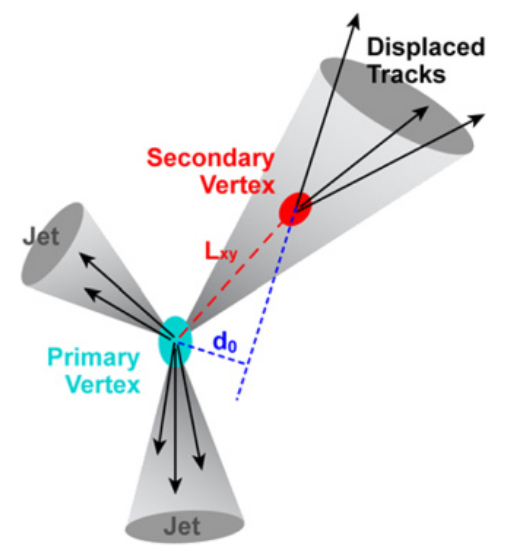
\includegraphics[width=0.5\textwidth]{Figures/CSV.png}
\end{center}
\caption{Schematic showing a displaced secondary vertex due to a b-quark decay from the primary vertex forming a b-jet. The impact parameter. $d_0$, measures the displacement with respect to the primary vertex along the z-axis, and $L_{xy}$ measures the displacement from the primary vertex in the transverse plane.}
\label{fig-CSV}
\end{figure}

B-tagged jets are particularly prominent due to their large mass, $4.18 \GeVcc$, and thus a large multiplicity of charged particles are produced during hadronisation carrying the majority of the jet energy. The most commonly used b-tagging algorithm is the Combined Secondary Vertex \cite{CSV} algorithm, which takes the following input parameters:

\begin{itemize}
	\item Track multiplicity in jet.
	\item Track multiplicity at secondary vertex.
	\item Secondary vertex category.
	\item The invariant mass of charged particles from the secondary vertex must not exceed $6.6 \GeVcc$ which would surpass the mass of the bottom quark when convoluted with its uncertainties.
	\item The ratio of the sum of the track energy at the secondary vertex to the sum of track energy of all tracks in jet.
	\item $\eta$ of the secondary vertex tracks with respect to the jet axis.
	\item The distance, $L_{xy}$, in the transverse plane between the primary and secondary vertex must be greater than $100 \mum$ and be less than $2.5 \cm$.
	\item Impact parameter significance ($L_{xy}/\sigma_{L_{xy}}$) of the first track, increasing the invariant mass above the threshold for charm production of $1.5 \GeV$.  
\end{itemize}

The algorithm begins by looking for a secondary vertex with the properties listed above. Using all particles in the jet, the algorithm uses a similar Kalman Filter \cite{VertexFitting} as for the reconstruction of primary vertices in order to reconstruct secondary vertices. If a secondary vertex is not found with this information, then a `pseudo-secondary vertex' is computed using information from the tracks that are were found to not be compatible with a primary vertex. The algorithm combines all of the information from the observables and calculates a discriminating value which is used to designate whether a jet is a `light jet' (a jet that manifests from a u,d, or s quark), a charmed jet (from a c quark), or a b-tagged jet. The CSV discriminator output can be seen in Figure \ref{fig-CSV}, showing the efficiency of correctly identifying a b-jet.

\begin{figure}
\begin{center}
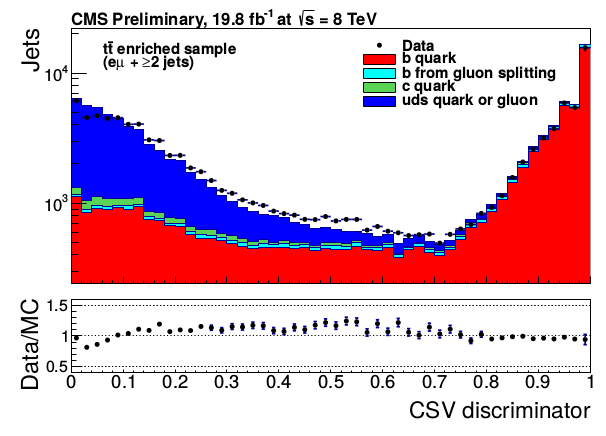
\includegraphics[width=0.8\textwidth]{Figures/CSVDiscriminator.png}
\end{center}
\caption{Logarithmic distribution of the partons as a function of the CSV b-tagging discriminant \cite{PhilThesis}.}
 \label{fig-CSVDiscriminator}
\end{figure}


\subsection{Reconstruction of Missing Transverse Energy} \label{subsec-METReco}

The conservation of momentum dictates that in an event, the sum of the $p_T$ of all final state particles (partons) must be equal to 0, as would be the case in a perfect detector. However, this is not the case within the CMS detector as particles, such as underlying events and proton remnants, are able to traverse the detector without being reconstructed. This introduces an imbalance in the measured transverse energy deposited in the detector, which we call the Missing Transverse Energy (MET). We can define the MET in an event to be:

\begin{equation}
E^{miss}_T = - \sum_i(p^2_x + p^2_y)^{1/2}
\end{equation}

where $p_x$ and $p_y$ are the transverse momenta of reconstructed particles (partons) in the x and y axes.

The reconstruction of MET is of particular importance when dealing with a measurement where the presence of weakly-interacting standard model particles are measured in the final state, such as neutrinos.  With respect to the $t\bar{t}+\gamma$ analysis, we expect a large amount of MET due to the presence of two neutrinos in the final state for each decay mode (excluding the $e\mu$ channel) of the di-lepton channel, as the W from the top quark will for decay to a lepton-neutrino pair $1/9th$ of the time. These channels, and other similar analysis, rely on the efficient reconstruction of MET in order to accurately measure certain processes, and any misidentification or poorly reconstructed particles add to the MET sum further reducing the accuracy of a measurement.  

Various methods on the reconstruction of MET in events have been conducted and are available \cite{1748-0221-6-09-P09001}. The current most accurate method for the measurement of the MET is by using the PF algorithm, and is used throughout this analysis. The PF algorithm calculates the value of the MET from the list of PF particles, thus producing a `raw' MET output which is systematically different from the final MET calculation. The `raw' MET value is calculated without taking into account the non-linearity of the calorimeters, noise from electronics, pile-up, along with any other effects. We, therefore, implement a set of corrections as described below.

\begin{description}
	\item[Type-0] corrects for the effects of pule-up on the MET.
	\item[Type-1] propagates the jet energy corrections into the MET (See Section \ref{subsec-JEC}). 
	\item[xy-shift] corrects for $\phi$ modulation in the MET.
\end{description}

The source of the $\phi$ modulation arises from misalignment of the detector relative to the beam, beam-spot displacement, an anisotropic detector response, and also broken or inactive cells within the calorimetry system. The correction for the shift in x-y is implemented in order to restore the spherical symmetry of events, and flatten the distribution in $\phi$, thus correcting the measured distribution to the true distribution. This analysis makes use of all correction types using PF calculated MET. 

\chapter{Event Selection \& Background Estimation} \label{chap-EventSelection}

When we finally arrive at a point when we have identified and reconstructed all the objects in the data, as described in Section \ref{chap-EventReconstruction&Simulation}, we impose a set of kinematic and topological cuts to each of the objects in order to provide a subset of the data containing mainly our signal events. The signal sample still contains background events and is corrected in several ways. Simulated MC samples are produced and used to optimise the number of signal events within this sample, and thus rejecting as much background as possible. The selection process, including kinematic, topological, and fiducial cuts on our final state objects is described in detail in the first part of this chapter.

Even though we model data using simulated MC samples, which are an essential tool for modelling distributions in particle physics, this is not always enough to provide a robust and accurate measurement of a process. In this case, additional methods for the calculation of background processes are used to purify our signal sample by removing events that are not in fact our final state signal event. These methods can be MC-driven and data-driven, and both are described in the second part of the chapter in greater detail pertaining to the $t\bar{t}+\gamma$ analysis.  

\section{Event Selection} \label{sec-EventSelection}

Skim
Preselection then photon selection

For the $t\bar{t}+\gamma$ analysis the selection of objects is computed in three stages; A \textbf{skim} is implemented when processing signal and background MC samples in order to reduce the rate of events at analysis level and become much more manageable, a \textbf{pre-selection} of $t\bar{t}$ events is then computed for each final state respectively following the recommended top event selection group reference, and finally the full \textbf{selection} which includes an isolated photon radiated from top quark or its decay products.   

It is important to reconstruct the number of $t\bar{t}$ events before we can include our radiated photon such that our sample is much cleaner. 
The pre-selection events have been constructed by following the CMS recommendation for cut-based selection of top-quark pair events with the requirement of at least two jets of which at least one is a b-tagged jet. Individual objects are reconstructed based on specific criteria, such as electrons, loose electrons, muons, loose muons, jets, and photons. Then an additional set of selection requirements is applied based on the relative positions of the objects ($\Delta R$ cuts). After that, the final decision is made if the event is to be considered in the further analysis. Pre-selection cuts are described in Section \ref{sec-preselection}.

\section{Pre-selection: Selection of $t\bar{t}$ Events} \label{sec-preselection}

The pre-selection steps define our $t\bar{t}$ events before the addition of a radiated photon. The selection follows the recommended selection from the TOP Reference Selections and Recommendations (Run1) \cite{TopEventSelection} designed to select di-lepton final states with two isolated oppositely charged leptons, at least 2 jets where at least one is a b-tagged jet, and two neutrinos from missing transverse energy. All objects in the selection are reconstructed using the PF algorithm as described in Section \ref{subsec-PFAlgorithm}.  


\section{Trigger and Event Cleaning} \label{sec-TriggerAndEventCleaning}

\subsection{Trigger selection}

As the $t\bar{t}+\gamma$ analysis is studied as a di-lepton final state, the requirement of at least two oppositely charged leptons (electrons or muons only) is essential. These datasets are identified by the trigger system (as described in Section \ref{sec-Trigger}) to contain two leptons. Triggers are generally divided into two categories; single object triggers fire on one or more objects of the same flavour passing certain pre-selection requirements, such as p$_T$ and $\eta$, and cross-triggers which select two objects of different flavours as predetermined by the user. For this analysis, both types of triggers are implemented in order to select the three final states in question. The list of trigger paths can be seen in Table \ref{tab-HLTriggers}. 

\begin{table} \label{tab-HLTriggers}
\begin{center}
\begin{tabular}{|c|p{11.5cm}|}
\hline
	\textbf{Final State} & \textbf{High Level Trigger Path} \\
\hline
	$\mu^+\mu^-$ & HLT\_Mu17\_Mu8\_v* \\
	$e^+e^-$ & HLT\_Ele17\_CaloIdT\_CaloIsoVL\_TrkIdVL\_TrkIsoVL
				\_Ele8\_CaloIdT\_CaloIsoVL\_TrkIdVL\_TrkIsoVL\_v* \\
	$e\mu$ & HLT\_Mu17\_Ele8\_CaloIdT\_CaloIsoVL\_TrkIdVL\_TrkIsoVL\_v*, HLT\_Mu8\_Ele17\_CaloIdT\_CaloIsoVL\_TrkIdVL\_TrkIsoVL\_v*s \\
\hline	
\end{tabular}
\caption{Triggers for each di-lepton channel.}
\end{center}
\end{table}

Each trigger path name explains the selection requirements on the objects that it triggers on. The term Mu refers to a reconstructed muon and Ele refers to a reconstructed electron, where the succeeding number represents an associated energy threshold of the particle. For example, the the di-muon channel uses a single flavour object trigger to select two muons and is used with the requirements that one of the muons has a p$_T$ greater than 8 $\GeV$ and the second greater than 17 $\GeV$. The version of the trigger is denoted in the trigger path as v*, as the trigger path changes with the trigger table used. It should be noted that a different trigger version does not in fact require a change in trigger path. At this level the number of energy deposits within the calorimetry is still too large for the trigger rate to be usable, and thus extra selection requirements on the trigger system must be imposed.

A way to reduce the trigger rate is to impose cuts on the energy threshold of the particles in question greater than that required by the trigger, however this holds drawbacks for analyses who then wish to implement tighter cuts within offline analysis. Another method, and one that is used primarily in electron trigger studies, is to reduce trigger rates to a more feasible level is to introduce isolation and Id cuts, the `Iso' and `Id' terms that can be seen in the di-electron and $e\mu$ trigger path names. The objects must then also pass simple isolation and id criteria and thus reducing the trigger rate. The information for each is obtained from both the calorimeter (e.g CaloIso) and tracker (e.g TrkId) by placing requirements on such parameters as the shape of the energy cluster, the total number of energy depositions, and the angular separation between the ECAL and tracker energy deposits. Three categories of selection are implemented for each kinematic cut, and are listed as Tight (T), Loose (L), and Very Loose (VL) as can be seen in the trigger paths. These signify the harshness of the cuts when applied. This can be visualised, for example, in the the di-electron channel where the HLT calls for two electrons, where one must pass an energy threshold of 8 $\GeV$ with a tight requirement on calorimeter Id, and very loose requirements on calorimeter isolation and tracker Id and isolation. The other electron must pass an energy threshold of 17 $\GeV$ with the same calorimeter and tracker isolation and Id cuts.

HLTs are used for the $t\bar{t}+\gamma$ analysis such that if the event does not pass the requirement of the trigger, then it is not included in the calculation. Single object triggers are used for both the di-muon and di-electron channels, and two cross-triggers were used for the $e\mu$ channel as the final state selection requires two oppositely charged leptons (electrons or muons) where one is an electron and the other a muon. The triggers were processed specifically for the $\sqrt{s}=8 \TeV$ data-taking period with 19.6 $\fbinv$.

\subsection{Filtering}

Known anomalies derived from detector and accelerator effects are a prominent feature in the processing of data. To counter these effects we incorporate several `cleaning' filters after trigger selection, but before any further selection cuts are applied. The first of which vetoes on \textbf{beam scraping} and includes a \textbf{tight CSC Beam Halo Filter}. We find that, even with the accuracy and precision that the LHC provides on accelerating bunches of protons, protons have a tendency to diverge radially from the bunch and form what is known as the beam halo that circulates the accelerator with the bunch. In early analyses it was found that the beam halo particles can be picked up in the detectors and be reconstructed as being part of an event in which it is not. Due to sensitivity to beam halo particles in the muon detectors, a filter is introduced based on muon tracking kinematics and thus veto on such events. Beam halo particles can also be removed from the beam within the LHC by introducing collimating blocks around the beam line at various points on the accelerator. This, however, presents another problem in the form of showering as the particles interact with the collimator blocks, beam scraping, and be detected by the experiments. These events are accounted for and removed from analyses by introducing the requirement that at least 25\% of reconstructed tracks within the inner detector pass the high purity threshold (see Section \ref{subsec-ChargedParticleTracking}). 

Similarly, we employ a \textbf{HCAL noise filter} in order remove events with anomalous noise within the HCAL. CMS expects a certain degree of noise, stemming from the electronic of the detector, to be present when recording data, however the majority of anomalous noise is found to originate in the Hybrid Photo-Triodes (HPT) and their corresponding read-out boxes. At the current energy scale this is not a problem as the noise appears as large, isolated energy deposits. Anomalous events have easily-identifiable signatures such as the isolation and isolation of the HCAL readout, and the multiplicity in the read-out boxes. So, if a signal demonstrates very little change in the pulse shape over time, and the read-out boxes display a high multiplicity, then an event is rejected. The next filter system comes in the form of the \textbf{HCAL laser filter}. The need for the laser filter first manifested during the 2011 data taking period when a much greater number of events were observed than was expected - $\sim5000$ htis per event. The HCAL laser filter was then designed and introduced for the 2012 data taking period.  

%%%%%%%%%%%%%%%%%%More

\section{Di-lepton Selection and Vetoes}

For the $t\bar{t}+\gamma$ analysis leptons mark our signature for our final state events. The leptons are taken from the list of PF-reconstructed objects and then required to pass additional selection cuts to refine the events further after trigger selection in Section \ref{sec-TriggerAndEventCleaning}. Along with our signal leptons, a set of `looser' PF objects are selected as veto objects, such that our signal leptons are a subset of these objects. If an event has multiple loose selection leptons then the event is removed from the list of possible signal candidates.

The number of selected leptons differs for each decay mode, and thus three separate selections must be created for the di-muon, di-electron, and mixed channels, respectively. Cuts on leptons vary depending on the channel, but are taken from the recommended values produced by the central `Top Event Selection' group \cite{TopEventSelection}. 

\subsection{Electrons}

PF electron candidates are selected for di-electron and $e\mu$ final states if they have been identified by the GSF method, as described in Section \ref{subsec-ElectronIdentification} and pass the HLT for each channel respectively. The rates are then reduced by imposing a further set of cuts taken from the recommended top reference selection cuts \cite{TOPEGM1}. The cuts are as follows:

\begin{itemize}
	\item Passes a p$_T$ threshold of > 20 \GeV.
	\item Lies within the pseudorapidity region $|\eta| < 2.5$, excluding the EB-EE transition region $1.4442 < |\eta| < 1.5660$.
	\item The transverse IP of the electron (GSF) track with respect to the first offline primary vertex must be less than 0.04 cm. 
	\item Combined relative Particle Flow (PF) $\rho$ corrected isolation in cone 0.3 less than 0.15.
	\item Trigger version of electron multivariate discriminator Trigger MVAID greater than 0.5.
	\item Conversion rejection: there should be no extra tracks pointing in the same direction.
	\item The ratio of energy deposited in the HCAL over the energy deposited in the ECAL to be less than 0.05.
\end{itemize} 

For electrons, an additional identification process is included, which uses a multivariate analysis to combine the information of several variables to produce a discrimination value between -1 and 1, such that the greater the number the more likely the event is to be an electron, (as described in Section \ref{subsec-ElectronIdentification}). Depending on whether the HLT requires an electron or not, a different version of the discriminant is used. 

One of the main criteria for lepton selection is the requirement of isolation. Generally, we define the isolation to be the sum of the p$_T$ of the reconstructed objects within a cone by which we define the radius, and then diving by the p$_T$ of the object. If we find that this produced a small number, then we say that the object is isolated. We must, however, include the effect of event PU into the calculation of isolation, and thus we introduce a correction factor. We are able to remove charged hadron tracks from the isolation sum if they do not originate from the event's primary vertex. For the case of neutral hadrons and photons which originate from PU, an effective area is defined for the electron and then an average energy is subtracted over this area. The effective area is extended into the ECAL due to the emittance of Bremsstrahlung radiation. For the case of electrons, we can define the isolation as so

\begin{equation} \label{eq-RelativeIsolation}
I_{\rho} = \frac{I_{ChargedHadron}+max\left(I_{NeutralHadron} + I_{\gamma} - \rho \cdot Eff.Area_{electron}, 0 \right)}{p_T}
\end{equation}

such that $I_{ChargedHadron}$, $I_{NeutralHadron}$, and $I_{\gamma}$ are the are the isolation cones with a fixed radius of $\Delta R = 0.3$ containing the energy deposits for each category of particle; charged hadron, neutral hadron, and photon isolation. The $\rho$ and $Eff.Area_{electron}$ parameters are the energy density of the event and the effective area for the electron which is calculated by taking the $\eta_{SC}$ and electron p$_T$. 

When a photon produced in collisions interacts with the detector material of the inner tracker it can pair-produce two electrons, thus mimicking the signature of an electron. The false signature has been calculated to represent a large source of fake electrons. The CMS EGamma working group have developed two methods in order to mitigate the fake electron signatures from the hard scattering process: measuring missing hits within the tracker system and measuring associated secondary tracks. The first technique measures the number of hits in the layers of the tracker and looks for any missing hits in the electrons associated track. If there are any missing hits, then the electron is considered as converted and discarded. The second method requires a secondary electron/positron track such that it reconstructs the pair under a certain criteria. If a second track is not found to be within 0.02 cm in the $r - \phi$ plane and the $\cot\theta$ differs by less than 0.02 then the electron is considered a conversion. 

We define a set of loose electron candidates by applying the recommended cuts as for our signal electrons but with less stringent requirements, such that our signal electrons are a subset of the loose electrons. The difference between loose and signal electrons is given by a p$_T$ cut of $> 10 \GeV$, non-triggering ID greater than zero, and several other cuts which are implemented for the identification of signal electrons are not included for loose. The \textbf{loose electrons} are defined to have the following cuts:

\begin{itemize}
	\item Transverse momentum $p_T$ greater than 10 GeV
	\item Absolute value of pseudorapidity less than 2.5
	\item Combined relative Particle Flow (PF) $\rho$ corrected isolation in cone 0.3 less than 0.15
	\item Trigger version of electron multivariate discriminator Non-Trigger MVAID greater than 0
\end{itemize}

\subsection{Muons}

For our \textbf{signal muons}, once they have passed PF selection as described in Section \ref{subsec-MuonReconstruction}, additional cuts taken from the recommended muon physics object group (POG) \cite{TOPMUO1} are imposed as follows:

\begin{itemize}
	\item Transverse momentum p$_T$ greater than 20 \GeV.
	\item Lies within the pseudorapidity region $|\eta| < 2.4$, excluding the EB-EE transition region $1.4442 < |\eta| < 1.5660$.
	\item Combined relative Particle Flow (PF) $\rho$ corrected isolation in cone 0.4 less than 0.2
	% \item At least 5 hits in the tracker (with at least one coming from the pixel detector)
	% \item At least one hit in the muon detector
	\item Identified as a particle flow muon
	\item Identified as both a tracker and global muon
\end{itemize}

The analogous relative isolation for the signal muon candidates is pileup correction and much less complicated to compute. The technique is known as $\Delta \beta$ correction and removes the neutral hadron and photon isolation from the isolation sum within a fixed cone of radius $\Delta R = 0.4$. The relative isolation can be computed as so 

\begin{equation}
I_{\Delta \beta} = \frac{I_{ChargedHadron} + max\left(I_{NeutralHadron} + I_{\gamma} - 0.5 \cdot I_{Pileup}, 0 \right)}{p_T}
\end{equation}

where the $I_{Pileup}$ parameter is the neutral hadron energy within the cone, and the factor of 0.5 is a rough estimation of the ratio of neutral hadron to charged hadron in pileup events. We categorise a muon as being isolated if the isolation sum is less than $I_{\Delta \beta} < 0.2$ within an isolation cone of $\Delta R = 0.4$. 

The production of muons from inn-flight decays is found to be much more prominent in data than is modelled in simulation. This results in a number of fake muons being recorded. In order to account for the number of fakes, the implementation of further cuts is required such that at least one hit is required in each of the pixel detector and muon detectors, and at least 6 hits recorded in the inner tracking system with two corresponding hits in the outer muon system.  

\textbf{Loose Muons} are selected from PF muons failing the muon selection that have, and are selected to have less severe requirements as listed below:

\begin{itemize}
	\item Transverse momentum $p_T$ greater than 10 GeV
	\item Absolute value of pseudorapidity less than 2.5
	\item Combined relative Particle Flow (PF) $\rho$ corrected isolation in cone 0.4 less than 0.2
	% \item At least 5 hits in the tracker (with at least one coming from the pixel detector)
	% \item At least one hit in the muon detector
	\item Identified as a particle flow muon
	\item Identified as both a tracker and global muon
\end{itemize}

\subsection{Corrections to simulated events} \label{subsec-SimulatedEventsCorrection}

\section{Jet Selection and b-tag Requirements} \label{sec-JetSelection}

Jets are reconstructed with the PF AK5 algorithm, anti-$k_T$ with jet size parameter (R) of 5 in the jet reconstruction model, and the following selections are made (PF loose Jet ID). Before applying any selection the following corrections are made to account for imperfect jet energy measurement: Jet Energy Scale correction, and Jet Energy Resolution smearing, as described in Section \ref{subsec-JetReconstruction}. After jets are identified and reconstructed, the following set of cuts are implemented with the requirements:

\begin{itemize}
	\item Transverse momentum greater than 30 GeV
	\item Absolute value of pseudorapidity less than 2.4
	\item Number of constituents greater than 1
	\item Charge multiplicity greater than 0
	\item Neutral hadron fraction of energy less than 0.99
	\item Neutral electromagnetic energy fraction less than 0.99
	\item Charged EM energy fraction less than 0.99
	\item Charged hadron energy fraction greater than 0
\end{itemize}

These cuts help to avoid picking detector noise and ECAL spikes as jets. We also impose a selection criterion that if a lepton lies within a cone of $\Delta R = 0.3$, then the lepton is included within the jet calculation. CMS improves the quality of reconstructed jets by the requirement that the energy deposits from a jet are recorded in both the ECAL and HCAL, where jets that manifest from anomalous deposits of energy in just one of the sub-detector are able to be removed from the sample \cite{CMS-PAS-JME-10-003}.

 \textbf{B-tagged jets} are identified with the Combined Secondary Vertex b-tagging algorithm using the loose working point (CSVL). Event re-weighting is applied to correct for the difference in b-tagging efficiency in data and simulation as explained in Section \ref{subsec-SimulatedEventsCorrection}. The loose working point refers to a b-tagging efficiency of  and a misidentification probability of 24.4\%.

 In each channel the requirement of at least 2 good jets, where a good jet passes all the aforementioned selection requirements, and at least one b-jet. By applying these requirements the contribution from the most prominent backgrounds, $t\bar{t}$ and events with additional loose jets, are removed. 
 

\section{Selection of $t\bar{t}+\gamma$ events} \label{sec-postselection}

From the set of $t\bar{t}$ preselected events in Section \ref{sec-Preselection}, we select only events with a photon candidate present. Main fiducial requirements are implemented as cuts in $\abs{\eta}$ and $E_T$. CMS recommended cuts are added for fiducialisation and photon selection (tight cut-based photon ID 2012 with particle flow based isolation, \cite{CutBasedIsolation2012}).In order to suppress FSR from final state particles a $\Delta R$ cut of photons between jets and leptons is applied. All simulated data is scaled to the luminosity of the recorded data used.  

\begin{description}

\item[Transverse energy] A transverse energy cut of $E_T > 25$ is implemented in order to suppress the numerous low energy fake photons and photons from other vertices other than the primary
vertex. The transverse energy distribution for each channel can be seen on the left in Figs.\ref{fig-nminusoneMuMu} --- \ref{fig-nminusoneEMu}.

\item[Pseudorapidity] An acceptance cut on the fiducial region of just the CMS ECAL barrel (EB), $\abs{\eta} < 1.4442$, is applied to verify that the electromagnetic shower of
the photon will be fully reconstructed. We will not be including the ECAL Endcap (EE) in this analysis due to the difficulty in identifying a photon thus giving very low
statistics.

\end{description}

\subsection{Cut based photon ID}

\begin{description}

\item[Electron Conversion Veto] A boolean to help distinguish an electron from a photon. We should not see a track seed in the pixel detector when identifying a photon. 

\item[Tower Based H/E] The ratio of energy deposited in the Hadronic Calorimeter (HCal) over the fraction of energy deposited in the Electromagnetic Calorimeter(ECal). This cut is
set so that the energy ratio should be less than 5\% (see Fig.\ref{fig-cutbasedMuMu1} right).

\item[Shower Width \sigma_{i\eta i\eta}] The shower shape weighted by energy (see Fig.\ref{fig-cutbasedMuMu1} right), defined as: 

\begin{equation}
\sigma_{i\eta i\eta} = \left(\frac{\sum(\eta_i - \bar{\eta})\omega_i}{\sum\omega_i}\right)^{1/2};  \bar{\eta} = \frac{\sum\eta_i\omega}{\sum\omega_i};  \omega_i = \text{max}\left(0, 4.7 +
\text{log}\frac{E_i}{E_{5x5}}\right).
\end{equation}

\item[Charged Hadron Isolation] The isolation of charged hadrons with energy density correction, $\rho$, applied. Cut given as $I_{char.had} < 1.5 GeV + 0.04*E_T(\gamma)$. See Fig.\ref{fig-cutbasedMuMu1}.

\item[Neutral Hadron Isolation] The isolation of neutral hadrons with energy density correction , $\rho$, applied. Cut given as $I_{neut.had} < 1.0 GeV + 0.005*E_T(\gamma)$. See Fig.\ref{}.

\item[Photon Isolation] The isolation of the photon $I_{\gamma}$, with energy density correction applied. Cut given as $I_{\gamma} < 1.0 GeV + 0.005*E_T(\gamma)$. See
Fig.\ref{}.

\item[super-cluster Footprint-removed Charged Hadron Isolation] The super-cluster footprint-removed isolation of charged hadrons with energy density correction, $\rho$, applied.
Cut given as $I_{char.had}(SCFR) < 5 \ \text{GeV} $. See Fig.\ref{fig-cutbasedMuMu1}.

\item[super-cluster Footprint-removed Neutral Hadron Isolation] The super-cluster footprint-removed isolation of neutral hadrons with energy density correction , $\rho$, applied.
Cut given as $I_{neut.had} < 1.0 GeV + 0.005*E_T(\gamma)$. See Fig.\ref{}.

\item[super-cluster Footprint-removed Photon Isolation] The super-cluster footprint-removed isolation of the photon $I_{\gamma}$, with energy density correction applied. Cut given
as $I_{\gamma} < 1.0 GeV + 0.005*E_T(\gamma)$. See Fig.\ref{}.

\end{description}

\subsubsection{FSR suppression}

\begin{description}
\item[\Delta R(\gamma, leptons)] In order to diminish FSR in final state leptons, e.g photons radiated off high $p_T$ muons, a minimum distance criterion in the $\eta - \phi$ plane is implemented. The cut is given as $\Delta R(\gamma, leptons) > 0.3$.

\item[\Delta R(\gamma, jets)] In order to reduce FSR in final state partons a minimum distance criterion in the $\eta - \phi$ plane is implemented. The cut is given as $\Delta R(\gamma, jets) > 0.3$.

\item[\Delta R(leptons, jets)] In order to reduce FSR in final state partons a minimum distance criterion in the $\eta - \phi$ plane is implemented. The cut is given as $\Delta R(leptons, jets) > 0.3$.
\end{description}

A significance test was performed in an attempt to optimise the $\Delta R$ cut between final state leptons and jets, however this proved inconclusive due to an initial cut of $\Delta R > 0.1$ at generator level.

\subsection{Super-cluster footprint-removal for photon isolation}

\begin{figure} \label{fig-SCFR}
\begin{center}
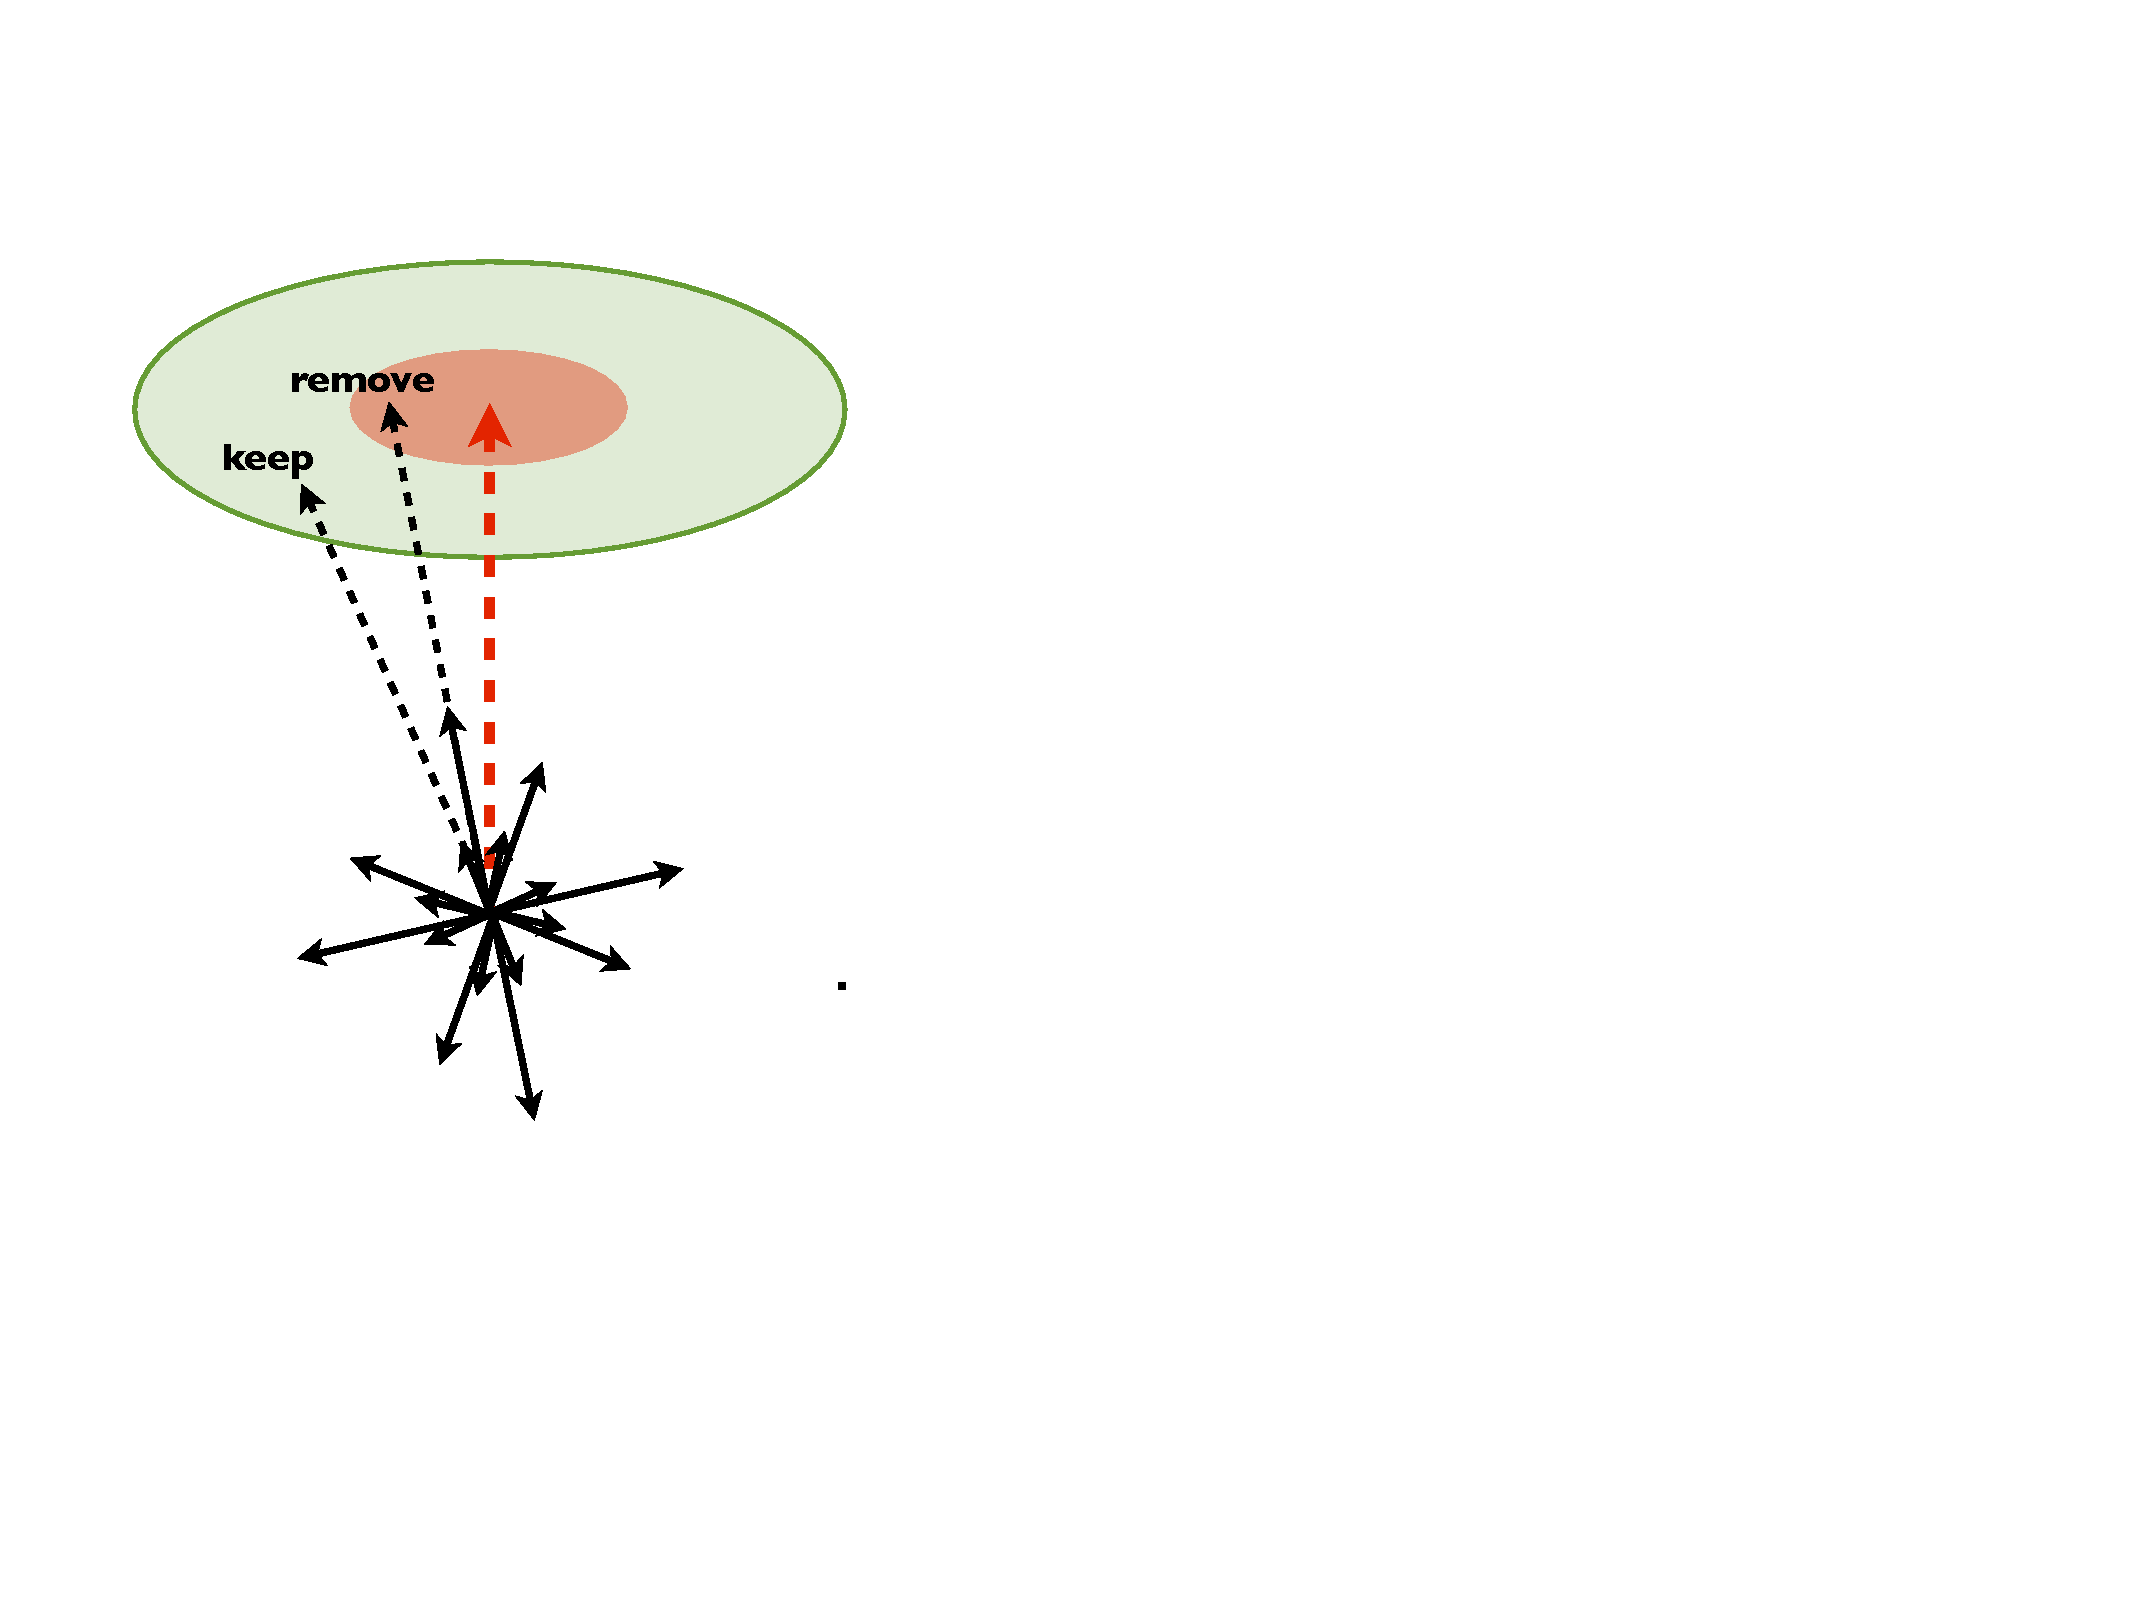
\includegraphics[width=0.4\textwidth]{Figures/RandomCone3.pdf}
\caption{}
\end{center}
\end{figure}

\section{Background Estimation}

\begin{figure} \label{fig-RandomConeIsolation}
\begin{center}
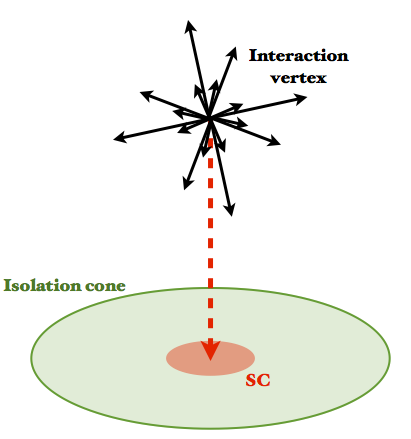
\includegraphics[width=0.45\textwidth]{Figures/RandomCone1.png}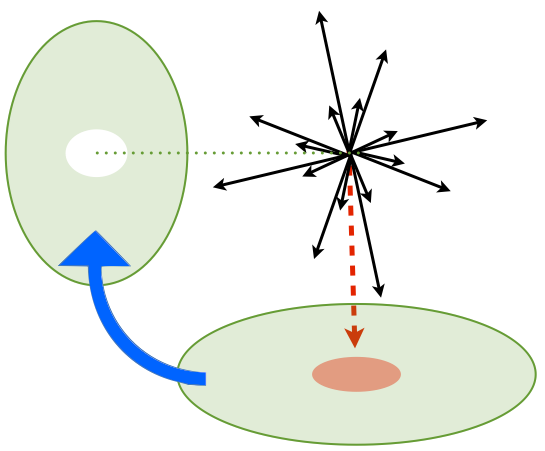
\includegraphics[width=0.55\textwidth]{Figures/RandomCone2.png}
\caption{}
\end{center}
\end{figure}

\begin{sidewaystable} \label{tab-datasets}
\begin{center}
\begin{tabular}{|l|c|c|}
\hline
	\textbf{Dataset} & \textbf{Run Range} & \textbf{Integrated Luminosity ($pb^{-1}$)}\\
\hline
	/DoubleMuParked/Run2012A-22Jan2013-v1/AOD &  & 876 \\
	/DoubleMuParked/Run2012B-22Jan2013-v1/AOD &  & 4412 \\
	/DoubleMuParked/Run2012C-22Jan2013-v1/AOD &  & 7017 \\
	/DoubleMuParked/Run2012D-22Jan2013-v1/AOD &  & 7369 \\
\hline
	Total & & 19.7\\	
\hline
	/DoubleElectron/Run2012A-22Jan2013-v1/AOD &  & 875 \\
	/DoubleElectron/Run2012B-22Jan2013-v1/AOD &  & 4412 \\
	/DoubleElectron/Run2012C-22Jan2013-v1/AOD &  & 7055 \\
	/DoubleElectron/Run2012D-22Jan2013-v1/AOD &  & 7369 \\
\hline
	Total & & 19.7\\	
\hline
	/MuEG/Run2012A-22Jan2013-v1/AOD &  & 876 \\
	/MuEG/Run2012B-22Jan2013-v1/AOD &  & 4411 \\
	/MuEG/Run2012C-22Jan2013-v1/AOD &  & 7055 \\
	/MuEG/Run2012D-22Jan2013-v1/AOD &  & 7360 \\
\hline
	Total & & 19.7\\	
\hline	
\end{tabular}	
\caption{Dataset information for each run in each respective decay channel.}
\end{center}
\end{sidewaystable}



\chapter{Measurement of the inclusive $t\bar{t}+\gamma$ cross-section}\label{chap-crosssection}

\section{Signal Definition and Background Processes}

\subsection{Signal definition}

\begin{figure} \label{fig-signalphotonplot}
\begin{center}
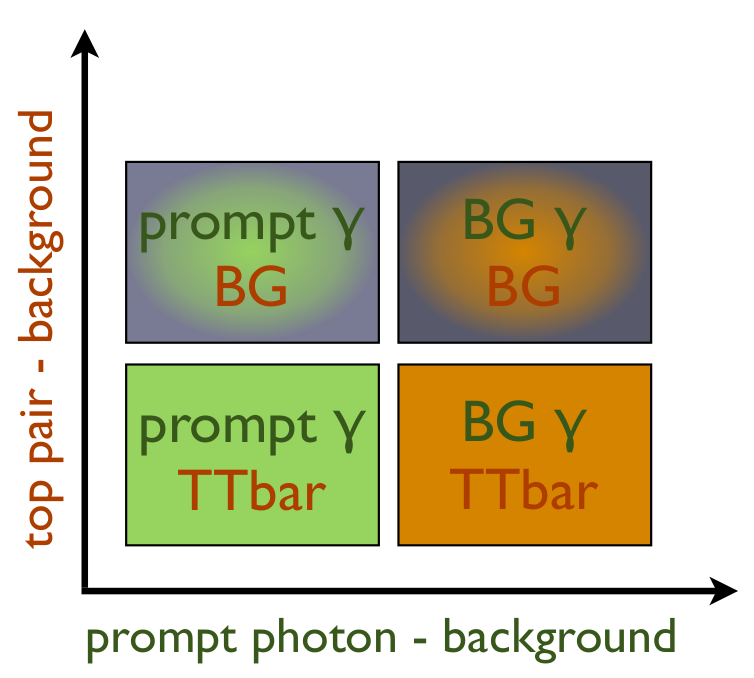
\includegraphics[scale=0.33]{Figures/SignalPhotonPlot.png}
\caption{Graphic representation of the signal and background definitions \cite{MishaSignalDefinition}.}
\end{center}
\end{figure}

\subsection{Background processes}

\begin{figure}\label{fig-AnalysisFlowChart}
\begin{center}
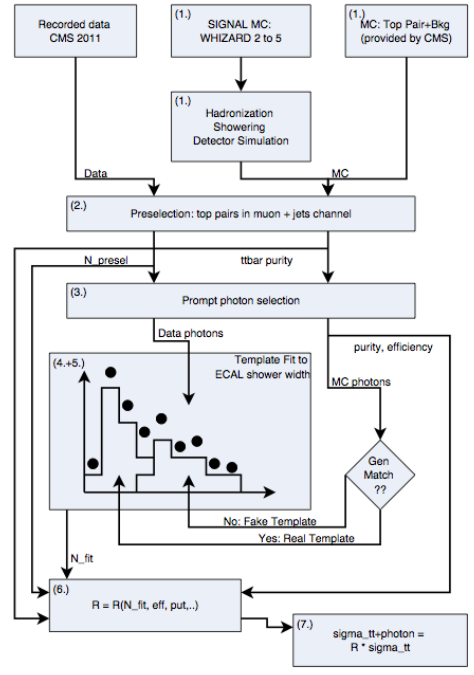
\includegraphics[width=0.75\textwidth]{Figures/AnalysisFlowChart.png}
\caption{Flow chart showing each stage of the analysis. The box numbers represent the outlined
analysis steps.}
\end{center}
\end{figure}

\section{$t\bar{t}+\gamma$ Signal Simulation}

WHIZARD

then

MADGRAPH

Factorised matrix element 

\section{Phase Space Overlap Removal} \label{sec-PhaseSpaceOverlapRemoval}

Events of the $t\bar{t}+\gamma$ process lie within a small region of $t\bar{t}$ phase space, and thus our signal sample events are expected to overlap with TTJets events in the case where a hard photon is radiated by initial state quarks, top quarks, b quarks, W and its decay products: electrons, muons, and their corresponding neutrino. In order to prevent the double counting of events we apply an overlap removal procedure to remove such events from our TTJets samples. In order for an event to be considered as overlapping with TTGamma, an event has to have at least one generator-level photon with the following properties:

\begin{itemize}
	\item p$_T(\gamma) > 13$ GeV
	\item $|\eta| < 3.0$
	\item Only gluons, bosons, or leptons are in the parents list. This ensures that photons from $\pi^0$ decays are not considered as signal
	\item $\Delta R(\gamma, other) > 0.2$ where other particles include leptons, b quarks and final state particles (hadrons, charged leptons, photons) with transverse momenta above $5 \GeV$.
\end{itemize}

The last cut is implemented in order to suppress photons from showers. In such cases the information from the parent particle will show that a photon is radiated by an electron, however the photon may be collinear with it. In particular in TTJets di-lepton events, such as described in this analysis, where a considerable fraction of the reconstructed photons comes from electrons radiating photons.

 Similarly, we also observe an overlap between Z+Jets and ZGamma processes, and between W+Jets and WGamma samples, for the same reasons as described above. The phase space overlap removal procedure is applied on Z+Jets and W+Jets samples to remove events containing generator-level photons. Events containing generated photons are removed in the case in which they are from initial state radiation (emitted from the colliding partons) or final state radiation (emitted from W or Z bosons or their decay products), since these are already included in the WGamma and ZGamma simulations. The overlap removal procedure removes approximately one percent of the events in the W+Jets sample, and approximately three to four percent of the events from the TTJets and Z+Jets samples.

\begin{figure} \label{fig-photonphasespace}
\begin{center}
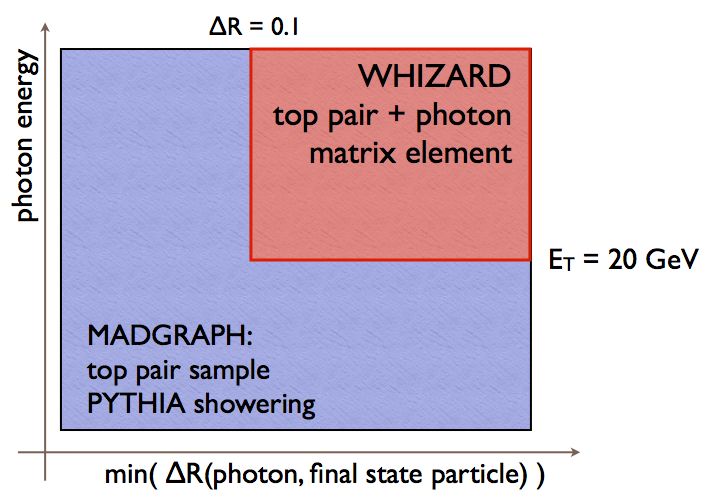
\includegraphics[scale=0.5]{Figures/photonphasespace.png}
\caption{}
\end{center}
\end{figure}

\section{Event Selection} \label{sec-EventSelection}

\section{Photon Purity Estimation} \label{sec-PhotonPurityEstimation}

\section{Signal Acceptance Calculation} \label{subsec-SignalAcceptanceCalculation}

Acceptance calculation for this analysis differs from usual inclusive cross section measurements because we measure ratio of cross sections. The event selection is chosen to make use of this fact: two steps (top selection and photon selection) are done sequentially. For the inclusive $t\bar{t}$ process, we start with number of generated events (within some fiducial phase space) and count how many events are left after top event selection. The acceptance times efficiency is defined for the $t\bar{t}$ top selection as:

\begin{equation}
	\epsilon^{t\bar{t}}_{top} \cdot A^{t\bar{t}}_{top} = \frac{N_{t\bar{t}.preselection}}{N_{t\bar{t}.generated}} 
\end{equation}

This gives the acceptance times efficiency of the inclusive $t\bar{t}$ process to be $\epsilon^{t\bar{t}}_{top} \cdot A^{t\bar{t}}_{top} =   \pm  (stat.)$ in the di-muon channel, $\epsilon^{t\bar{t}}_{top} \cdot A^{t\bar{t}}_{top} =  \pm  (stat.)$ in the di-electron channel, and $\epsilon^{t\bar{t}}_{top} \cdot A^{t\bar{t}}_{top} =  \pm  (stat.)$ in the mixed final state.

The same can be done for the $t\bar{t}+\gamma$ (signal sample). To get the acceptance times efficiency we have to divide the number of events passing top selection by the total number of events considered. However, in this case we have to choose what we take as the denominator. The signal $t\bar{t}+\gamma$ sample is inclusive, but theoretical calculations for the cross section are done for final states with 1 and 2 leptons \cite{QCDCorrectionsttgamma2011}. To make comparison with theory easier we consider the fiducial space for signal when 1 or 2 leptons are present. The $t\bar{t}+\gamma$ acceptance times efficiency of the top selection is defined for the signal samples with 1 or 2 leptons as:

\begin{equation}
	\epsilon^{t\bar{t}+\gamma}_{top} \cdot A^{t\bar{t}+\gamma}_{top} = \frac{N_{t\bar{t}+\gamma.preselection(1lor2l)}}{N_{t\bar{t}+\gamma.generated(1lor2l)}} 
\end{equation}

Giving the acceptance times efficiency of the inclusive $t\bar{t}+\gamma$ process to be $\epsilon^{t\bar{t}+\gamma}_{top} \cdot A^{t\bar{t}+\gamma}_{top} =   \pm  (stat.)$ in the di-muon channel, $\epsilon^{t\bar{t}+\gamma}_{top} \cdot A^{t\bar{t}+\gamma}_{top} =  \pm  (stat.)$ in the di-electron channel, and $\epsilon^{t\bar{t}+\gamma}_{top} \cdot A^{t\bar{t}+\gamma}_{top} =  \pm  (stat.)$ in the mixed final state.

The acceptance and efficiency for the $t\bar{t}+\gamma$ sample includes a term for photon selection. This is found based on the ratio of the number of events in $t\bar{t}+\gamma$ passing photon selection and the reconstructed photon matched to a generated photon over the number of events passing the top selection. The $t\bar{t}+\gamma$ photon selection acceptance times efficiency is defined as

\begin{equation}
	\epsilon^{t\bar{t}+\gamma}_{\gamma} \cdot A^{t\bar{t}+\gamma}_{\gamma} = \frac{N_{t\bar{t}+\gamma.photonselection(1lor2l)}}{N_{t\bar{t}+\gamma.preselection(1lor2l)}} 
\end{equation}

Thus, yields of the acceptance times efficiency of the inclusive $t\bar{t}+\gamma$ process to be $\epsilon^{t\bar{t}+\gamma}_{\gamma} \cdot A^{t\bar{t}+\gamma}_{\gamma} =   \pm  (stat.)$ in the di-muon channel, $\epsilon^{t\bar{t}+\gamma}_{\gamma} \cdot A^{t\bar{t}+\gamma}_{\gamma} =  \pm  (stat.)$ in the di-electron channel, and $\epsilon^{t\bar{t}+\gamma}_{\gamma} \cdot A^{t\bar{t}+\gamma}_{\gamma} =  \pm  (stat.)$ in the mixed final state.

The calculation of signal acceptance explained above is done for the sake of comparison with theoretical prediction. The biggest difference in the generated phase space and analysis selection is the transverse energy cut on the photon (13 GeV in generated sample and 25 GeV in analysis). We are measuring the value for the higher $E_T$ cut on the photon and using the efficiencies to extrapolate back to the full generated phase space. In order to avoid this propagation of the result into the larger phase space we also quote the \emph{visible cross section ratio}, where the cross section is measured in the fiducial region with generated photons having transverse energy of at least 25 GeV and $| \eta | < 1.4442$. For the visible cross section ratio, the photon selection term includes only the photon reconstruction efficiency because, by definition, we are considering events where generator photon passes analysis level $p_T$ and $\eta$ cuts.

The visible top selection efficiency in $t\bar{t}+\gamma$ is taken to be the ratio of the number of $t\bar{t}+\gamma$ events passing the preselection (with a generated photon having $p_T > 25$ GeV and $| \eta | < 1.4442)$

\begin{equation}
	\epsilon^{t\bar{t}+\gamma Vis}_{top} = \frac{N_{t\bar{t}+\gamma.preselection(1lor2l)}\left( p_T(\gamma_{gen}) > 25 GeV, |\eta(\gamma^{gen})| < 1.4442 \right)}{N_{t\bar{t}+\gamma.generated(1lor2l)}\left( p_T(\gamma_{gen}) > 25 GeV, |\eta(\gamma^{gen})| < 1.4442 \right)} 
\end{equation}

The $t\bar{t}+\gamma$ visible photon selection efficiency is calculated as the ratio of $t\bar{t}+\gamma$ events passing to photon selection with a reconstructed photon matched to a generated photon over the number of events passing top selection and with an isolated generator level photon passing the $p_T > 25$ GeV and $| \eta | < 1.4442$ cuts used in the photon selection.

\begin{equation}
	\epsilon^{t\bar{t}+\gamma Vis}_{\gamma} = \frac{N_{t\bar{t}+\gamma.photonselection(1lor2l)}\left( p_T(\gamma_{gen}) > 25 GeV, |\eta(\gamma^{gen})| < 1.4442 \right)}{N_{t\bar{t}+\gamma.preselection(1lor2l)}\left( p_T(\gamma_{gen}) > 25 GeV, |\eta(\gamma^{gen})| < 1.4442 \right)} 
\end{equation}

The visible top selection efficiency is found to be $\epsilon^{t\bar{t}+\gamma Vis}_{top} = 0.0712 \pm 0.0005$, $\epsilon^{t\bar{t}+\gamma Vis}_{\gamma} = 0.0928 \pm 0.0006$, and $\epsilon^{t\bar{t}+\gamma Vis}_{\gamma}$ in the di-muon, di-electron and mixed channels, respectively. The value of the visible photon selection efficiency is found to be $\epsilon^{t\bar{t}+\gamma Vis}_{\gamma} = 0.287 \pm 0.004 ( stat.)$ for the di-muon final state, $\epsilon^{t\bar{t}+\gamma Vis}_{\gamma} = 0.286 ± 0.004 (stat.)$ for the di-electron channel, and $\epsilon^{t\bar{t}+\gamma Vis}_{\gamma} = 0.287 \pm 0.004 ( stat.)$ for the mixed final state.

\chapter{Systematic Uncertainties} \label{chap-SystematicUncertainties}

Upon studying such a decay, large statistical uncertainties, comparable to the systematic uncertainties on the measurement, arise due to the small cross-section of the $t\bar{t}+\gamma$ process and small branching fraction of the decay channel. In order to perform a scientifically solid measurement we must take into account and fully understand all systematic uncertainties associated with the analysis. To begin with, we can categorise the errors into two broad categories:

\begin{description}
	\item[Flat Rate Uncertainties] - These uncertainties manifest in the form of detector performance factors, event reconstruction algorithms, and other such aspects as theoretical cross-sections which affect the overall rate of a particular process. Each uncertainty is almost universal in that it affects nearly all analyses within the collaboration, and are thus studied within their own dedicated performance group. A more detailed description can be found in \ref{sec-FlateRateUncertainties}  
	\item[Scale-factor Uncertainties] - In analyses there are often scale factors applied to scale Monte Carlo to data in order to correct for inconsistencies between the two. These can arise due to such aspects as the theoretical input parameters of the Monte Carlo generators, which are used to model signal and background processes, not taking the true shape of the data. These types of scale factors affect all distribution shapes in an analysis and therefore must be accounted, and thus an uncertainty on the scale factor is applied by varying the value up and down by one standard deviation, $\pm \sigma$, and measuring the impact that this variation has on the final result. An in-depth description of each of these types of systematic uncertainties is given in \ref{sec-ShapeUncertainties}.
\end{description}

Once computed, the systematic uncertainties are introduced as nuisance parameters within the fitting process. The final uncertainty to be considered in the fit is the statistical uncertainty that dominates this particular decay mode. This is discussed in greater detail in section \ref{chap-Results}.

% Blah blah \cite{lumiScans} \cite{PCC}

\section{Flat Rate Uncertainties} \label{sec-FlateRateUncertainties}

\subsection{Luminosity} \label{subsec-Luminosity}

The CMS collaboration measures instantaneous and integrated luminosity in two ways; one way is by means of a coincidence trigger in the forward hadron calorimeter sub-detector, and also by counting the number of clusters measured by the pixel detectors. The former method was used at the beginning of runs in the LHC, but then ran into difficulties when the number of PU increased and shifts in calibration. This lead to the development and implementation of the pixel-based calculation in 2011 - the \emph{Pixel Cluster Counting} (PCC) method \cite{cmslumiwinter2012}.

The PCC method evaluates the number of pixel clusters that occur on average for a zero-bias event (an event triggered by the requirement of only two bunches crossing at the CMS IP). It assumes that there is a small probability that each pixel within the silicon inner detector is part of more than one track per bunch crossing, and thus it is assumed that the number of pixel clusters scales linearly with the number of interactions in any given bunch crossing. This gives an excellent measure of the luminosity within the detector. Measured rates are calibrated by the method of a Van de Meer scan \cite{White:1357865}. The total calculated integrated luminosity for the entire 2012 dataset was measured to be $23.27$ fb$^{-1}$.

Although the total integrated luminosity is measured to be the value described above, the true value that we measure is less due to a number of technical reasons. Quite often a sub-detector may encounter problems at the start of the run and may require rebooting or re-calibration, thus a period of ``dead time" is induced such that data is unable to be used for physics analysis, and therefore given the title of `bad' data. The remaining measured luminosity entitled `good' is provided to analysts by the Run Coordination team, and is measured to be $19.7$ fb$^{-1}$ for the CMS experiment with the full 2012 dataset at, where a flat rate associated uncertainty of 2.6\% is assigned \cite{CMS-PAS-LUM-13-001}. Each simulated sample used in analysis is scaled to the luminosity of the dataset used, and thus the associated uncertainty affects the normalisation of every physics process.

\subsection{Lepton Efficiencies} \label{subsec-LeptonEfficiencies}

We calculate lepton efficiencies and associated uncertainties in order to correct for the number of leptons observed in data and those in simulation. In order to calculate lepton efficiencies, the tag-and-probe method is used \cite{tagandprobe}. The method analyses events from a Drell-Yan $Z \to l^+l^-$ sample as it contains a large number of unbiased lepton-pair events with a high purity. Using this sample, the tag-and-probe technique selects lepton-pair events such that one of the leptons is defined as the ``tag" lepton, which is selected with under much tighter requirements, and the second ``probe" lepton is selected under much looser constraints relative to the ``tag".  The ``tag" lepton candidate satisfies the trigger criteria, tight identification, and isolation requirements. The ``probe" lepton candidate is required to pass specific criteria depending on the efficiency under study. We thus create two subsets of the data, such that one contains events that pass the probe selection, and one collection that contains events that failed probe selection. We then take the efficiency of the selection to be the fraction of events that pass the probe selection criteria, defined as 

\begin{equation}
\epsilon_{all} = \epsilon_{reco.}\epsilon_{tight}\epsilon_{trig.}
\end{equation}

The tag-and-probe method is applied to electrons and muons separately, where it is applied to electrons in the barrel and endcap regions individually. The purity of the dilepton sample for the tag-and-probe is held by requiring the invariant mass of the lepton pair to fall within the mass window of the Z boson, $70 < M_{ll} < 130$ $\GeVcc$. We then divide the total lepton efficiency into three sub-divisions: the trigger efficiency of identifying a lepton candidate, the efficiency for the reconstruction algorithms to reconstruct leptons, and the efficiency for the identification and isolation selection requirements to correctly select leptons. 

In order to measure the trigger efficiencies for both electrons and muons, selected probes are require to pass normal kinematic cuts such that it must pass the HLT to be considered. We find that the trigger efficiency for muons is greater than 99\% and for electrons is greater than 95\%, with an associated uncertainty of the order of 4\% and varies depending on the used trigger. The reconstruction efficiency, $\epsilon_{reco.}$, is defined as the efficiency that an ECAL supercluster seeds an ECAL-driven electron candidate that passes the probe selection requirement, and is relative to ECAL clusters within the ECAL acceptance. We define the probe to have a reconstructed energy greater than 10 GeV, such that the supercluster lies within range of the tracker system. At this energy, we find the reconstruction efficiency to be greater than 85\%, and more than 99\% with an energy threshold of 20 GeV \cite{Khachatryan:2015hwa}.

For the case of muons, an initial ``preselection" of Z events for the tag-and-probe method is obtained by selecting two oppositely charged tracks measured in the central tracker that each have a $p_T > 25$ GeV, $|\eta| < 2.1$, and that when combined lie within the mass window of $60 < m_{\mu^+\mu^-} < 120$ GeV. When defining a ``tag" muon we require that it is matched to a preselected track, is a global and tracker muon, passes the selection described in Section \ref{chap-EventSelection}, and corresponds to a HLT muon. All other preselected tracks are considered as probes and are used in order to measure the efficiency. An efficiency of approximately 95-99\% is observed in data for all muon systems \cite{1748-0221-8-11-P11002}. 

The tag-and-probe method is applied to both data and simulated samples, and thus we compute the efficiency for MC simulation ($\epsilon_{sim.}$) and data ($\epsilon_{data}$).  We then compute the ratio of efficiencies along with the associated statistical and systematic uncertainties, given as:

\begin{equation}
\rho = \frac{\epsilon_{data}}{\epsilon_{sim.}}
\end{equation}

where the efficiencies and the ratios of the efficiencies are estimated in bins of E$_T$ and $\eta$ of the electron. The efficiencies and associated statistical and systematic uncertainties are derived by the EGamma and Muon Physics Object Groups (POGs) for electrons and muons, respectively.

%%%%%%%%%%%%%%%%%%%%%%%%%%%%%%%%%%%%%%%% ake sure correct and isolation/ID effs different to trig and reco.

\section{Shape Uncertainties} \label{sec-ShapeUncertainties}

\subsection{Parton Distribution Function} \label{subsec-PDFUncertainties}

Parton Distribution Functions (PDFs), denoted as $f_i(x, Q^2)$, give the probability of finding a parton of flavour $i$ (quark or gluon) carrying momentum fraction $x$ of the proton momentum where Q is the resolution scale of the hard interaction. Cross-sections are calculated by convoluting parton level cross-sections with PDFs. Due to the non-perturbative nature of partons and thus not being observed as free particles, we cannot fully obtain PDFs by perturbative QCD alone. The shapes of PDFs are determined from global fits to data from experimental observables in various processes, such as deep inelastic scattering (DIS), Drell-Yan, and jet data using the DGLAP evolution equation \cite{Vogt:2004mw}.

Event generators assign momentum fraction and energy to a parton based on PDFs which are calculated by taking data from various experiments, where each experiment has an associated uncertainty. The uncertainties must be propagated throughout the PDFs, therefore we must further propagate into our final physics analysis. PDFs are updated by the collaborations who perform the fits, such as CTEQ \cite{PhysRevD.78.013004}, each time new data or theoretical predictions become available. The set of PDFs used in this analysis are taken from the CT10 \cite{PhysRevD.89.033009} set. CT10 provides the nominal PDF weight along with 25 free parameters to describe the parton distributions, and thus 25 eigenvalues, providing 50 alternative weights per event. In order to access the weights, we use the Les Houches Accord Parton Distribution Function (LHAPDF) library \cite{Whalley:2005nh}. 

We take the difference between each of the weights and the nominal and add in quadrature, where the final result is then used to calculate the systematic uncertainty associated with the PDFs. %%%%%%%How PDF uncertainties affect the analysis



\subsection{Pile-up Re-weighting} \label{subsec-PUReweightingUncertainties}

Another example of a process that is not described well in simulation compared to data is PU. Additional pileup interactions are included within the simulated samples, however the true number of primary vertices in simulation does not match the number observed in data correctly. This discrepancy between simulation and data gives rise to an incorrect estimation of signal and/or background events in an analysis. In order to correct for this effect, additional corrections must be applied to all simulated samples. The PU re-weighting comes into fruition when dealing with the ever changing instantaneous luminosity of the beams, and thus the change in number of primary vertices in a single data-taking period. In order to implement the PU re-weighting, the number of primary vertices is re-weighted to match the current running conditions in the LHC, for example the number of primary vertices changes with the energy and luminosity of the beams. The obtained uncertainty is then included in the systematic uncertainty on the final results of the analysis. 

We take the number of primary vertices directly from the minimum bias data obtained over the running period in question. We then vary the minimum bias cross-section by $\pm5\%$ which then recalculates the primary vertex distributions which we then use to measure the total impact of the pile-up on the analysis when more, or less, pile-up is observed within the data. %%%%% PU in ttgamma

% Maybe mention out of time pileup?

\subsection{Jet Energy Corrections} \label{subsec-JECUncertainty}

As described in Section \ref{subsec-JEC}, it is necessary to apply corrections to reconstructed jet energies in order to counteract the discrepancies between generator level and detector level jets. These jet energy corrections are a set of tools included to account for non-linearities in the calorimeter, and to give a flat jet response in $\eta$ and E$_T$ as it is not trivial to translate the measured jet energy to the true particle or parton energy. The resulting jet energy corrections and associated uncertainties are measured by the JEC group who then provide the results to the collaboration to be used in analysis \cite{1748-0221-6-11-P11002, CMS-DP-2013-033}.

When we change the jet energy scale (JES) in analysis, the kinematics of each jet within an event are also modified. As a result, the number of jets that pass, or fail, the event selection requirements is likely to change, whereby altering the final topology of an event. This will have a significant impact on the final result. In order to measure the JES significance, the correction factors are varied up and down by one standard deviation, $\sigma$, and propagating the effects through to the MET. %%%Talk about results

The jet energy resolution (JER) is measured as the standard deviation of a Gaussian that is fitted to the jet response of the detector. The JER in data has been found to be worse than the JER in simulation, $\sim 10\%$ broader, and has an associated uncertainty of a similar size \cite{CMS:2011esa}. We correct for this effect by smearing the 4-momentum of jets in MC as a function of the true and reconstructed p$_T$ and $\eta$. To obtain our up and down systematic samples for the jet energy resolution, which are then included within the analysis as nuisance parameters, the smearing is applied twice for up and not at all for down. %%%Impact on JER in ttgamma

% The impact of the JER uncertainty is found to be small in
% both analyses, usually impacting event yields by less than a percent. There are notable
% exceptions to this, for example the tW Z+jets sample, but this is accounted for by the
% limited statistics in the simulated samples. 

\subsection{Missing Transverse Energy} \label{subsec-METUncertainty}

Events that contain neutrinos in the final state are affected mostly by uncertainties from modelling of MET from simulation. The way that the MET is calculated is by taking the sum of the p$_T$ of all PF-reconstructed objects, including `unclustered' energy deposits, and thus uncertainties from these propagate into the calculation of the MET. Unclustered energy is defined as recorded energy deposits that have a low p$_T$ and/or not included in a calorimeter energy deposit cluster due to isolation requirements. PF-reconstructed objects are already corrected for during the reconstruction process ($\rho$-correction, etc), however this is not the case for unclustered energy deposits. Because the unclustered energy is not corrected for during reconstruction, this is where the largest, most prominent source of uncertainty arises. In order to measure the uncertainty on the MET, we remove the p$_T$ of all PF-reconstructed objects from the MET calculation, the residual energy is scaled up and down by 10\%. Other uncertainties that affect the MET, such as JES and JER, are propagated on calculation and thus included in their respective uncertainties. Effects ee and mumu channels due to MET cut and neutrino final states %talk about effect on analysis

% effects of PU on MET distribution corrected in simulation using scale factors obtained from a Z+jets encriched control region.
% The difference between the original and scaled event yields is used as the uncertainty on the background normalisation arising from this reweighting. This uncertainty,
% which only affects the reweighted Z+jets sample in the tW search, is found to be very
% large, especially in the ttbar control regions where there are limited statistics in the simulated
% samples.



\subsection{B-tagging Efficiency} \label{subsec-BTagEfficiency}

% The b-tagging scale factors were applied differently in the
% two analyses, and the uncertainties were also, therefore, treated differently.

Studies of b-tagging efficiencies and misidentification rates are conducted by the b-tag and vertexing group (BTV) and scale factors are produced to correct for discrepancies between data and MC simulation. For the Run I data-taking period at 8 TeV, the BTV group performed studies using $t\bar{t}$ and multi-jet samples \cite{BTAGPAS}. The given samples were chosen such that studies could be performed using events with at least two jets, and a choice of the number of leptons. %b-tagging SFs in ttgamma

% \subsection{Data-driven Re-weighting} \label{subsec-DataDriverReweightingUncertainties}



% Similarly to the uncertainty introduced in Section 7.2.4, the reweighting of the recon-
% structed Z boson p T in the data driven Z+jets background estimation described in Section
% 6.2.2 also introduces a systematic uncertainty. As with the  
% E T modelling, the difference
% between the default and reweighted event yields is used as the uncertainty on the back-
% ground normalisation

\section{Modelling Uncertainties} \label{sec-ModellingUncertainties}

As well as uncertainties that affect the shape and normalisation of simulated distributions, we include uncertainty on the generator production of simulated samples. This arises due to our, possibly, limited understanding of fundamental physical principles of particle interactions in the Standard Model. It is possible that a relatively small shift in paramter value upon generation could produce significantly different events, both kinematically and topologically. We account for this uncertanty by producing alternative datasets where the values of certain parameters are increased and decreased, then by applying the standard event selection we are able to measure the shift in distribution shape from the nominal values. 

\subsection{Renormalisation and factorisation scales}

Upon generation of simulated events, we use Parton Distribution Functions (PDFs) as functions of the factorisation and normalisation scales. In simulated events they are parameterised as as one variable, known as $Q^2$. For a hard-scattering event involving a top quark, we define $Q^2$ to be $Q^2 = m^2_{top} + \sum p^2_T$. In order to calculate the uncertainty due to the renormalisation and factorisation scale, dedicated samples are produced where the $Q^2$ is ``scaled up" and ``scaled down" by a factor of 0.5 and 2.0, respectively. It is to be noted that, as the scaled samples are produced centrally, they also include variations in ISR and FSR which is central to the result in this analysis.

\subsection{Parton-level matching thresholds}

As previously mentioned, simulated events are produced using a hard-scattering generated by using the $\MADGRAPH$ matrix-element (ME) generator. However, the parton showering (PS) and hadronisation of decay products within a generated hard-scattering event is produced using the $\PYTHIA$ event generator. In order to ensure a smooth transition between the two event generators, the parton showering must be matched to the matrix element. The matching process relies on the so called k-factor MLM parton matching scale, whereby the threshold is usually set to 20 GeV \cite{Mangano:2006rw}. In order to calculate the uncertainty of the matching, dedicated samples are produced where the threshold is set to 10 and 40 Gev, respectively, which are then used to calculate the impact varying the threshold has on the final result.

We must note that this systematic only applies to samples that use matrix element to parton shower matching, and therefore does not apply to all samples used in this analysis. The samples that this applies to in this analysis are: $t\bar{t}$  %%%%

\section{Impact of uncertainties}

When a systematic uncertainty is applied, the photon purity, top quark purity, and likelihood fit are recalculated and the new value of the cross-section ratio is measured against the nominal value. Tables \ref{tab-systuncertsMuMu}, \ref{tab-systuncertsEE}, and \ref{tab-systuncertsEMu} list the calculated systematic uncertainties in decreasing order of their impact on the measured cross-section ratio for each decay channel, respectively. 

The statistical uncertainty for the number of signal events, found by maximising the likelihood fit, is the most dominant uncertainty on the cross-section calculation of the $t\bar{t}+\gamma$ process, as is expected. The measurement includes the uncertainties on the measurement of the photon purity, top purity after photon selection, and the statistical uncertainty from the number of events in data. The contribution from each process is measured individually, where the likelihood is calculated such that the uncertainty from each parameter is set to zero each time. In essence, this fixes the value to the measured value, and therefore the change in $SF_{t\bar{t}+\gamma}$ uncertainty (arounf 14\% in the standard likelihood fit) can be attributed to the fixed value. The uncertainty is dominated by the uncertainties obtained from the photon and top purity, contributing 10\% and 9\%, respectively. Therefore, the statistical uncertainty calculated from the number of events in data is approximately 4.8\%. 

\begin{table}[h!] 
\centering
\begin{tabular}{|l|c|c|}
\hline
\textbf{Source} & \multicolumn{2}{c|}{\textbf{Uncertainty (\%)}} \\ \cline{2-3}
 & Up & Down \\
\hline
Statistical & & \\
\hline
Systematic & & \\
\hline
Pileup (PU) & & \\
Out-of-time Pileup (OOT) & & \\
Top P$_{\text{T}}$ & & \\
b-tag & & \\
Photon E$_{\text{T}}$ & & \\
JEC & & \\
JER & & \\
Electron Efficiency & & \\
Electron P$_{\text{T}}$ & & \\
PDF & & \\
\hline
Total & & \\
\hline
\end{tabular} 
\caption{Systematic uncertainties and their contribution to the cross-section ratio in the $\mu^+\mu^-$ channel.}
\label{tab-systuncertsMuMu}
\end{table}

\begin{table}[h!] 
\centering
\begin{tabular}{|l|c|c|}
\hline
\textbf{Source} & \multicolumn{2}{c|}{\textbf{Uncertainty (\%)}} \\ \cline{2-3}
 & Up & Down \\
\hline
Statistical & & \\
\hline
Systematic & & \\
\hline
Pileup (PU) & & \\
Out-of-time Pileup (OOT) & & \\
Top P$_{\text{T}}$ & & \\
b-tag & & \\
Photon E$_{\text{T}}$ & & \\
JEC & & \\
JER & & \\
Electron Efficiency & & \\
Electron P$_{\text{T}}$ & & \\
PDF & & \\
\hline
Total & & \\
\hline
\end{tabular} 
\caption{Systematic uncertainties and their contribution to the cross-section ratio in the $e^+e^-$ channel.}
\label{tab-systuncertsEE}
\end{table}

\begin{table}[h!] 
\centering
\begin{tabular}{|l|c|c|}
\hline
\textbf{Source} & \multicolumn{2}{c|}{\textbf{Uncertainty (\%)}} \\ \cline{2-3}
 & Up & Down \\
\hline
Statistical & & \\
\hline
Systematic & & \\
\hline
Pileup (PU) & & \\
Out-of-time Pileup (OOT) & & \\
Top P$_{\text{T}}$ & & \\
b-tag & & \\
Photon E$_{\text{T}}$ & & \\
JEC & & \\
JER & & \\
Electron Efficiency & & \\
Electron P$_{\text{T}}$ & & \\
PDF & & \\
\hline
Total & & \\
\hline
\end{tabular} 
\caption{Systematic uncertainties and their contribution to the cross-section ratio in the $e\mu$ channel.}
\label{tab-systuncertsEMu}
\end{table}

\begin{sidewaystable}
\begin{center}
\resizebox{\textwidth}{!} {
\begin{tabular}{|l|c|c|c|} %p{11.5cm}
\hline
	Process & Dataset & $\sigma$ (pb) & Number of events \\
\hline
	$t\bar{t}$ matching up & /TTJets\_matchingup\_TuneZ2star\_8TeV-madgraph-tauola/Summer12\_DR53X-PU\_S10\_START53\_V7A-v1/AODSIM &  & 5415010 \\
	$t\bar{t}$ matching down & /TTJets\_matchingdown\_TuneZ2star\_8TeV-madgraph-tauola/Summer12\_DR53X-PU\_S10\_START53\_V7A-v1/AODSIM & & 5476728\\
	$t\bar{t}$ scale up & /TTJets\_scaleup\_TuneZ2star\_8TeV-madgraph-tauola/Summer12\_DR53X-PU\_S10\_START53\_V7A-v1/AODSIM & & 5009488\\
	$t\bar{t}$ scale down & /TTJets\_scaledown\_TuneZ2star\_8TeV-madgraph-tauola/Summer12\_DR53X-PU\_S10\_START53\_V7A-v1/AODSIM & & 5387181\\
\hline	
	Drell-Yann, $10 < m\_{ll} < 50$ &  & & \\
	Drell-Yann, $m\_{ll} > 50$ matching up & /DYJetsToLL\_M-50\_matchingup\_8TeV-madgraph-tauola/Summer12\_DR53X-PU\_S10\_START53\_V7A-v1/AODSIM & & 1985529\\
	Drell-Yann, $m\_{ll} > 50$ matching down & /DYJetsToLL\_M-50\_matchingdown\_8TeV-madgraph/Summer12\_DR53X-PU\_S10\_START53\_V7A-v1/AODSIM & & 2112387\\
	Drell-Yann, $m\_{ll} > 50$ scale up & /DYJetsToLL\_M-50\_scaleup\_8TeV-madgraph-tauola/Summer12\_DR53X-PU\_S10\_START53\_V7A-v1/AODSIM & & 2170270\\
	Drell-Yann, $m\_{ll} > 50$ scale down & /DYJetsToLL\_M-50\_scaledown\_8TeV-madgraph-tauola/Summer12\_DR53X-PU\_S10\_START53\_V7A-v1/AODSIM & & 1934901\\
\hline	
	Single Top tW scale up & /TToDilepton\_tW-channel-DR\_scaleup\_8TeV-powheg-tauola/Summer12\_DR53X-PU\_S10\_START53\_V7A-v1/AODSIM & & 1492816\\
	Single Top tW scale down & /TToDilepton\_tW-channel-DR\_scaledown\_8TeV-powheg-tauola/Summer12\_DR53X-PU\_S10\_START53\_V7A-v1/AODSIM & & 497658\\	
	Single TopBar $\bar{t}$W scale up & /TBarToDilepton\_tW-channel-DR\_scaleup\_8TeV-powheg-tauola/Summer12\_DR53X-PU\_S10\_START53\_V7A-v1/AODSIM &  & 1492534 \\
	Single TopBar $\bar{t}$W scale down & /TBarToDilepton\_tW-channel-DR\_scaledown\_8TeV-powheg-tauola/Summer12\_DR53X-PU\_S10\_START53\_V7A-v1/AODSIM &  & 1493101 \\
\hline
	W+Jets matching up & /WJetsToLNu\_matchingup\_8TeV-madgraph-tauola/Summer12\_DR53X-PU\_S10\_START53\_V7A-v1/AODSIM & & 21364637\\
	W+Jets matching down & /WJetsToLNu\_matchingdown\_8TeV-madgraph-tauola/Summer12\_DR53X-PU\_S10\_START53\_V7A-v1/AODSIM & & 21364637\\
	W+Jets scale up & /WJetsToLNu\_scaleup\_8TeV-madgraph-tauola/Summer12\_DR53X-PU\_S10\_START53\_V7A-v2/AODSIM & & 20784770\\
	W+Jets scale down & /WJetsToLNu\_scaledown\_8TeV-madgraph-tauola/Summer12\_DR53X-PU\_S10\_START53\_V7A-v1/AODSIM & & 20760884\\
\hline
\end{tabular}
}
\end{center}
\caption{Temp title}
\label{tab-systsamples}
\end{sidewaystable}

\chapter{Results} \label{chap-Results}

The values used for measuring the cross section ratio can be found in Table \ref{tab-xsectvariables}.

\begin{table}[h!]
\begin{center}
\begin{tabular}{l|c|c|c}
\hline
\hline
	\textbf{Value} & $\mu^+\mu^-$ & $e^+e^-$ & $e\mu$ \\
\hline
	Number of signal events, $N_{signal}$ & & & \\
	$t\bar{t}+\gamma$ Top Selection $\epsilon^{t\bar{t}+\gamma}_{top} \cdot A^{t\bar{t}+\gamma}_{top}$ & & & \\
	$t\bar{t}+\gamma$ Photon Selection $\epsilon^{t\bar{t}+\gamma}_{\gamma} \cdot A^{t\bar{t}+\gamma}_{\gamma}$ & & & \\
	$t\bar{t}$ Number of $t\bar{t}$ events $N^{t\bar{t}}$ & & & \\
	$t\bar{t}$ Top Selection $\epsilon^{t\bar{t}}_{top} \cdot A^{t\bar{t}}_{top}$ & & & \\
	$t\bar{t}+\gamma$ Visible Photon Selection $\epsilon^{t\bar{t}+\gamma Vis}_{\gamma} \cdot A^{t\bar{t}+\gamma Vis}_{\gamma}$ & & & \\
\hline
	Total & & & \\
\hline
\hline
\end{tabular} 
\end{center}
\caption{Values used for calculating the cross section ratios in the $\mu^+\mu^-$, $e^+e^-$, and $e\mu$ channels.}
\label{tab-xsectvariables}
\end{table}

We calculate the cross section ratios for each of the dilepton channels to be:

\begin{equation}
	R_{\mu^+\mu^-} = \frac{\sigma_{t\bar{t}+\gamma}}{\sigma_{t\bar{t}}} = \frac{N_{signal}}{\epsilon^{t\bar{t}+\gamma}_{top} A^{t\bar{t}+\gamma}_{top} \epsilon^{t\bar{t}+\gamma}_{\gamma} A^{t\bar{t}+\gamma}_{\gamma}} \cdot \frac{\epsilon^{t\bar{t}}_{top} A^{t\bar{t}}_{top}}{N_{t\bar{t}}} = 
\end{equation}

\begin{equation}
	R_{e^+e^-} = \frac{\sigma_{t\bar{t}+\gamma}}{\sigma_{t\bar{t}}} = \frac{N_{signal}}{\epsilon^{t\bar{t}+\gamma}_{top} A^{t\bar{t}+\gamma}_{top} \epsilon^{t\bar{t}+\gamma}_{\gamma} A^{t\bar{t}+\gamma}_{\gamma}} \cdot \frac{\epsilon^{t\bar{t}}_{top} A^{t\bar{t}}_{top}}{N_{t\bar{t}}} = 
\end{equation}

\begin{equation}
	R_{e\mu} = \frac{\sigma_{t\bar{t}+\gamma}}{\sigma_{t\bar{t}}} = \frac{N_{signal}}{\epsilon^{t\bar{t}+\gamma}_{top} A^{t\bar{t}+\gamma}_{top} \epsilon^{t\bar{t}+\gamma}_{\gamma} A^{t\bar{t}+\gamma}_{\gamma}} \cdot \frac{\epsilon^{t\bar{t}}_{top} A^{t\bar{t}}_{top}}{N_{t\bar{t}}} = 
\end{equation}

Another result is visible cross section ratio where we do not extrapolate the measured result to the phase space used for signal simulation. In this way we do not rely on kinematic properties of simulated signal dataset. We will need photon reconstruction and identification efficiency, but not signal acceptance for photon selection. Efficiency is calculated as ratio of number of generated signal events that passed photon selection to number of generated signal events with a generator level signal photon in the region of p$_T - \eta$ space used for photon selection (the same p$_T$ and $\eta$ cuts are applied to generated photons as used for the reconstructed photon). The visible cross section ratio is measured in each respective dilepton channel to be:

\begin{equation}
	R^{Vis.}_{\mu^+\mu^-} = \frac{\sigma_{t\bar{t}+\gamma}}{\sigma_{t\bar{t}}} = \frac{N_{signal}}{\epsilon^{t\bar{t}+\gamma Vis.}_{top} A^{t\bar{t}+\gamma Vis.}_{top} \epsilon^{t\bar{t}+\gamma Vis.}_{\gamma} A^{t\bar{t}+\gamma Vis}_{\gamma}} \cdot \frac{\epsilon^{t\bar{t}}_{top} A^{t\bar{t}}_{top}}{N_{t\bar{t}}} = 
\end{equation}

\begin{equation}
	R^{Vis.}_{e^+e^-} = \frac{\sigma_{t\bar{t}+\gamma}}{\sigma_{t\bar{t}}} = \frac{N_{signal}}{\epsilon^{t\bar{t}+\gamma Vis.}_{top} A^{t\bar{t}+\gamma Vis.}_{top} \epsilon^{t\bar{t}+\gamma Vis.}_{\gamma} A^{t\bar{t}+\gamma Vis}_{\gamma}} \cdot \frac{\epsilon^{t\bar{t}}_{top} A^{t\bar{t}}_{top}}{N_{t\bar{t}}} = 
\end{equation}

\begin{equation}
	R^{Vis.}_{e\mu} = \frac{\sigma_{t\bar{t}+\gamma}}{\sigma_{t\bar{t}}} = \frac{N_{signal}}{\epsilon^{t\bar{t}+\gamma Vis.}_{top} A^{t\bar{t}+\gamma Vis.}_{top} \epsilon^{t\bar{t}+\gamma Vis.}_{\gamma} A^{t\bar{t}+\gamma Vis}_{\gamma}} \cdot \frac{\epsilon^{t\bar{t}}_{top} A^{t\bar{t}}_{top}}{N_{t\bar{t}}} = 
\end{equation}

\begin{table}
\centering
\begin{tabular}{|l|l|}
\hline
	\textbf{Parameter} & \textbf{Value} \\
\hline
	$t\bar{t}+\gamma events$ & \\
	$t\bar{t}+\gamma eff.$ & \\
	$t\bar{t} events$ & \\
	$t\bar{t} eff$ & \\
\hline
\end{tabular}
\caption{}
\end{table}	

\chapter{Measurement of the anomalous couplings of the photon to the top quark}\label{chap-anomolouscouplings}

\chapter{Electron Conversion Veto}\label{chap-conversionveto}


\chapter*{Conclusions}\label{chap-conclusions}

In this thesis we present the observation and cross-section measurement of top quark pairs in association with a radiated photon decaying to a dilepton final state. The measurement was made using data from proton-proton collisions recorded by the CMS detector at the Large Hadron Collider, running with a centre-of-mass energy of $\sqrt{s} = 8$ TeV over the 2012 data-taking period. 

A cut-based analysis measuring the production cross-section of top quark pair events in association of a radiated photon, as well as the ratio of the production cross-section to the inclusive top quark pair cross-section, was carried out using the full 2012 dataset corresponding to an integrated luminosity of $19.7$ fb$^{-1}$. We take the ratio of cross-sections in order to cancel out global variables, such as luminosity. The estimation of the photon identification efficiency is calculated by studying the photon isolation profile using the supercluster footprint removal technique and random cone isolation. This method allows us to extract signal and background templates directly from data. The technique is cross-checked with simulated events for completeness. 

The main sources of uncertainty for the measurement manifest in the form of the purity of top pair events passing selection, and the number of photon events passing full selection. The precision of the cross-section calculation is limited due to the very small number of events passing selection. A cross-section of $\sigma_{t\bar{t}+\gamma} = 983 \pm 32$ fb and ratio $R = \sigma_{t\bar{t}+\gamma}/\sigma_{t\bar{t}} = 0.00221 \pm 0.00023$ was measured in comparison to the theoretical prediction of $\sigma_{t\bar{t}+\gamma}^{theoretical} = 861 \pm 182$ fb, using the latest measurement of the inclusive $t\bar{t}$ cross-section. Therefore, we observe a good agreement with the Standard Model and do not observe any evidence for physics beyond that of the Standard Model. This is the most accurate measurement of the $t\bar{t}+\gamma$ process to date and the only measurement in the dilepton final state ever performed.  


\section{Future Outlook}

Overall, the outlook for a measurement of the $t\bar{t}+\gamma$ process at higher energies is an exciting prospect. It will be possible to measure the cross-section of the process to a much higher degree of accuracy due to the increase in the production of top quark pairs compared to a much lower production rate of background processes. For an LHC running at centre-of-mass energy of $\sqrt{s} = 14$ TeV, we expect a cross-section for top quark pairs to have increased by $\sim3.5$ times the cross-section at $\sqrt{s} = 8$ TeV at $920$ pb \cite{Czakon:2013goa}, compared to an increase of $\sim1.5$ times that at $\sqrt{s} = 8$ TeV for background processes. This can be seen in Figure \ref{fig-ttbarXsectPlot}. This increase in top quark pair production would remove the main inhibitor of the measurement -- it is statistically limited.

Ultimately, we would like to measure the electromagnetic vertex of the top quark and radiated photon, however it could also be used in conjunction with other measurements. For example, a future $t\bar{t}+\gamma$ measurement could also be used in a way that is complementary to the search for top quark pair plus a radiated Higgs boson, whereby the Higgs decays to two photons in the final state. Understanding this process will be of huge importance as it will be a background to the $t\bar{t}+\gamma$ process, and a combination of semileptonic and dileptonic channels would be more beneficial at higher energies due to increased statistics. Similarly, understanding the $t\bar{t}+\gamma$ process is greatly import as it is a background to many SUSY processes. At higher energies it will be possible to glean a greater understanding of the process by measuring the differential cross-section with respect to global variables. 

\addcontentsline{toc}{chapter}{Conclusions}

\appendix
\appendixpage
\addappheadtotoc

\renewcommand{\thesection}{A.\arabic{section}}
\renewcommand\thefigure{\thesection}
\renewcommand\thetable{\thesection}

\section{Operator contributions to $\gamma t \bar{t}$}

Here we show the contributions to the effective $\gamma t \bar{t}$ vertices of the operators in Equation \ref{}. We use the shorthand $\alpha_x = C_x/\Lambda^2$ and drop the indices from the $\alpha$ constants.

\begin{align}
\alpha O^{33}_{uW} + \alpha^* (O^{33}_{uW})^{\dagger} & \supset \frac{v}{\sqrt{2}}s_W \lbrack \text{Re} \alpha\bar{t}\lambda^a g^{\mu \nu} t + i \text{Im} \alpha \bar{t}\lambda^a g^{\mu \nu} \gamma^5 t\rbrack G^a_{\nu} Z_{\mu}\\ 
\alpha O^{33}_{uB\phi} + \alpha^* (O^{33}_{uB\phi})^{\dagger} & \supset \frac{v}{\sqrt{2}}c_W \lbrack \text{Re} \alpha\bar{t}\lambda^a g^{\mu \nu} t + i \text{Im} \alpha \bar{t}\lambda^a g^{\mu \nu} \gamma^5 t\rbrack G^a_{\nu} Z_{\mu}\\ 
\alpha O^{33}_{qW} + \alpha^* (O^{33}_{qW})^{\dagger} & \supset s_W \lbrack \text{Re} \alpha\partial^{\nu}(\bar{t}_L\gamma^{\mu}t_L) + i \text{Im} \alpha \bar{t}_L\gamma^{\mu}\partial^{\nu}t_L \rbrack A_{\mu \nu}\\ 
\alpha O^{33}_{qB} + \alpha^* (O^{33}_{qB})^{\dagger} & \supset c_W \lbrack \text{Re} \alpha\partial^{\nu}(\bar{t}_L\gamma^{\mu}t_L) + i \text{Im} \alpha \bar{t}_L\gamma^{\mu}\partial^{\nu}t_L \rbrack A_{\mu \nu}\\ 
\alpha O^{33}_{uB} + \alpha^* (O^{33}_{uB})^{\dagger} & \supset c_W \lbrack \text{Re} \alpha\partial^{\nu}(\bar{t}_L\gamma^{\mu}t_L) + i \text{Im} \alpha \bar{t}_R\gamma^{\mu}\partial^{\nu}t_R \rbrack A_{\mu \nu}  
\end{align}

\section{Electron \& Muon Efficiencies}

\begin{table} \label{tab-ElectronEfficiencies}
\begin{center}
\resizebox{\columnwidth}{!} {
\begin{tabular}{|c|c|c|c|c|}
\hline
	\textbf{All ID and Isolation (MVA $>$ 0.5)} & $20 < p_T < 30$ & $30 < p_T < 40$ & $40 < p_T < 50$ & $50 < p_T$ \\
\hline	
	$|\eta| < 0.8$ & 0.969 $\pm$ 0.007 & 0.926 $\pm$ 0.003 & 0.969 $\pm$ 0.002 & 0.975 $\pm$ 0.000 \\
	$0.8 < |\eta| < 1.4442$ & 0.935 $\pm$ 0.017 & 0.945 $\pm$ 0.004 & 0.964 $\pm$ 0.002 & 0.974 $\pm$ 0.002 \\
	$1.4442 < |\eta| < 1.5660$ & 1.032 $\pm$ 0.039 & 0.907 $\pm$ 0.015 & 0.957 $\pm$ 0.022 & 0.877 $\pm$ 0.020 \\
	$1.5660 < |\eta| < 2.5$ & 0.919 $\pm$ 0.014 & 0.926 $\pm$ 0.005 & 0.952 $\pm$ 0.003 & 0.950 $\pm$ 0.005 \\
\hline	
\end{tabular}
}
\caption{Electron ID \& isolation efficiencies \cite{ElectronEfficiencies}.}
\end{center}
\end{table}

\begin{table} \label{tab-MuonEfficiencies}
\begin{center}
\begin{tabular}{|c|c|}
\hline
	\textbf{All ID and Isolation} & $p_T > 20$ GeV/c \\
\hline	
	$0 < |\eta| < 0.9$ & 0.9984 $\pm$ 0.0002 \\
	$0.9 < |\eta| < 1.2$ & 0.9990 $\pm$ 0.0002 \\
	$1.2 < |\eta| < 2.1$ & 0.9986 $\pm$ 0.0001 \\
	$2.1 < |\eta| < 2.5$ & 1.0000 $\pm$ 0.0003 \\
\hline	
\end{tabular}
\caption{Muon ID \& isolation efficiencies \cite{MuonEfficiencies}.}
\end{center}
\end{table}

\bibliography{PhDThesis}
\bibliographystyle{unsrt}
\addcontentsline{toc}{chapter}{Bibliography}
\end{document}
